\documentclass[11pt]{article}
\RequirePackage{fullpage}
\RequirePackage[font=small,labelfont=bf]{caption}
\RequirePackage{amsmath,amssymb,amsthm}
\RequirePackage{mathtools}
\RequirePackage{graphicx}
\RequirePackage[normalem]{ulem}
\RequirePackage[hidelinks]{hyperref}
\RequirePackage{subcaption}
\RequirePackage{wasysym}
\RequirePackage{authblk}
\RequirePackage{bm}
\RequirePackage{bbm}
\RequirePackage{tikz}

% line numbers:
\RequirePackage{lineno}
%\modulolinenumbers[5]
%\definecolor{linenogray}{black}{0.75}
%\renewcommand\linenumberfont{\normalfont\tiny\sffamily\color{linenogray}}

% spacing
\RequirePackage{setspace}
%\doublespacing
 
% \RequirePackage[osf]{mathpazo}
\RequirePackage[bibstyle=authoryear,citestyle=authoryear-comp,
                date=year,
                maxbibnames=9,maxnames=5,maxcitenames=2,
                backend=biber,uniquelist=false,uniquename=false,
                % style=apa,
                % sorting=nyt,
                sorting=ynt,
                hyperref=true]{biblatex}
\RequirePackage[colorinlistoftodos]{todonotes}  %disable
\RequirePackage{color}
\RequirePackage{nicefrac}

\newcommand{\gc}[1]{{\it \color{red} #1 } }
\newcommand{\vb}[1]{{\it \color{blue} #1}}
\newcommand{\vbout}[1]{{\it \color{blue} \sout{#1}}}

% a /nonumber you can turn on/off
\newcommand{\nnn}{\nonumber}
%\newcommand{\nnn}{}


\newcommand{\graham}[1]{\todo[size=\scriptsize, color=red!50]{#1}}
\newcommand{\vince}[1]{\todo[size=\scriptsize, color=blue!50]{#1}}

\renewcommand{\P}{\mathbb{P}}
\newcommand{\E}{\mathbb{E}}
\newcommand{\V}{\text{V}}
\newcommand{\cf}{\emph{cf.} }
\DeclareMathOperator{\var}{Var}
\DeclareMathOperator{\cov}{Cov}
\DeclareMathOperator{\T}{{\mathrm{T}}}
\newcommand{\vect}[1]{\mathbf{#1}}
\newcommand{\nssh}{SSH_n}

\newcommand{\chapquote}[2]{\begin{quotation} \textit{#1} \end{quotation} \begin{flushright} - #2\end{flushright} }

\addbibresource{temporal-covariance.bib}

% \title{Linked Selection During Rapid Polygenic Adaptation Creates an Autocovariance Signal Detectable from Temporal Data}
% \title{A temporal signal of polygenic linked selection}
%\title{A Linked Selection Signal During Rapid Polygenic Adaptation from Temporal Data}
% \title{Rapid Polygenic Adaptation Creates a Detectable Signal of Linked Selection in Temporal Data}
\title{The Linked Selection Signature of Rapid Adaptation in Temporal Genomic Data}

\author[$\ast$,$\dag$,$1$]{Vince Buffalo}
\author[$\dag$]{Graham Coop}
\affil[$\ast$]{\footnotesize Population Biology Graduate Group}
\affil[$\dag$]{\footnotesize Center for Population Biology, Department of Evolution and Ecology, University of California, Davis, CA 95616}
\affil[$1$]{\footnotesize Email for correspondence: \href{mailto:vsbuffalo@ucdavis.edu}{vsbuffalo@ucdavis.edu}}

\begin{document}
\maketitle


\linenumbers
\begin{abstract}

  The majority of empirical population genetic studies have tried to understand
  the evolutionary processes that have shaped genetic variation in a single
  sample taken from a present-day population.  However, genomic data collected
  over tens of generations in both natural and lab populations are increasingly
  used to find selected loci underpinning adaptation over these short
  timescales. Although these studies have been quite successful in detecting
  selection on large-effect loci, the fitness differences between individuals
  are often polygenic, such that selection leads to allele frequency changes
  that are difficult to distinguish from genetic drift. However, one promising
  signal comes from polygenic selection's effect on neutral sites that become
  stochastically associated with the genetic backgrounds that lead to fitness
  differences between individuals.  Previous theoretical work has established
  that the random associations between a neutral allele and heritable fitness
  backgrounds acts to reduce the effective population size experienced by this
  neutral allele \parencite{Santiago1995-hx,Santiago1998-bs}. These
  associations perturb neutral allele frequency trajectories, creating
  autocovariance in the allele frequency changes across generations. Here, we
  show how temporal genomic data allows us to measure the temporal
  autocovariance in allele frequency changes and characterize the genome-wide
  impact of polygenic selection. We develop expressions for these temporal
  autocovariances, showing their magnitude is determined by the level of
  additive genetic variation, recombination, and linkage disequilibria in a
  region. Furthermore, by using analytic expressions for the temporal variances
  and autocovariances in allele frequency, we demonstrate that one can estimate
  the additive genetic variation for fitness and the drift-effective population
  size from temporal genomic data. We also show how the proportion of total
  variation in allele frequency change due to linked selection can be estimated
  from temporal data. Overall, we demonstrate temporal genomic data offers
  opportunities to identify the role of linked selection on genome-wide
  diversity over short timescales, and can help bridge population genetic and
  quantitative genetic studies of adaptation.

 \end{abstract}

Adaptation can occur over remarkably short ecological timescales, with
dramatic changes in phenotype occurring over just a few generations in natural
populations. This rapid pace of adaptive change has been known to be mirrored
at the genetic level since the early work of \textcite{Fisher1947-tf}  testing
whether the rapid decline in a coloration polymorphism was consistent with
natural selection or genetic drift. Since then, researchers have continued to
use temporal data to detect selection on polymorphisms over short timescales in
natural populations
\parencite{Kettlewell1958-or,Kettlewell1961-ok,Fisher1947-tf,Dobzhansky1943-lh,Dobzhansky1971-vf,Mueller1985-eo},
as well as quantify the rate of genetic drift
\parencite{Nei1981-oy,Pollak1983-xh,Mueller1985-eg,Waples1989-sj,Wang2003-ev,Prout1954-yy,Wallace1956-jb}.
However, this line of work in sexual populations has been partially eclipsed by
a vast body of work examining large-scale population-genetic and -genomic data
sets from a single contemporary timepoint. More recently, studies have applied
similar temporal approaches to whole-genome data to discover selected loci in
contemporaneous natural populations
\parencite{Bergland2014-ij,Rajpurohit2018-od}, evolve and re-sequence studies
\parencite{Burke2010-tz,Johansson2010-ya,Teotonio2009-sa,Turner2011-sx,Turner2012-bm,Franssen2017-lx,Orozco-terWengel2012-fu,Barghi2019-qy},
and ancient DNA \parencite{Mathieson2015-uw,Fu2016-ek}. Furthermore,
  numerous methods have been developed to estimate effective population size
\parencite{Pollak1983-xh,Waples1989-sj,Nei1981-oy} and detect selected loci
\parencite{Feder2014-lc,Mathieson2013-we,Terhorst2015-rg,Malaspinas2012-aw}
from time-series data.

Overall, these approaches have identified compelling examples where selection has driven
extreme allele frequency change at particular loci that is inconsistent with
drift alone.  However, most adaptation on ecological timescales likely involves
selection on phenotypes with polygenic architecture and abundant standing
variation \parencite{Endler1986-wd,Hendry1999-zu,Kinnison2001-vb,Kopp2009-pj}.
We know from theory that adaptation on such traits can result from very subtle
allele frequency changes across the many loci that underlie the trait
\parencite{Bulmer1980-zo}, at least for the short-term evolutionary response
\parencite{Jain2017-mw,Jain2015-xy,Thornton2018-eo,Chevin2008-lt,Hermisson2005-hs,Hollinger2019-mn}.
These changes may be individually indistinguishable from genetic drift in
temporal data. This poses a challenge for population genetic approaches to
quantify selection: rapid phenotypic adaptations occurring on ecological
timescales may leave a signal on genome-wide patterns of diversity that is
undetectable by methods focused on individual loci.

Here, we explore an alternative: rather than aiming to find selected loci, we
can use temporal data to quantify the genome-wide effects of linked selection
during polygenic adaptation. Linked selection introduces a new source of
stochasticity into evolution, as a neutral allele's frequency change depends on
the fitness of the set of random genetic backgrounds it finds itself on
\parencite{Gillespie2000-mh}. The impact linked selection has on neutral loci
is mediated by associations (linkage disequilibria, or LD) with selected loci
and hence their recombination environment; neutral loci tightly linked to
selected sites experience greater average reductions in diversity than more
loosely coupled sites. Studies using a single timepoint have long exploited
this idea, with some of the first evidence of pervasive natural selection being
the correlation between diversity and recombination in \emph{Drosophila}
\parencite{Aguade1989-jx,Begun1992-ey}. Various forms of linked selection give
rise to such patterns with much attention focusing on the hitchhiking (positive
selection; \cite{Maynard_Smith1974-lc}), or background selection models
(negative, or purifying selection; \cite{Charlesworth1993-gb,Hudson1995-xc}).
Recent genomic studies have modeled patterns of genome-wide diversity
considering substitutions, functional constraint, and recombination
environments to estimate parameters of hitchhiking and background selection
models, and have begun to differentiate between these models
\parencite{McVicker2009-ax,Hernandez2011-gs,Elyashiv2016-vt}.  Across-taxa
comparisons have shown that signals of linked selection are present in many
sexual organisms, and that in some species a proportion of the stochastic
change in allele frequencies is due to the randomness of linked selection
instead of genetic drift
\parencite{Cutter2013-ba,Corbett-Detig2015-gt,Coop2016-gx}. Likewise, in
asexual and facultatively sexual organisms both theory and empirical work show
that linked selection and interference are a primary determinant of the levels
of genetic diversity
\parencite{Neher2011-fy,Neher2013-dz,Good2017-om,Good2014-yz}.

In this paper, we extend this well-established approach of quantifying
genome-wide selection through its indirect impact on linked neutral sites to
temporal genomic data. We show that during rapid polygenic selection, linked
selection leaves a signal in temporal genomic data that can readily be
differentiated from neutral processes. Specifically, selected alleles perturb
the allele frequency trajectories of neighboring neutral loci, increasing the
variance of neutral allele frequency change and creating covariance between the
neutral allele frequency changes across generations.  Earlier work has modeled
this effect on neutral alleles as a long-term reduction in the effective
population size
\parencite{Robertson1961-ho,Santiago1995-hx,Santiago1998-bs,Wray1990-zf,J_A_Woolliams_N_R_Wray_R_Thompson2008-qo},
but the increasing availability of genome-wide frequency data across multiple
timepoints allows us to directly quantify the extent of linked selection over
short ecological timescales (tens of generations). We develop theory for the
variances and covariances of neutral allele frequency change under selection,
and show that analogous to diversity in a single timepoint study, their
magnitude depends on the local fitness variation, recombination, and linkage
disequilibria. Furthermore, we show that our theory can (1) directly
partition the variation in genome-wide frequency change into the components
caused by drift and selection, (2) estimate the additive genetic
variance for fitness and how it changes over time, and (3) detect patterns of
fluctuating selection from temporal data. Overall, we believe our approach to
modeling temporal genomic data will provide a more complete picture of how
selection shapes allele frequency changes over ecological timescales in natural
populations, potentially allowing us to understand short-term effects of linked
selection that would otherwise not be perceptible from studies using a single
timepoint. 

\section{Outline of Temporal Autocovariance Theory}
\label{sec:outline-temp}

Our goal is to understand how linked selection affects the frequency
trajectories of neutral sites by modeling the variances and covariances of
neutral allele frequency changes ($\Delta p_t = p_{t+1} - p_t$, where $p_t$ is
the population frequency at time $t$). We assume a closed population with
discrete, non-overlapping generations. When there are no heritable fitness
differences between individuals, genetic drift is the only source of
stochasticity of allele frequency change due to two sources of variation:
random non-heritable, or environmental differences in offspring number, and
Mendelian segregation of heterozygotes. Both are directionless such that when
averaged over evolutionary replicates, the expected change in allele frequency
due to drift alone is $\E(\Delta p_t) = 0$ and quantified by the variance in
allele frequency change $\var(\Delta p_t)$ \parencite[as quantified by the
variance effective population
size;][]{Wright1938-tv,Crow1970-wm,Charlesworth2009-sg}.

% We first give an outline of how selection affects linked neutral sites through
% time. We summarize a neutral allele's frequency trajectory as the differences
% in adjacent timepoints, $\Delta p_t = p_{t+1} - p_t$, where $p_t$ is the
% population frequency at time $t$, and we assume a closed population with
% discrete, non-overlapping generations. While throughout the paper we assume
% that allele frequencies can be measured every generation, the same approach can
% be extended to situations where the study system cannot be observed every
% generation. Our goal is to understand how linked selection affects the
% frequency trajectories of neutral sites by modeling the variances and
% covariances of neutral allele frequency changes. Before considering the impact
% of linked selection, we first consider a population that lacks heritable
% fitness differences between individuals. In this case, the stochasticity of
% allele frequency change is determined entirely by two components: random
% non-heritable, or environmental differences in offspring number, and Mendelian
% segregation of heterozygotes. These two sources of stochasticity are
% collectively known as drift, and both are directionless such that when averaged
% over evolutionary replicates, the expected change in allele frequency due to
% drift alone is $\E(\Delta p_t) = 0$. The magnitude of drift's stochastic
% effects are quantified by the variance in allele frequency change $\var(\Delta
% p_t)$, which in a Wright--Fisher model of reproduction where offspring number
% has a multinomial distribution, is $\var(\Delta p_t) =
% \nicefrac{p_t(1-p_t)}{(2N)}$. Different mating systems and higher non-heritable
% variance in offspring number can be accommodated under the Wright--Fisher model
% by replacing $N$ with $N_e$, the variance effective population size
% \parencite{Wright1938-tv,Crow1970-wm,Charlesworth2009-sg}.

When there are heritable fitness differences between individuals in the
population, a third source of stochasticity affects a neutral allele's
frequency change: neutral alleles can become randomly associated with the
genetic backgrounds that determine the fitness differences between individuals
\parencite{Robertson1961-ho,Santiago1995-hx,Santiago1998-bs}. Even though the
neutral alleles do not impact fitness, their frequency trajectories are
perturbed by their fitness background, as those on advantage backgrounds leave
more descendants, while those on disadvantageous backgrounds leave fewer. We
can partition a neutral allele frequency's change into these three uncorrelated
stochastic components (following \citeauthor{Santiago1995-hx},
\citeyear{Santiago1995-hx}, see our Appendix Section \ref{ap:decomp} for
proof),

\begin{align}
  \Delta p_t %&= p_{t} - p_{t-1}  \\
  &= \underbrace{\Delta_{_N} p_t + \Delta_{_M} p_t}_\text{drift} + \underbrace{\Delta_{_H} p_t}_\text{selection}
  \label{eq:delp-decomp}
\end{align}
%
where, $\Delta_{_N} p_t$, $\Delta_{_M} p_t$, and $\Delta_{_H} p_t$ are the
neutral allele's frequency changes due to non-heritable variation in fitness
between diploid individuals, Mendelian segregation of heterozygotes into
offspring, and heritable variation in fitness (we refer to this as the
\emph{heritable change} in neutral allele frequency), respectively. Note that 
  while throughout the paper we consider the allele frequency change between
  adjacent generations, the same approach can be extended to situations where
the study system cannot be observed every generation. Like the stochastic
components of drift, the allele frequency change due to heritable fitness
differences is directionless ($\E(\Delta_{_H} p_t) = 0$).
Additionally, since each component is uncorrelated with the others, the
variance in allele frequency change is

\begin{align}
  \var(\Delta p_t) &= \var(\Delta_{_N} p_t)  + \var(\Delta_{_M} p_t) + \var(\Delta_{_H} p_t).
  \label{eq:var-decomp-1}
\end{align}
%
The terms $\var(\Delta_{_N} p_t)$ and $\var(\Delta_{_M} p_t)$ capture the
variance due to the random reproduction process, and the former can accommodate
extra non-heritable variance in offspring number (as long as individuals are
exchangeable with respect to their genotype; \cite{Cannings1974-ps}), while the
term $\var(\Delta_{_H} p_t)$ captures heritable fitness variation due to
systematic differences in the fitness of individuals caused by their genotypes.

In addition to inflating the within-generation variance in allele frequency
change, heritable fitness variation has another profound affect on neutral
alleles: while the stochastic components of drift have independent effects on
frequency change each generation, heritable variation in fitness creates
\emph{temporal autocovariance} in neutral allele frequency changes across
generations. The contribution of temporal autocovariance is evident by writing
the total cumulative allele frequency change as the sum of allele frequency
changes each generation,

\begin{align}
  \label{eq:var-decomp}
  \var(p_t - p_0) &= \var(\Delta p_{t-1} + \Delta p_{t-2} + \ldots + \Delta p_0) \nnn \\
                  &= \sum_{i=0}^{t-1} \var(\Delta p_i) + \sum_{i \ne j} \cov(\Delta p_{i}, \Delta p_{j}) \nnn \\
  \var(p_t - p_0) &= \underbrace{\sum_{i=0}^{t-1} \left(\var(\Delta_{_N} p_i) +  \var(\Delta_{_M} p_i) \right)}_\text{drift} +  \nonumber\\ 
                  &\underbrace{\sum_{i=0}^{t-1} \var(\Delta_{_H} p_i)}_\text{genetic variance in offspring number} + \underbrace{\sum_{i \ne j} \cov(\Delta_{_H} p_i, \Delta_{_H} p_j)}_\text{temporal autocovariance}.
\end{align}
%
These covariance terms are expected to be non-zero only when there is heritable
variation in fitness (assuming there is neither non-Mendelian segregation nor
covariance between parental and offspring environment, e.g. as in
\cite{Heyer2005-cl}).

\begin{figure}[!ht]
  \centering
  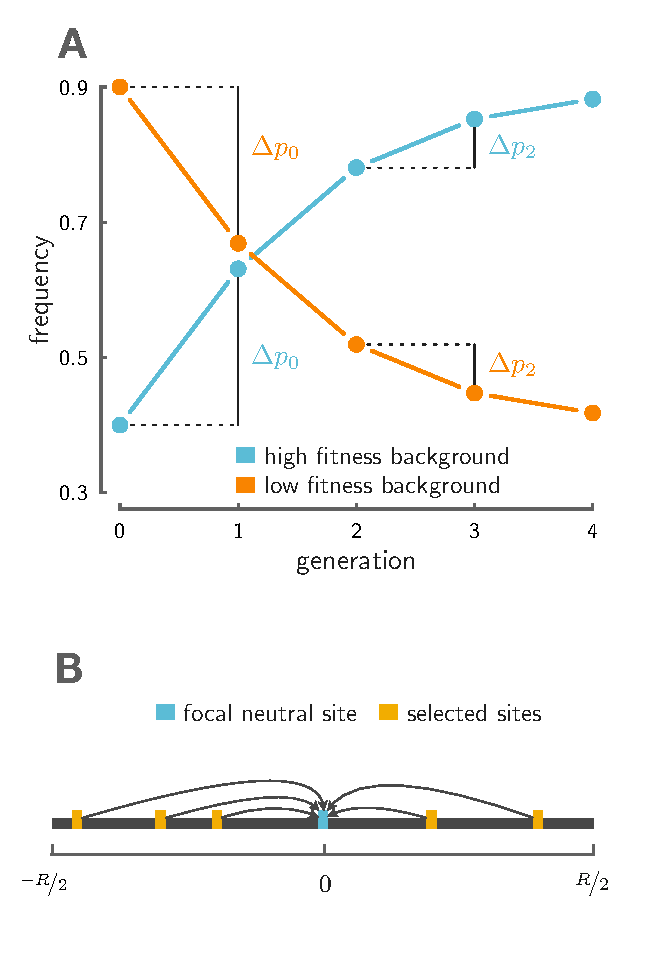
\includegraphics[width=0.5\textwidth]{./images/keynote-cartoons-figure-1.pdf}

  \caption{A: On an advantageous background (light blue), a neutral allele
    increases in frequency leading to a positive change in allele frequency
    early on, $\Delta p_0 = p_1 - p_0$. As long as some fraction of neutral
    alleles remain associated with this advantageous background, the neutral
    allele is expected to increase in frequency in later generations, here,
    $\Delta p_2 = p_3 - p_2$. This creates temporal autocovariance,
    $\cov(\Delta p_2, \Delta p_0) > 0$. Similarly, had the neutral allele found
    itself on a low-fitness background (orange), this would also create temporal
    autocovariance.  B: This depicts the setup for our multilocus model.
    Multiple alleles (yellow) determine the fitness in a region $R$ 
    Morgans in length, and these perturb the allele frequency trajectory 
    of a focal neutral site (light blue). 
  }
  \label{fig:cartoon}
\end{figure}

Temporal autocovariance is caused by the persistence over generations of the
statistical associations (linkage disequilibria) between a neutral allele and
the fitnesses of the random genetic backgrounds it finds itself on; as long as
some fraction of associations persist, the heritable variation for fitness in
one generation predicts the change in later generations, as illustrated by the
fact that $\cov(\Delta p_2, \Delta p_0) > 0$ (see Figure \ref{fig:cartoon}A).
Ultimately segregation and recombination break down haplotypes and shuffle
alleles among chromosomes, leading to the decay of autocovariance with time. 

The effect heritable variation has on neutral alleles has traditionally been
modeled in a quantitative genetics framework where a large number of loosely
linked polymorphisms contribute to heritable fitness differences between
individuals, and the impact of heritable fitness variation on a neutral allele
is quantified as a reduction in its long-run effective population size
\parencite{Robertson1961-ho,Santiago1995-hx,Santiago1998-bs}.  This form of
linked selection can be contrasted with classic population genetic hitchhiking
theory (\cite{Maynard_Smith1974-lc}), which considers how neutral alleles
closely linked to a new beneficial mutation are affected as it sweeps to
fixation. While classic population genetic linked selection models consider how
neutral variation is affected by strong associations caused by tight linkage to
an advantageous site, quantitative genetic models of linked selection
considered the weakest forms of associations: those between unlinked loci
within an individual (\cite{Morley1954-yp, Robertson1961-ho, Santiago1995-hx};
see \cite{Barton2000-zg} for more on the two models of linked selection).
\vb{These quantitative genetic models of linked selection match the expressions
  for the loss of diversity found in classic models a sweeping advantageous
  allele (p. 2110, \cite{Santiago1998-bs}) and genome-wide background selection
  (p. see equation 12 of \cite{Santiago1998-bs}, \cite{Nordborg1996-nq}).  The
distant associations considered by these models} are quickly established but
are rapidly broken down by segregation and independent assortment, yet still
can have a marked effect on diversity
\parencite{Robertson1961-ho,Santiago1995-hx}. However, since the impact of
heritable fitness variation has traditionally been modeled as causing a
reduction in the effective population size, there has been no direct way to
separately estimate its effects from those of drift. We show that with temporal
genomic data, one can directly measure the levels of temporal variances and
autocovariances of allele frequency change in the population. Additionally, we
that show temporal autocovariance is created under both tight and loosely
linked selection, and below, develop expressions for its magnitude that are
applicable to both, bridging the two regimes of linked selection.

\section{A model for multilocus temporal autocovariance}

Here, we develop theory for the temporal autocovariance in a neutral allele's
frequency changes through time, generated by the presence of heritable fitness
in the population. We measure the temporal autocovariance $\cov(\Delta p_t,
\Delta p_s)$ at a single diallelic neutral locus. Since only allele frequency
changes due to heritable variation in \emph{fitness} contribute to temporal
autocovariance, we can focus exclusively on the behavior of $\Delta_{_H} p_t$
in deriving our expressions for the autocovariance across timepoints. We
imagine that an individual $i$ has fitness $f_i$, i.e. that their expected
number of children is $f_i$. We assume a constant population size, and so the
population average fitness $\E_i(f_i) = 1$. Additionally, we assume that all
fitness variation has an additive, polygenic architecture. Then, with $L$ loci
contributing to fitness, we can write individual $i$'s fitness as $f_i = 1 +
\sum_{l=1}^L \alpha_{t,l} g_{i,l}$, where $\alpha_{t,l}$ is the effect size in
generation $t$ and $g_{i,l} \in \{0, 1, 2\}$ is individual $i$'s gene content
at locus $l$. Here, each $\alpha_{t,l}$ is analogous to a selection
coefficient acting at locus $l$, since the fitnesses for genotypes $A_1 A_1$,
$A_1 A_2$, and $A_2 A_2$ are $1$, $1 + \alpha_{t,l}$, and $1 + 2\alpha_{t,l}$
respectively. This formulation is approximately equivalent to exponential
directional selection on some additively determined trait, implying that
selection does not create linkage disequilibria between unlinked loci; see
Appendix \ref{ap:multilocus} for more detail.

When fitness variation exists in the population (that is, $\var_i(f_i) > 0$),
the frequency of the neutral allele changes stochastically, as more fit
individuals leave more descendents that inherit the neutral allele they carry
and less fit individuals leave fewer. Across the population, stochastic
associations can form between the genetic components of an individual's fitness
and the neutral allele they carry, leading the neutral allele frequency to
change due to fitness differences across individuals. The total heritable
change in neutral allele frequency $\Delta_{_H} p_t$ can then be partitioned
into each individual's contribution to this change based on their fitness $f_i$
and the number of the tracked neutral alleles they carry, $x_i \in \{0, 1,
2\}$, giving us

\begin{align}
  \Delta_{_H} p &= \frac{1}{2N} \sum_{i=1}^N x_i (f_i - 1)
\end{align}
%
\parencite{Santiago1995-hx}. Substituting each fitness $f_i$ with its genetic
basis and simplifying (see Appendix Section \ref{ap:multilocus} for
\vb{derivation and equation 10 of \cite{Kirkpatrick2002-aw}}) gives,

\begin{align}
  \Delta_{_H} p_t &=  \sum_{l=1}^L \alpha_{t,l} D_{t,l}' + \sum_{l=1}^L \alpha_{t,l} D_{t,l}'' 
\label{eq:neut-change}
\end{align}
%
where $D_{t,l}'$ is the \emph{gametic} linkage disequilibrium between the
neutral allele and the allele at the selected site $l$ on the same gamete,
whereas $D_{t,l}''$ is the \emph{non-gametic} linkage disequilibria, or the
covariance \emph{across} the neutral and selected allele on the two different
gametes forming an individual (see \cite{Weir1996-mv}, p. 121 for details and
Appendix Figure \ref{fig:ld-cartoon}A for an illustration). Intuitively, this
expression tells us that the heritable change in neutral allele frequency is
determined by the gametic and non-gametic linkage disequilibrium between the
neutral site and all sites that affect an individual's fitness, scaled by the
magnitude of each selected locus's effect. Alternatively, we can see this as
the multivariate breeder's equation, where the neutral allele is a correlated
trait responding to selection on other traits/loci \parencite{Lande1979-rq}.
This expression is the multilocus analog of the change in a neutral site's
frequency due to hitchhiking at a single linked site (see e.g. equations (2)
and (3) in \cite{Stephan2006-xz}). 

Because the effects of the non-gametic LD are relatively weak compared to the
gametic LD for tightly linked loci (see Appendix Section \ref{ap:non-gametic}
for an expression of their strength), we ignore these, and hereafter omit the
primes in our notation so that $D_{t,l}$ refers to $D_{t,l}'$.  Since
$\E(\Delta_{_H} p_t) = 0$, we can write the covariance $\cov(\Delta_{_H} p_t,
\Delta_{_H} p_s)$ as $\E(\Delta_{_H} p_t \Delta_{_H} p_s)$.  Hereafter, we also
omit the subscript $H$ since $\cov(\Delta p_t, \Delta p_s) = \cov(\Delta_{_H}
p_t, \Delta_{_H} p_s)$. Expanding these terms, the covariance between the
allele frequency changes at generations $t$ and $s$ can be written as

\begin{align}
  \cov(\Delta p_t, \Delta p_s) &=  \E \left[\left(\sum_{l=1}^L \alpha_{t,l} D_{t,l}\right) \left( \sum_{l=1}^L \alpha_{t,l} D_{s,l} \right) \right]\nnn \\ 
                               &=  \underbrace{\sum_{l=1}^L \alpha_{t,l} \alpha_{s,l} \E(D_{t,l}  D_{s,l})}_{\text{persistence of associations with selected site} \; l}  \; + 
  \underbrace{\sum_{l \ne k} \alpha_{t,k} \alpha_{s,l}\E(D_{t,k}  D_{s,l})}_{\text{cross-associations between two selected sites}}. 
  \label{eq:multilocus-twopart}
\end{align}

This statement for temporal autocovariance is fairly general, as it can handle
fluctuating selection (e.g. when $\alpha_{t,l}$ varies with time $t$) and any
additive multilocus evolution (as long the linkage disequilibria dynamics can
be specified). Looking at the first term in this sum, we see the temporal
autocovariance is determined in part by the terms $\E(D_{t,l} D_{s,l})$. These
expected LD products reflect the degree to which the association between the
neutral locus and a selected site persists from generation $t$ to $s$ (here, $t
< s$). Intuitively, the higher the initial association between the neutral and
selected loci, and the slower rate of decay of LD between sites, the greater
temporal autocovariance will be.

\subsection{The multilocus temporal autocovariance model with directional selection}
\label{sec:temp-autocov-dirsel}

Thus far, in reaching Equation \eqref{eq:multilocus-twopart} we assume only
that fitness is additive across loci. In this section, we develop a model of
how temporal autocovariance behaves specifically under directional selection
beginning at a specific time. We make three assumptions to simplify our
expressions. First, we assume that the effect size remains constant through
time, such that $\alpha_l := \alpha_{t,l}$ for all $t$ (we relax this
assumption in Section \ref{sec:fluct-sel}). Second, we ignore the contribution
of the second term of Equation \eqref{eq:multilocus-twopart}, $\E(D_{t,k}
D_{s,l})$ (for $k \ne l$), to temporal autocovariance. Under the case where the
population is initially at mutation-drift-recombination equilibrium, we expect
this product to be zero as there is no directional association between the two
selected sites and the neutral site. However, we note that interaction
  between selected sites (Hill-Robertson interference) will cause this term to
become negative \parencite{Barton2005-zq}, a point we return to later. Third,
we assume that the selected sites increase in frequency independently, such
that the dynamics of the linkage disequilibria between the neutral and selected
sites pairs can be modeled using two-locus dynamics. Using a deterministic
continuous-time model for the dynamics of the linkage disequilibrium between
the selected and neutral site \parencite{Maynard_Smith1974-lc,Barton2000-zg},
we rewrite the $\E(D_{t,l} D_{s,l})$ terms in the expression for temporal
autocovariance as

\begin{subequations}
  \begin{align}
    \cov(\Delta p_t, \Delta p_s) &= \sum_{l=1}^L \alpha_{l}^2 \E(D_{t,l} D_{s,l}) \nnn \\
                                 &= \sum_{l=1}^L \alpha_{l}^2 \E(\mathcal{R}_{t,l}^2) p_t (1-p_t) p_{s,l} (1-p_{s,l}) (1-r_l)^{s-t}  \\
    \frac{\cov(\Delta p_t, \Delta p_s)}{p_t (1-p_t)} &= \sum_{l=1}^L \alpha_{l}^2 p_{s,l} (1-p_{s,l}) \E(\mathcal{R}_{t,l}^2) (1-r_l)^{s-t}, 
  \end{align} 
  \label{eq:cov-R}
\end{subequations}
%
where $\E(\mathcal{R}^2_{t,l})$ is the square of the correlation between the
neutral site and selected site $l$ at time $t$ (a common measure of LD;
\cite{Hill1968-ue}), and $r_l$ is the recombination fraction between the
neutral site and selected site $l$.

We can further simplify this expression by assuming that there is no
covariation between the additive genic variation at a selected site and the
linkage disequilibrium between that selected site and the neutral site (see
Appendix Section \ref{ap:ml-ave-Va} for more detail). This allows us to factor
out the average additive genic variation for fitness at time $s$ and write the
covariance as

\begin{align}
  \frac{\cov(\Delta p_t, \Delta p_s)}{p_t(1-p_t) } &= \frac{V_a(s)}{2L} \sum_{l=1}^L \E(\mathcal{R}_{t,l}^2) (1-r_l)^{s-t}
  \label{eq:multilocus-cov-sum}
\end{align}
%
where $V_a(s)$ is the additive genic variance for fitness, which is the
additive genetic variance for fitness ($V_A$) without the contribution of
linkage disequilibria between selected sites, $V_a(s) = 2 \sum_l \alpha_l^2
p_l(s) (1-p_l(s))$. In part, our expression not relying on the linkage
disequilibria between selected sites is a result of ignoring the second
term in Equation \eqref{eq:multilocus-twopart}; we revisit the consequences of
this assumption further on in Section \ref{sec:ml-sim-res}.

This expression allows us to calculate the temporal autocovariance in cases
where we know the vector of recombination fractions between the neutral and
each of the selected sites, $r_1, r_2, \ldots, r_L$. Often we do not know the
exact positions of these sites, but we can treat these positions as randomly
placed on a chromosome and further simplify our model to understand the factors
that determine temporal autocovariance.

\subsection{Temporal autocovariance for an average neutral polymorphism}
\label{sec:temp-autocov-aveneut}

In the second part of our derivation, we develop a simple intuitive model of
how temporal autocovariance is determined by a few key parameters when we make
two additional assumptions. First, we assume selected sites are randomly and
uniformly distributed along the chromosome, such that a site's position on the
genetic map is a random variable $g \sim U(-\nicefrac{R}{2}, \nicefrac{R}{2})$
(where $R$ is the region's length in Morgans), and the focal neutral site with
which we calculate temporal autocovariance lies in the middle of this idealized
chromosome at the origin (as depicted in Figure \ref{fig:cartoon}B). Then, the
recombination fraction between the focal neutral site and a selected site at
random position $g$ is given by the mapping function $r(g)$, which maps the
position $g$ to a recombination fraction. A simple choice for $r(g)$ is
Haldane's mapping function, $r(g) = \frac{1}{2} (1 - e^{-2|g|})$,
(\cite{Haldane1919-qp}; note we take the absolute value of $g$ to translate the
position $g$ to a distance to the focal neutral site) and we use that here.
Second, we assume the linkage disequilibrium between each selected site and the
focal neutral site depends only the recombination fraction $r(g)$ between the
two loci, and not their absolute positions or effect sizes; then, we rewrite
$\E(\mathcal{R}^2_{t,l})$ as the function $\E(\mathcal{R}^2_t(r(g)))$. For
example, if the population was initially at drift-recombination balance, this
would be $\E(\mathcal{R}^2) = (10 + \rho)/(22 + 13 \rho + \rho^2)$ where $\rho
= 4Nr(g)$ \parencite{Ohta1969-ae,Hill1968-ue}. These assumptions allow us
  to conceptually understand the factors that determine temporal
autocovariance; in practice, in temporal studies with linkage disequilibria
data and recombination maps, one can directly calculate the sum in Equation
\eqref{eq:multilocus-cov-sum} (see Appendix Section \ref{ap:empirical-ld}). We
then write the temporal autocovariance experienced by a neutral allele in a
region $R$ Morgans long containing $V_a(s)$ fitness variation at time $s$ as

\begin{align}
  \frac{\cov(\Delta p_t, \Delta p_s)}{p_t(1-p_t) } &\approx \frac{V_a(s)}{2 R} \int_{-\nicefrac{R}{2}}^{\nicefrac{R}{2}} \E(\mathcal{R}_t^2(r(g))) (1-r(g))^{(s-t)} \,dg
  \label{eq:ave-neut-autocov}
\end{align}
%
(see Appendix Section \ref{ap:ml-cont} for details).

This integral is the sum of the initial LD between a typical neutral locus and
selected site, weighted by the decay of LD due to recombination over $s-t$
generations. Selection enters here through the total additive genic variance
for fitness for the region divided by the genetic map length of the region
($\nicefrac{V_a(s)}{R}$). Thus a key compound parameter in describing the
temporal covariance is the additive genic variance per Morgan, a quantity
somewhat similar to the ratio of new adaptive mutations per basepair to
recombination per basepair, $\nicefrac{\nu_\text{BP}}{r_\text{BP}}$, that
occurs in models of recurrent sweeps \parencite{Stephan1992-jc} and models of
the limits of selection with linked loci
\parencite{Robertson1970-xk,Robertson1976-la}. \vb{Note that this does not
  include the effects of genome-wide fitness variation, e.g. the impact
  unlinked selected sites have on the neutral site due to the associations
created when the sites sort within the same individuals. We quantify the
magnitude of these in Appendix \ref{ap:unlinked-contribution}}.

%GRAHAM'S ALT VERSION
 % Imagine that an average base
 % pair of DNA contributes $V_{a,bp}(s)$ to the genic variance, and
%  $r_{BP}$ to the total recombination rate, then this compound
%parameter will be $\nicefrac{V_{a,bp}(s)}{r_{BP}}$. Thus the
%temporal covariance is determined by the }

To validate our theory, we simulate a fixed region of $R$ Morgans and
calculate the covariance in allele frequency changes by averaging over many
uniformly distributed neutral sites within this region. Then, the random
distance between a neutral site's position $n$ and a selected site's position
$g$ is $c = |n - g|$, where $n, g \sim U(0, R)$; this random variable $c$ has a
triangle distribution, $f(c) = 2(R-c) / R^2$. Averaging over the positions of
both randomly placed neutral and selected sites, the temporal autocovariance
is

\begin{align}
  \label{eq:multilocus-triangle}
  \Sigma_{t,s} := \frac{\E_n(\cov(\Delta p_t, \Delta p_s))}{\E_n(p_{t} (1-p_{t}))} &= \frac{V_a(s)}{2} \underbrace{\int_0^R \E(\mathcal{R}_t^2(r(c))) \; (1-r(c))^{(s-t)} \frac{2(R-c)}{R^2} \,d c}_{\mathcal{A}(R, t, s)} 
\end{align}
%
where $\E_n(\cdot)$ indicates an expectation taken over the position of the
randomly placed neutral sites, and we define $\mathcal{A}(R, t, s)$ as the
average linkage disequilibrium between selected and neutral sites that persists
from generations $t$ to $s$ ($t \le s$). As is common with estimating the
expected values of other ratios like $F_{ST}$ \parencite{Bhatia2013-zy}, we use
a ratio of expectations rather than the expectation of the ratio.

We can also use this expression to calculate the variance of allele frequency
change. The standardized variance $\nicefrac{\var(\Delta p_t)}{p_t(1-p_t)}$ has
two components: the drift term and the heritable variance in offspring number.
Adding these independent contributions, the standardized variance is

\begin{align}
  \frac{\E_n(\var(\Delta p_t))}{\E_n(p_t(1-p_t))} = \frac{V_N + 2}{8N} + \frac{V_a}{2} \mathcal{A}(R, t, s)
  \label{eq:multilocus-var}
\end{align}
%
where $V_N$ is the non-heritable variance in offspring number. Under a
Wright--Fisher model of reproduction, $V_N \approx 2$, this simplifies to

\begin{align}
  \Sigma_{t,t} := \frac{\E_n(\var(\Delta p_t))}{\E_n(p_t(1-p_t))} = \frac{1}{2N}  + \frac{V_a}{2} \mathcal{A}(R, t, s).
  \label{eq:multilocus-var-2}
\end{align}

When combined, this expression for the variance in allele frequency change and
our expression for temporal autocovariance are in agreement with Robertson
(\citeyear{Robertson1961-ho}) and Santiago and Caballero
(\citeyear{Santiago1995-hx, Santiago1998-bs}) when predicting the total
variance in allele frequency change; see Appendix \ref{ap:connecting-sc}.
With the above expressions for the variances and covariances, we have a
  complete set of theoretical expressions for the variance-covariance matrix of
  allele frequency change, which we call $\mathbf{\Sigma}$, with the diagonal
  variance elements $\Sigma_{t,t}$ given by Equation \eqref{eq:multilocus-var-2},
  and the upper- and lower-triangle covariance elements $\Sigma_{t,s}$ ($t \ne
  s$) given by Equation \eqref{eq:multilocus-triangle}.

\subsection{Modeling the dynamics of additive genic and genetic variation}
\label{sec:dyn-var}

Our expressions for temporal autocovariance (Equation
\ref{eq:multilocus-triangle}) requires an expression for $V_a(t)$, the additive
genic variation through time.  However, we lack general expressions for the
dynamics of the additive genic variation during selection, as these dynamics
are quite complex for a few reasons. First, since our theory considers
polygenic selection at a finite number loci in a region, additive genic
variation is not constant as it would be under an infinitesimal model
\parencite{Bulmer1980-zo}. Second, we allow for arbitrary levels of
recombination from very tight linkage to loose linkage.  Previous work has
shown that predicting the dynamics of additive genic variation in a system with
an arbitrary level of recombination is difficult, as both the additive genic
and genetic variances depend on the higher-order moments of linkage
disequilibrium (see \cite{Barton1987-gl}, and p. 607 of \cite{Turelli1990-kd}). 

A primary determinant of the additive genic variation is the heterozygosity of
the selected sites. Assuming effect sizes are constant through time and across
loci, we can rewrite the additive genic variation, $V_a(t) = 2 \alpha^2 \sum_l
p_l(t) (1-p_l(t))$, as

\begin{align}
  \label{eq:VA-SSH}
  V_a(t) &= \alpha^2 SSH(t) \\
  V_a(t) &= V_a(1) \frac{SSH(t)}{SSH(1)}
\end{align}
%
where $SSH(t) = 2 \sum_l p_l(t) (1-p_l(t))$ is the sum of site heterozygosity
at time $t$.  Ideally, we would directly use $SSH(t)$ in a region; however,
this would require knowing \emph{a priori} which sites are being selected.
Instead, we assume that the trait is sufficiently polygenic that frequency
changes due to selection are weak, and that the change in heterozygosity at
neighboring neutral polymorphic sites approximately mirrors that at selected
polymorphisms \vb{(this is the case under the infinitesimal model, where the
change in frequencies due to selection is no different than the change due to
drift; \cite{Bulmer1980-zo,Robertson1960-jz}, \cite{Kimura1984-ia}, Ch.6)}.
Then, using the sum of site heterozygosity at neutral sites, $SSH_n(t)$, as a
proxy for the sum of site heterozygosity at selected sites, 

\begin{align}
  V_{a,ssh_n}(t) := V_a(1) ssh_n(s)
  \label{eq:VA-ssh}
\end{align}
%
where we define $ssh_n(s) = \nicefrac{SSH_n(s)}{SSH_n(1)}$ as the factor by
which $V_a(1)$ decreases at time $s$, approximated by neutral sites' allele
frequency changes. Under this approximation, the dynamics of genic variation
are determined by one free parameter, $V_a(1)$, and the directly measurable sum of
site heterozygosity at neutral sites through time. 

Our focus here is on the short-term response of a population, and so we look at
the decay of genetic backgrounds present at the onset of directional selection.
In reality, new mutations consistently create additive genetic variation for
fitness; thus, an equilibrium level of additive genetic variance in the
population can be maintained. The long-run effect of linked selection under
this equilibrium model is handled by
\textcite{Santiago1995-hx,Santiago1998-bs}; see Appendix
\ref{ap:connecting-sc}.

\subsection{Multilocus Simulation Details}
\label{sec:ml-sim}

To test our theoretical expressions, we have conducted extensive forward
simulations of directional selection on a polygenic trait. We vary four
critical parameters in these simulations: (1) the level of additive genetic
variance at the onset of selection ($V_A$), (2) the level of recombination ($R$
in Morgans), (3) the number of selected sites in the region ($L$), and (4) the
population size ($N$). We choose our grid of the selection and recombination
parameters based on the levels we would expect across a wide variety of
organisms; see Appendix Section \ref{sec:supp-ml-sim-param} for details. We
used three different population sizes ($N \in \{100, 500, 1000\}$), but note
that we use $N=1000$ and a subset of the other parameters in our figures.

%with $V_a \in \{0.001, 0.002, 0.005, 0.01,
%0.02, 0.05, 0.08, 0.1\}$, $R \in \{0, 0.005, 0.01, 0.05, 0.1, 0.5, 1.5, 4.5\}$,
%and $L \in \{10, 50, 100, 500\}$ (see \ref{sec:supp-ml-sim-param} for details;
%note that we use $N=1000$ and a subset of the other parameters in our figures
%to prevent overplotting).

Before the onset of selection, we create the initial diploid population from a
pool of gametes created by \texttt{msprime} \parencite{Kelleher2016-oi}, such
that the initial allele frequency distribution and linkage disequilibria
between sites is at mutation-drift-recombination balance. Details of how
\texttt{msprime} was called are available this paper's code repository
(\url{https://github.com/vsbuffalo/tempautocov}), in \texttt{R/simpop.r}. Then, we
pass this pool of gametes into a forward Wright--Fisher-with-recombination
simulation routine and let it evolve for four generations neutrally before
initiating selection on the fifth generation.  These first four generations of
neutral evolution (without mutation) serve as a control to validate that the
variance in neutral allele frequency change is as expected under a
Wright--Fisher model and that temporal autocovariance between a generation
before selection and during selection is zero.

We generate genetic variation for fitness by choosing $L$ random loci from the
neutrally evolved sites, and randomly assign an effect size of $-\alpha$ or
$+\alpha$, such that the expected total amount of additive genic variation is
$V_A$ (note that the initial additive genic and genetic variance are equal,
$V_A = V_a$, as the LD contribution is zero for randomly chosen sites). The
details of this are given in Appendix Section \ref{sec:supp-ml-sim-va}. This
approach creates some additional variance around the target level of additive
genic variation, as the sum of site heterozygosities will vary stochastically
across simulation replicates. At the onset of selection, an individual $i$'s
trait value is calculated as $z_i = \sum_{i=1}^L \alpha g_{i,l}$ where
$g_{i,l}$ is their number of alleles with effect size $\alpha$ at locus $l$.
Then, their absolute fitness is calculated using an exponential fitness
function $w(z_i) = e^{z_i}$ (\cite{Turelli1990-kd}, p. 17). Under our
Wright--Fisher model, we sample the parents of the next generation according to
a multinomial distribution, where the probability of individual $i$ being a
parent is $\nicefrac{w(z_i)}{\bar{w}}$. 

We record 50 generations of simulated evolution, after which we compute
the standardized sample temporal variance-covariance matrix $\mathbf{Q}$
(this is the sample analog of our theoretical variance-covariance matrix
$\mathbf{\Sigma}$), for each replicate as follows. First, we mark
frequencies reaching fixation or loss as missing values. This allows the
  frequency changes before fixation/loss to contribute to the measured
  covariance, rather than removing the entire locus's trajectory, which would
  act to condition the covariance on more intermediate frequencies. Note that
  one cannot ignore fixations or losses, as these have $\Delta p_t=0$ and thus
  an autocovariance of zero, which would act to underestimate the true level of
autocovariance at segregating sites. Having marked fixations/losses as missing,
we take the frequency matrix and calculate a vector of allele frequency
changes $\Delta \vec{p}_n = [\Delta p_{n,1}, \Delta p_{n,2}, \ldots, \Delta
p_{n,\tau}]$ using each neutral locus $n$'s $\tau+1$ observed generations.
Finally, we calculate the $\tau \times \tau$ sample standardized
variance-covariance matrix $\mathbf{Q}$, averaging over $M$ neutral loci such
that element $Q_{t,s}$ is calculated as

\begin{align}
  Q_{t,s} = \frac{\frac{1}{M - 1} \sum_{n=1}^M \left( \Delta p_{n,t} \Delta p_{n,s} - \left(\frac{1}{M} \sum_{n=1}^M \Delta p_{n,t}\right) \left( \frac{1}{M} \sum_{n=1}^M \Delta p_{n,s} \right) \right)}{
  \frac{1}{M} \sum_{n=1}^M p_{\min(t,s)} \left(1 - p_{\min(t,s)}\right)
  },
  %\frac{\cov_n(\Delta p_s, \Delta p_t)}{\E_n\left(p_{\min(s,t)} (1-p_{\min(s,t)}\right)}
  \label{eq:ave-temp-autocov}
\end{align}
%
though see Appendix Section \ref{sec:sampling} for a bias-corrected version
when sample, rather than population allele frequencies are used. Sums over
missing values only use pairwise-complete observations, implemented by R's
\texttt{cov()} function's \texttt{use='pairwise.complete'} argument.

We have extensively validated our simulation procedure in a neutrally evolving
population, ensuring that the decay of linkage disequilibrium and the allele
frequency change match expectations (see Supplementary Figures
\ref{fig:het-neut}, \ref{fig:ld-neut}, and \ref{fig:ne-neut}). 


\subsection{Comparing theory to simulation results}
\label{sec:ml-sim-res}

To validate our expressions for temporal autocovariance, we compare the levels
of autocovariance and variance predicted by Equation
\eqref{eq:multilocus-triangle} and \eqref{eq:multilocus-var-2} to the average
levels observed across simulation replicates. To calculate the theoretical values
of temporal autocovariance and variance, our expression requires the additive
genic variation at $s$, $V_a(s)$; however, as described in Section
\ref{sec:dyn-var}, we lack an analytic expression for the dynamics of genic
variation to plug into $V_a(s)$.  Following the approach of others in
evolutionary quantitative genetics (\cite{Turelli1994-rd}, p. 930), we
substitute the numerical values calculated directly from the simulation data
for $V_a(s)$. Additionally we consider two other numerical values related to
the additive genic variance: the observed additive genetic variance from our
simulations ($V_A(s) = \var_i(z_i)$ at time $s$, which includes the
contribution of LD between selected sites), and the additive genic variation at
time $s$ as approximated by the observed decay in the sum of site
heterozygosity at neutral sites ($V_{a,ssh_n}(1)$, as described in Section
\ref{sec:dyn-var}). 

\begin{figure}[!ht]
  \centering
  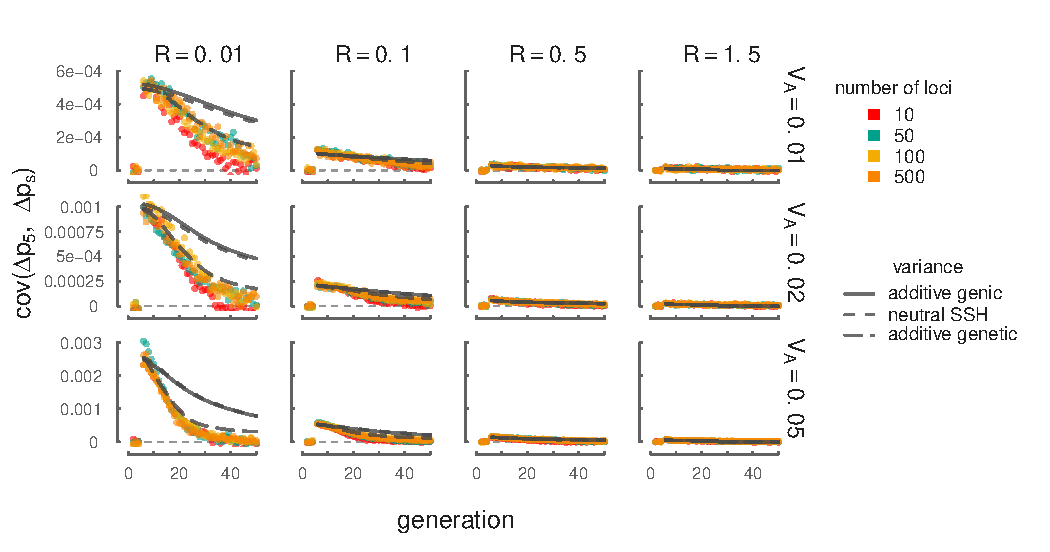
\includegraphics{./images/sim-pred-covs-varyl-alt.pdf}

  \caption{ In each panel the temporal autocovariance $\cov(\Delta p_5, \Delta
    p_s)$ is shown on the y-axis while generation $s$ varies along the x-axis.
    Selection is initiated on the $5^\text{th}$ generation, so $\Delta p_5$ is
    the neutral allele's frequency change across the first generation of
    selection. Each point is the temporal autocovariance between $\Delta p_5$
    and the $\Delta p_s$ in a region, averaged over 100 simulation replicates,
    with the colors indicating the number of selected loci. The gray curves
    indicate the theoretical predictions (for $L=500$ loci only) using Equation
    \eqref{eq:multilocus-triangle}, with the equation's variance provided by
    the empirically observed additive genic (solid), the additive genetic (long
    dashes), and the neutral sum of site heterozygosity approximation (short
    dashes). A thin horizontal dashed line indicates $y=0$.  Across the
    columns, the level of recombination (in Morgans) is varied; across rows,
    the initial level of additive genetic variation is varied.  Note that while
    our results here are between the frequency change at the onset of selection
    $\Delta p_5$ and some later change $\Delta p_s$, our covariance theory
    matches simulation results between any two arbitrary frequency changes
  $\Delta p_t$, and $\Delta p_s$; see Supplementary Figure
\ref{fig:multilocus-expfit-sims-gen13}.}

  \label{fig:multilocus-expfit-sims}
\end{figure}

Figure \ref{fig:multilocus-expfit-sims} compares the fit of our theory with
differing additive genetic variances with the empirical
covariances from our multilocus simulations. In each panel, we plot the level
of temporal autocovariance between the allele frequency change across the first
two generations of selection ($\Delta p_5$) and some later allele frequency
change $\Delta p_s$ where $s$ varies along the x-axis. Each point represents
the temporal autocovariance (calculated across all sites in a region according
to Equation \ref{eq:ave-temp-autocov}) averaged across 100 replicate
simulations, with the color of the point indicating the number of selected
sites in the region. Within each panel, the temporal autocovariance predicted
by Equation \eqref{eq:multilocus-triangle} is plotted as a set of three
lines, one for each of the three different types of variance we have
substituted in for $V_a(s)$. Overall, the fit is close but varies depending on
the type of variance used for $V_a(s)$; we discuss each in turn below.

Using empirical additive genic variation (solid lines), our theory provides a
good fit to the simulation results for a short period after selection is
initiated ($\sim$5 generations) in regions with tighter linkage ($R=0.01$
Morgans) across a range of additive genetic variation parameters ($0.01 \le V_A
\le 0.05$; see Supplementary Figure \ref{fig:multilocus-expfit-sims-va-oom} for
$V_A$ varying over orders of magnitude). With looser linkage ($R \ge 0.1$
Morgans), our theory using the empirical additive genic variation fits much
more closely over a longer duration ($\sim$10-15 generations). Note that some
variability is caused by the noise of each simulation replicate around the
target initial additive genetic variation $V_a$ (see Section \ref{sec:ml-sim}),
as each replicate samples sites from a neutral coalescent. Our theory also
accurately predicts the temporal autocovariance for different choices of
reference generation, i.e.  varying $t$, see Supplementary Figure
\ref{fig:multilocus-expfit-sims-gen13}.

When we use the sum of site heterozygosity at neutral sites ($V_{a,ssh_n}$,
shown as a short-dashed lines) as a proxy for additive genic variation, the
theory fits simulations over the same timespan as using the empirical additive
genic variation. This is because (1) the SSH at neutral sites closely matches
the SSH at selected sites, and (2) both closely follow the dynamics of additive
genic variation through time (see Supplementary Figure
\ref{fig:multilocus-expfit-vark}). Using $V_{a,ssh_n}$ has the advantage that
we can directly measure neutral SSH, which proves useful later in Section
\ref{sec:meth-moments}, as we use this approach to help infer the initial
additive genic variation at the onset of selection.

Finally, we find using the additive genetic variance $V_A(s) = \var_i(z_i)$
accurately predicts the dynamics of temporal autocovariance over tens of
generations (see the long-dashed lines in Figure
\ref{fig:multilocus-expfit-sims}). Furthermore, calculating the temporal
autocovariance using the empirical additive genetic variation better fits
simulation data in regimes with tight recombination, where using genic
variation performs poorly after the first few generations (e.g. the column of
panels where $R=0.01$). Thus using the additive genetic variance in our
framework provides a good fit to the temporal dynamics over relatively long
time spans.

What differentiates $V_A(s)$ from $V_a(s)$ that could explain this better fit?
The additive genic variation $V_a(s)$ ignores the contribution of linkage
disequilibria between selected sites. We can write the additive genetic
variance as

\begin{align} V_A(s) = \var_i(z_i, s) = \underbrace{2 \alpha^2 \sum_{l=1}^L
p_{l}(s) (1-p_{l}(s))}_{\text{genic variation}, \; V_a(s)} +
\underbrace{\alpha^2 \sum_{i\ne j} D_{i,j}(s)}_\text{LD contribution }
\label{eq:var-genic-z} \end{align}
%
where $D_{i,j}(s)$ is the LD between selected sites $i$ and $j$ at time $s$.
At the onset of selection, there is no expected linkage disequilibria between
selected sites since the sites and effect sizes were randomly sampled --- in
other words, $\E(D_{i,j}(s)) = 0$. We see this in Figure
\ref{fig:multilocus-expfit-sims}, as the temporal autocovariance predicted with
$V_a(s)$ match those of $V_A(s)$ when $s = 6$ (see also Supplementary Figure
\ref{fig:multilocus-expfit-vark}, which plots the empirical additive genic and
genetic variances over time). Over time, these two quantities diverge as
negative linkage disequilibria build up. While negative linkage disequilibria
between selected sites build up due to epistasis under some forms of selection
(known as the Bulmer effect, \cite{Bulmer1971-ae,Bulmer1980-zo}), this is known
not to happen under multiplicative selection (\cite{Burger2000-an}, p. 50, 177)
that is equivalent to the exponential directional selection fitness surface we
have used in our simulations. Instead, the build up of negative linkage
disequilibria between selected sites is likely due to Hill-Robertson
interference (HRi) between selected sites \parencite{Hill1966-kd}, which
affects the total additive genetic variation that selection is acting on. HRi
refers to the creation of negative LD among beneficial alleles in finite
population resulting from the fact that beneficial alleles that are on the same
haplotype move more quickly through the population than beneficial alleles on
deleterious backgrounds, resulting in negative LD.  This negative LD among
beneficial alleles lowers $V_A$ compared to the genic $V_a$
\parencite{Hill1966-kd,Barton2005-zq,Crouch2017-xr,Good2014-yz}. In the
derivation of our expression for temporal autocovariance, we greatly simplified
the multilocus dynamics by ignoring the second term in Equation
\eqref{eq:multilocus-twopart}. This term includes the expected product of two
LD terms; each is the LD between the neutral site and a selected site. Using
full multilocus theory, one may find that by including these LD products, that
$V_A$ rather than $V_a$ factors out the expression in Equation
\eqref{eq:cov-R}, but we leave this for future work. Importantly, our
simulation results suggest that the negative linkage disequilibria created by
selective interference only affects the temporal autocovariances through the
variance term $V_a(s)$, and that the actual variance determining temporal
autocovariance is the additive genetic variance, $V_A(s)$.

% \vb{Should we include mention of HRi / N, AND mention the measured negative LD?}
%\paragraph{Total variance in allele frequencies} 
% \vb{COMMENTED OUT paragraph header -- hesitant to have this be the only paragraph header in main paper -- really needed?}

In addition to modeling autocovariance through time, our theory can predict the
total temporal variance in allele frequency, $\var(p_t - p_0)$, when there is
heritable variation for fitness. Furthermore, from Equation
\eqref{eq:var-decomp} recall that we can decompose $\var(p_t - p_0)$ into
variance and covariance components. The variance components are determined by
both the magnitude of drift ($\nicefrac{1}{2N}$) and selection according to
Equation \eqref{eq:multilocus-var}, and the covariance components are
determined solely by selection according to Equation
\eqref{eq:multilocus-triangle} (assuming no inheritance of environmental
factors). Using our theory, we have predictions for each of these components
given the amount of additive genic/genetic variation for fitness, the
population size ($N$), and the amount of recombination ($R$). In Figure
\ref{fig:multilocus-expfit-cumcov}, we compare the magnitudes of these
components (averaged over the replicates of our simulations) to our theoretical
predictions. We depict the predictions for the variance and covariance
components using both the empirical additive genetic variance ($V_A$) and the
neutral sum of site heterozygosity proxy ($V_{a,ssh_n}$) as adjacent bars, each
around a point range with the point representing the average value over
simulation replicates, and the bars indicating the lower and upper quartiles
over simulations. 

\begin{figure}[!ht]
  \centering
  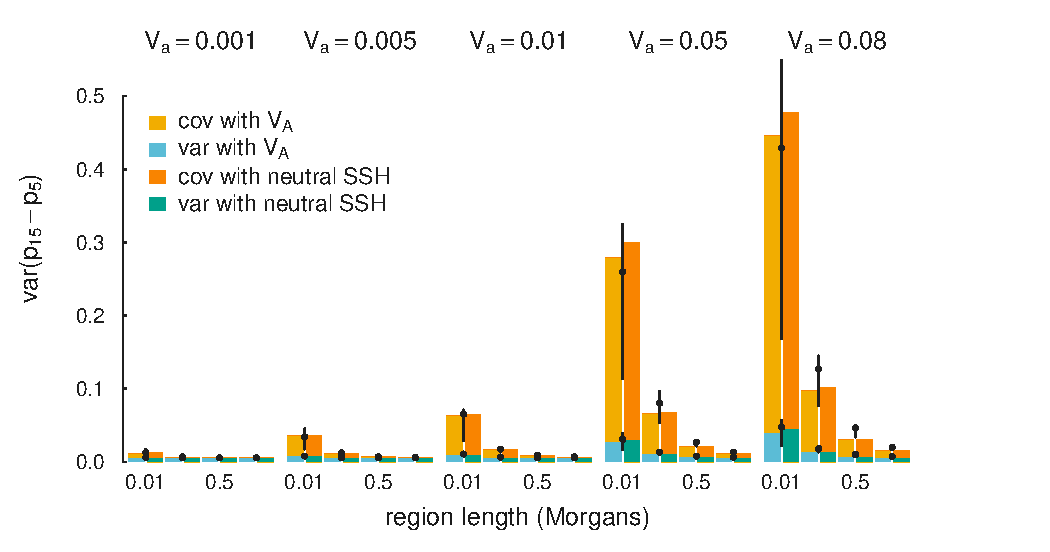
\includegraphics{./images/cummulative-cov-var-all.pdf}

  \caption{Summing over generations, Equations \eqref{eq:multilocus-twopart}
    and \eqref{eq:multilocus-var-2} accurately predicts the total variation in
    allele frequency change due to variance and covariance components. The
    predicted cumulative variance in allele frequency change across the ten
    generations after selection ($\var(p_{15} - p_5)$) is shown as bars, using
    both the empirical additive genetic variation $V_A$ (bars to the left of
    the pointrange), and the empirical neutral sum of site heterozygosity (bars
    to the right of the pointrange). The variance and covariance components are
    represented by blue/green and orange/yellow tones respectively. Finally, we
    show the averaged results of our simulations as pointranges, with the point
  depicting the average and the bars representing the lower and upper
quartiles.} \label{fig:multilocus-expfit-cumcov}

\end{figure}

Finally, we have found that across a wide range of recombination and additive
genetic variation parameters, the temporal autocovariance $\cov(\Delta p_t,
\Delta p_s)$ is largely determined by the compound parameter $\nicefrac{V_A}{R}$
and the number of generations between $t$ and $s$, which is a factor in
Equation \eqref{eq:ave-neut-autocov}. We show in Figure
\ref{fig:multilocus-va-r} that the temporal autocovariance $\cov(\Delta p_5,
\Delta p_s)$ from simulations across a wide range of $V_A$ and $R$ parameters
fall roughly on the same curve for each number of elapsed $s-t$ generations.


\begin{figure}[!ht]
  \centering
  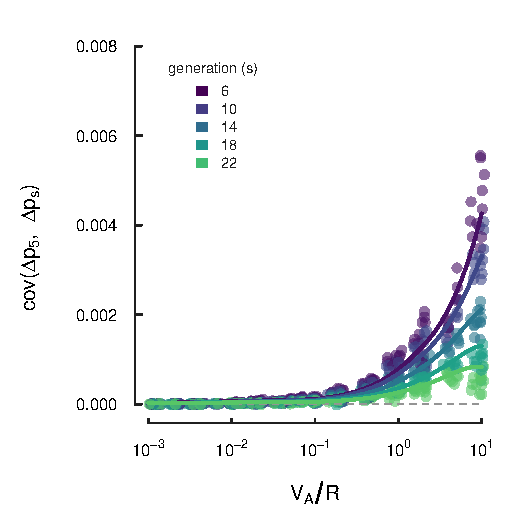
\includegraphics{./images/va-r-cov.pdf}
  \caption{The compound parameter $\nicefrac{V_A}{R}$ and the number of
    generations between the temporal autocovariance $s-t$ largely determines the
    magnitude of the temporal autocovariance across a wide spectrum of $V_A$
    and $R$ parameters. Each point is a simulation replicate with its x-axis
  position given by $\nicefrac{V_A}{R}$, the y-axis position equal to the
  temporal autocovariance, and the number of elapsed generations ($s-t$). Each
  line is a loess curve fit through each set of points for a particular generation
(with smoothing parameter $\alpha = 0.9$).}

\label{fig:multilocus-va-r}
\end{figure}

\section{Estimating linked-selection parameters from temporal autocovariance}  
\label{sec:meth-moments}

Our multilocus theory provides analytic expressions for the expected variances
and covariances of a neutral allele's frequency; thus a natural approach to
parameter estimation is to equate these expectations to averages from the data
and apply the method-of-moments. We describe a method-of-moments procedure
below to estimate the initial additive genetic variance at the onset of
selection ($V_A(1)$) in the first generation, and the drift-effective
population size ($N$) from temporal data within a single region $R$ Morgans
long, and then show a simple extension that allows this to be applied to
genome-wide data. Our basic approach is to calculate first the sample variances
and covariances of the $\tau$ observed generation-to-generation allele
frequency changes, averaging over all of the putatively neutral sites in a
region. We then equate these sample variances and covariances to our analytic
expressions for the variance and covariances, leaving us with an overdetermined
system of equations, which we solve using least squares. We demonstrate that this
simple estimation procedure provides accurate estimates of initial additive
genetic variance and the drift-effective population size. We focus on this
  procedure, as it is simple and handles  incomplete trajectories due to
  missing data or fixation/loss well. Calculating pairwise-complete covariances
  can leave sample covariances matrices non-positive definite, which makes
  maximum likelihood estimation perhaps much more difficult. Throughout, we use
  population allele frequencies (i.e.  there is no sampling noise) which
  simplifies the description of the method; in Appendix Section
  \ref{sec:sampling} we describe how the method is changed by finite sampling
  of chromosomes from a population. 

From our multilocus theory, we have analytic expressions for each element of
the $\tau \times \tau$ covariance matrix of allele frequency changes in a
region. To model the additive genic variance through time, we use the empirical
neutral sum of site heterozygosity approximation as described in Section
\ref{sec:dyn-var}. This approximates the rate that the additive genic variation
decreases through time from some initial level, $V_A(1)$, which we wish to
estimate. In total, we have $\tau + \nicefrac{\tau(\tau-1)}{2}$ unique moment
equations, which for the variance and covariance are defined as

\begin{align}
  % \E(\Delta p_t) &= 0 \\
  \frac{\var(\Delta p_t)}{\E(p_t ( 1- p_t))} \; \; &= \; \;
                                                     \frac{\widehat{V_A(1)}}{2}
                                                     \frac{\nssh(t)}{
                                                     \nssh(1)}
                                                     \mathcal{A}(R, t,t)
                                                     + \widehat{F} \;\; :=  \;\; \Sigma_{t,t}  \label{eq:mom-moments-var} \\
  \frac{\cov(\Delta p_t, \Delta p_s)}{\E(p_{t} (1-p_{t}))} \;\; &= \;\; \frac{\widehat{V_A(1)}}{2}\frac{\nssh(s)}{ \nssh(1)} \mathcal{A}(R, t,s) \;\; := \;\; \Sigma_{t,s} \; \; (\text{for} \; s > t ).
 \label{eq:mom-moments-cov}
\end{align}
%
Here the first line gives the form of $\tau$ equations for the variance of
allele  frequency changes between subsequent generations, which includes the
effect of genetic drift, $\widehat{F} =\nicefrac{1}{2N}$. The second line gives
the form of the covariances of allele frequency changes among different
generations. The term $\mathcal{A}(R, t,s)$ is the average level of linkage
disequilibrium after the $s-t$ generations that have elapsed, given there are
$R$ Morgans of recombination. In our multilocus theory section and simulations,
this is equal to the integral in Equation \eqref{eq:multilocus-triangle}.
However, we can also directly calculate a sample $\overline{\mathcal{A}(R,
t,s)}$ from observed linkage disequilibrium in a region (for details, see
Appendix Equation \eqref{eq:supp-emp-assoc}).

Following the method-of-moments, we equate each of these independent $\tau +
\nicefrac{\tau(\tau-1)}{2}$ equations for $\Sigma_{t,s}$ to the observed
sampling moments, the elements $Q_{t,s}$ of the upper triangle of the observed
heterozygosity-normalized covariance matrix $\mathbf{\widehat{Q}}$ described in
Equation \eqref{eq:ave-temp-autocov}. This yields $\tau + \nicefrac{\tau (\tau
- 1)}{2}$ equations with 2 unknown parameters: $\widehat{V_A(1)}$ and
$\widehat{N}$. We solve this overdetermined system of equations using least
squares, an approach similar to the generalized method-of-moments in
econometrics \parencite{Hansen1982-ck}. This approach finds parameter estimates
that minimize the squared error between the moment-based parameter estimate and
the true parameter value, with respect to the true parameter value. We write
the elements $Q_{t,s}$ of the upper triangle of the observed covariance matrix
in the vector $\vec{q}$, and write the method-of-moments equations as,

\begin{align}
 \vec{q} &= \widehat{V_A(1)} \vec{a} + \widehat{F} \vec{b} + \vec{\varepsilon}  
 \label{eq:mom-regression} 
\end{align}
where the elements of $\vec{a}$  and $\vec{b}$, in the same order as $\vec{q}$, are given by
\begin{align}
  a_{t,s} &= \frac{1}{2}\frac{\nssh(s)}{\nssh(t)}\mathcal{A}(R, t,s),~ b_{t,s} = \delta_{t,s}
\end{align}
%
where $\delta_{t,s}$ is an indicator variable that is $1$ when $s=t$
and zero otherwise.

Then, we can readily estimate the parameters $\widehat{V_A(1)}$ and
$\widehat{F}$ using least squares. We then obtain an estimate of $\widehat{N}$
by taking $\nicefrac{1}{2\widehat{F}}$. Since these equations are not
statistically independent, we cannot assume $\cov(\vec{\varepsilon}) = \sigma^2
\mathbf{I}$. However, this does not affect our estimates $\widehat{V_A(1)}$ and
$\widehat{F}$, as the least squares procedure is unbiased regardless of the
covariance structure between the error terms \parencite[p.
26]{Christensen2011-cg}.


Using this method-of-moments approach, we sought to infer the parameters of 20
of the replicates across the 254 parameter combinations (the same as used in
Figure \ref{fig:multilocus-expfit-sims}). We use the first five generations
after the onset of selection to infer $\widehat{V_A(1)}$ and $\widehat{N}$, as
for this short timespan the additive genetic variance is well approximated
using sum of neutral site heterozygosity approach (see Section
\ref{sec:ml-sim-res}). Each simulation replicate includes around 500 neutral
sites (the exact number is random, see Appendix \ref{sec:supp-ml-sim-param} for
details).

Applying our approach to these simulations, we find we can infer both the
initial level of additive genetic variation $V_A(1)$, and the effective
population size $N$ from multilocus temporal data. In Figure
\ref{fig:mom-fits-both}A, we show that our method-of-moments gives reasonable
estimates for the initial level of additive genetic variance over orders of
magnitude of additive genetic variation, and different recombination regimes.
As additive genetic variation for fitness becomes weaker (the left side of the
figure), our estimates become more noisy. In Figure \ref{fig:mom-fits-both}B we
show the simultaneously estimated population size $N$ against the true
population size value. We also plot the estimated $N_e$ (not accounting for
selection) from a simple temporal estimator, $N_e = -t / (2 \log(1-F))$
\parencite{Krimbas1971-et,Waples1989-sj} where $F$ is Wright's standardized
variance \parencite{Wright1931-fl}. While with high $V_A$ and low $R$, the
method-of-moments approach still underestimates $N$, it performs far better
than a standard temporal $N_e$ estimator that does not account for selection.
In Appendix Figure \ref{fig:mom-fits-both-finite}, we include a version of this
figure calculated using the method of moments on sample allele frequencies for
a sample of size $n=100$ chromosomes.

\begin{figure}
  \centering
  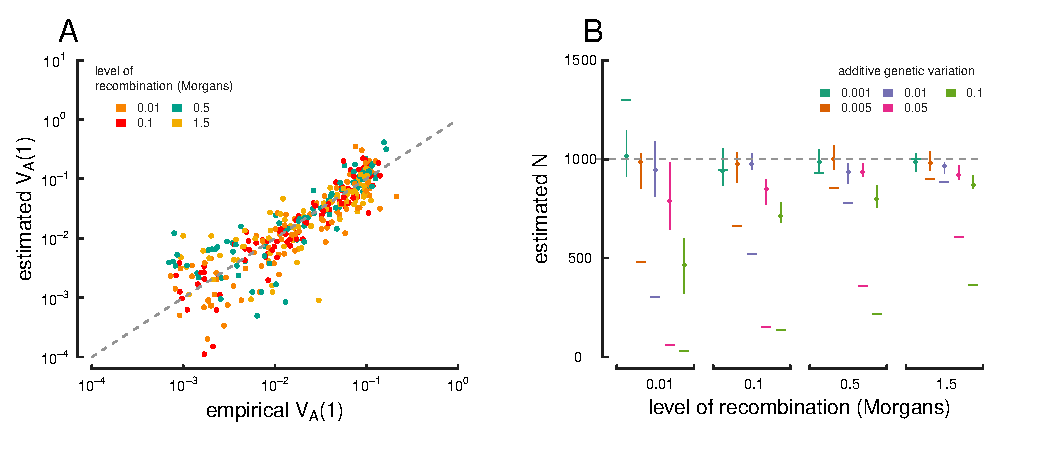
\includegraphics{./images/mom-fits-both-alt.pdf} 

  \caption{True parameter values and estimates using the method-of-moments
    approach on multilocus simulation data. (A) The true $V_A(1)$ (x-axis) and
    $\widehat{V_A(1)}$ estimated from the variance/covariance matrix (y-axis)
    for each simulation replicate across different levels of recombination
    (indicated by each point's color). The dashed gray line shows the $y=x$
    line where an estimate is exactly true to its real value. Note that the
    plot is on a log-log scale, as $V_A$ varies across orders of magnitude in
    our simulations. (B) Estimated drift-effective population size
    ($\widehat{N}$) across a range of simulations with different levels of
    additive genetic variance and recombination. Each point denotes the median,
    with lines denoting the interquartile range. A simple temporal estimate of
    the effective population size, estimated accounting for the effects of
    selection, is averaged for each replicate and plotted as a dash.  The true
    value ($N = 1,000$) is shown with the dashed gray line. Population
    frequencies (without sampling noise) are used in this figure; see Appendix
    Figure \ref{fig:mom-fits-both-finite} for an analogous figure calculated
    with sample frequencies.}

\label{fig:mom-fits-both}
\end{figure}

We can extend this approach to whole-genome data by imagining partitioning 
the genome into $B$ non-overlapping windows of length $w_{\textrm{BP}}$ in
basepairs (e.g. megabase windows). We first assume that windows contribute
uniformly to the genome-wide level of additive genetic variance for  fitness,
and show how our method-of-moments approach can be used to estimate a global
$V_A(1)$. Assuming a uniform distribution of genetic variance across basepairs,
the total additive variance is $V_A(1) = v_A(1) B w_{\text{BP}}$, across our B
windows, where $v_A(1)$ is the additive genetic variance per basepair. As each
window $i$ contributes to $v_A(1) w_{\text{BP}}$, our least squares approach
given by Equation \eqref{eq:mom-regression} becomes

\begin{align}
  \Sigma_{t,s,i} &= \frac{\widehat{V_A(1)}}{2} \frac{1}{B} \frac{SSH_n(s)}{SSH_n(1)} \mathcal{A} (R_i, t,s ) +
            \widehat{F} \delta_{t,s}+ \varepsilon, \;\;  \text{for} \; s \geq t.
            \label{eq:mom-windows}
\end{align}

However, we expect \emph{a priori} that windows containing more coding bases
might disproportionately contribute to the total additive genetic variance.
This suggests an alternative model to fit where partitions of the additive
genetic variance across windows are proportional to the number of coding bases,
similar to background selection and other linked selection models
\parencite{Rockman2010-bw,McVicker2009-ax,Corbett-Detig2015-gt}. Thus, we could
write total $V_A(1) = v_A(1) \sum_{i=1}^B w_{\text{CBP},i}$ where
$w_{\text{CBP},i}$ is the number of coding or exonic basepairs in window $i$
(this could be any quantifiable annotation feature in the window), and
$W_\text{CBP} = \sum_{i=1}^B w_{\textrm{BP}},i$ is the total number of coding
bases in the genome. With window $i$ contributing $v_A(1) w_{\text{CBP}, i}$ to the
additive genetic variance and having map length $R_i$, we now define $\vec{q}$,
$\vec{a}$, and $\vec{b}$ as having elements given by the equations

\begin{align} 
  \Sigma_{t,s,i} &= \frac{\widehat{V_A(1)}}{2} \frac{w_{\text{CBP},i} \; SSH_n(s)}{W_{\text{CBP}} \; SSH_n(1)} \mathcal{A} (R_i, t, s) + \widehat{F} \delta_{t,s} + \varepsilon, \;\; \text{for} \; s \ge t.
  \label{eq:mom-windows-cbp}
\end{align}
%
Again, the parameters of this model, $\widehat{V_A(1)}$ and $\widehat{N}$, can
be estimated with least squares. When analyzing genome-wide data, these various
models could potentially be compared to an out-of-sample procedure, using
inferred parameters to estimate the mean-squared predictive error between the
two models for the remaining windows \parencite{Elyashiv2016-vt}. The
confidence intervals for our method-of-moments estimates could be obtained
through bootstrapping genomic windows since the errors are not identically and
independently distributed.

%One can resample (with replacement) the underlying putatively neutral loci,
%and then recalculate the empirical variance and covariance matrix.  Note that
%since least squares is being used here as an estimation procedure and not a
%model of the data, AIC and other model comparison techniques are not
%appropriate.  With these resampled empirical variance and covariances, then
%one can re-estimate the parameters using the method moments. In cases where
%genomic windows vary in their mapping coverage, we suggest replacing the
%least-squares estimation procedure with weighted least squares where weights
%are determined by the proportion of covered bases in a window.

\subsection{Estimating the proportion of variance in frequency change due to linked selection}

We can also estimate what fraction of allele frequency change over $t$
generations ($\nicefrac{\var(p_t - p_0)}{t}$) is due to linked selection acting
to perturb the frequency trajectories of neutral alleles. We have developed two
approaches: first, a more conservative approach that considers only the
contribution of selection to the temporal autocovariance, and second, a more
exact approach that uses the estimated effective population size to include the
contribution of selection to both variances and covariances of allele frequency
change.

\begin{figure}
  \centering
  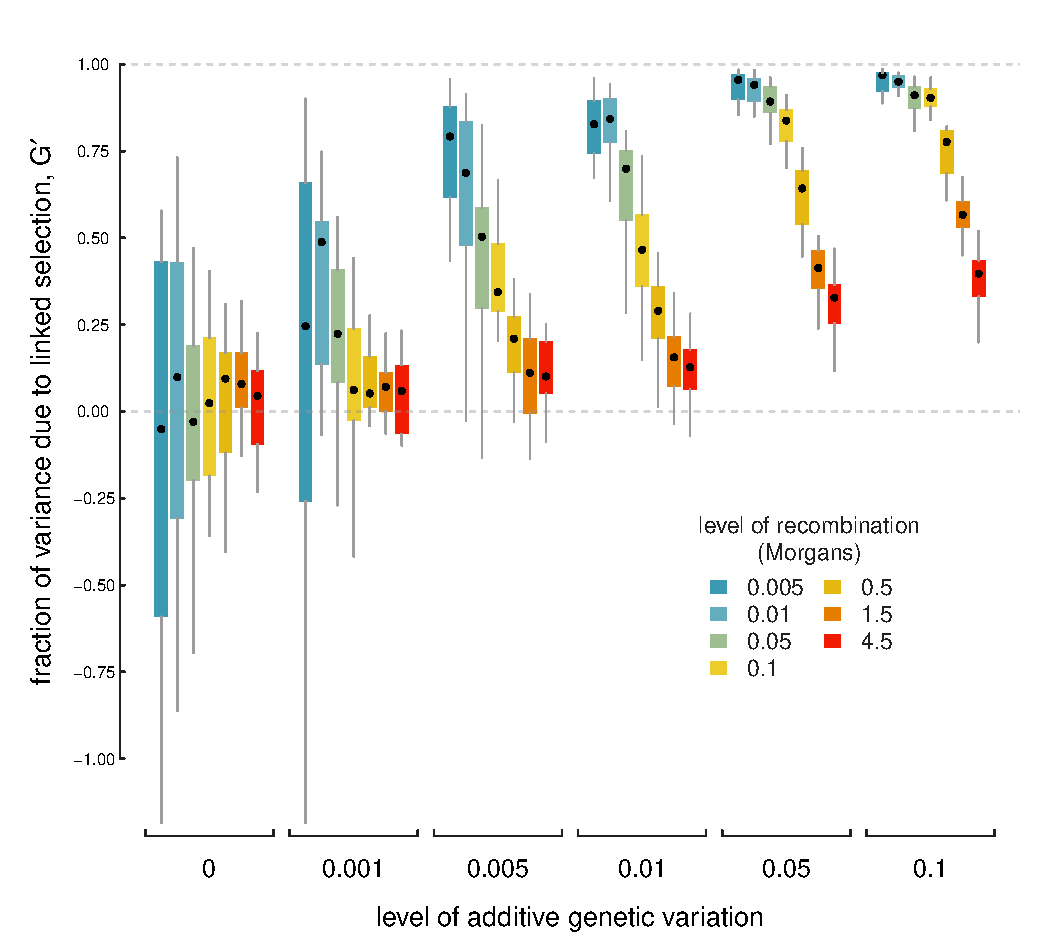
\includegraphics{./images/estimate-gp.pdf} 

  \caption{The proportion of total variance in allele frequency changes caused
    by linked selection, $G'$, across a variety of different levels of additive
    genetic variance (each group of boxplots), and different levels of
    recombination (each colored boxplot within a group). Each boxplot shows the
  spread of values across 20 replicates, with $\widehat{N}$ being calculated
across each replicate.} 

  \label{fig:est-g}
\end{figure}

First, a simple estimate of the total fraction of the variance in allele
frequency change ($G$) caused by linked selection is

\begin{align}
  \label{eq:g-def}
  G = \frac{\sum_{t \ne s}\cov(\Delta p_t, \Delta p_s)}{\var(p_t - p_0)}.
\end{align}

However, this estimator is conservative because it ignores the contribution
that linked selection has on the variance in allele frequency change across a
single generation (the $\var(\Delta_{_H} p_t)$ term in Equation
\ref{eq:var-decomp-1}). If we include these variance terms, we have a
less-conservative estimator we call $G'$,

\begin{align}
  G' &= \frac{\sum_{t \ne s}\cov(\Delta p_t, \Delta p_s) + \sum_{i=1}^t \var(\Delta_{_H} p_i)}{\var(p_t - p_0)} \nonumber \\
     &= 1 - \frac{\sum_{i=1}^t \var(\Delta_{_M} p_i) + \sum_{i=1}^t \var( \Delta_{_N} p_i)}{\var(p_t - p_0)}.
  \label{eq:g-prime}
\end{align}

We can think of the numerator of the second term in Equation \eqref{eq:g-prime}
as the variance in allele frequency change in a Wright--Fisher population
without selection.  Recall that under a Wright--Fisher model, the standardized
variance across $t$ generations is approximately $(1 - \exp(-\nicefrac{t}{2N}))
\approx p_0(1-p_0) \times \nicefrac{t}{2N}$, where this second approximation
works for short time spans ($\nicefrac{t}{2N} \ll 1$).  This suggests that we
can use our method-of-moments estimate of the effective population size without
the effects of selection, $\widehat{N}$, and compare the fraction of
standardized variance we expect under this rate of drift to the empirical
standardized variance,

\begin{align}
  G' &= 1 - \frac{t \E(p_{0}(1-p_{0})) }{2 \widehat{N} \var(p_{t} - p_{0}) }.
\end{align}

Figure \ref{fig:est-g} shows the estimated $G'$ from the method-of-moment
$\widehat{N}$ estimates using 20 replicates of simulated data. We learn
three important points about our $G'$ estimator. First, for low $V_A$, or $V_A
= 0$, the estimator is quite noisy. Second, although the signal can be noisy
for low $V_A$, the relationship between $G'$ and level of recombination is
consistent with selection affecting the total variance in allele frequency
changes across the genome. Finally, this suggests that a negative relationship
between $G'$ and recombination rate, calculated in windows across the genome,
is a robust signal of linked selection impacting the total variance in allele
frequency change. Furthermore, we would expect a positive relationship between
the number of coding basepairs per window (when such information is available)
and $G'$, which could serve as another robust signal of linked selection
impacting the total variance in allele frequency change.

\subsection{Fluctuating Selection}
\label{sec:fluct-sel}

Thus far we have assumed that fitness effect sizes are constant through time,
that is $\alpha_{t,l} =  \alpha_{s,l}$, for all $t, s$. In natural populations,
changes in the environment or composition of the population may cause these
effect sizes to change through time, due to changing selection pressures and
changes in the epistatic environment experienced by alleles. If these changes
occur within the timeframe of recorded allele frequency changes, the levels of
temporal autocovariance will differ from the levels predicted from our
directional selection theory. However, from Equation
\eqref{eq:multilocus-twopart} we can see that the magnitude of temporal
autocovariance is determined in large part by $\E(\alpha_t \alpha_s)$.

Here, we discuss how temporal autocovariance behaves under an example of strong
fluctuating selection: when selection on a trait changes direction at some
point. Specifically, we change the fitness function $w(z_i) = e^{z_i}$ to
$w(z_i) = e^{-z_i}$ after some timepoint $t^*$; this is equivalent to changing
$\alpha_{s,l} = - \alpha_{t,l}$ iff $s \ge t^*$, and $\alpha_{s,l} =
\alpha_{t,l}$ otherwise for all other $s < t^*$.

When such a strong change in the direction of selection occurs, the temporal
autocovariance between timepoints before and after the change becomes negative,
since temporal autocovariance is determined by the product $\alpha_{t}
\alpha_{s}$ for $t \ne s$ (here we are holding effects constant across loci).
We have validated this using the same simulation procedure as described in
Section \ref{sec:ml-sim}, except on generation 15 we reverse the direction of
selection on the trait by changing the fitness function $w(z) = e^z$ to $w(z) =
e^{-z}$. In Figure \ref{fig:fluct-sel}A, we show the temporal autocovariance
$\cov(\Delta p_5, \Delta p_s)$ for varying $s$ along the x-axis (in this case,
$V_a=0.05$, $R=0.1$, and $L=500$). During the first five generations, the
temporal autocovariance behaves as it does under directional selection,
decaying due to the decrease in additive genetic variance and the breakdown of
linkage disequilibrium. Then, on the $15^\text{th}$ generation, the direction
of selection on the trait with breeding value $z_i$ reverses and temporal
autocovariance becomes negative since $\alpha_{s,l} \alpha_{t,l} < 0$ for all
$s \ge t^*$ and $t < t^*$. Under this simple flip in the direction of selection
pressure, the genic variance, $V_a(s) = 2 \alpha^2 \sum_l p_{s,l}(1-p_{s,l})$,
in the expressions for the temporal autocovariance can be replaced with $V_a(s)
= 2 \alpha_s \alpha_t \sum_l p_{s,l}(1-p_{s,l})$, akin to a genetic/genic
covariance.  In Figure \ref{fig:fluct-sel}A, the gray line is our predicted
level of temporal autocovariance proportional to $V_A \mathcal{A}(R,t, s)$
given by Equation \eqref{eq:multilocus-cov-sum} before generation 15, and after
generation it is proportional to $-V_A \mathcal{A}(R,t, s)$ (using the
empirical additive genetic variance).  Note, however, that the dynamics of
additive genetic variance under fluctuating selection are more complex than
under directional selection.  Whereas under directional selection the genetic
variance decays as selection proceeds, under fluctuating selection there can be
a transient increase in the additive genetic variance (seen in Figure
\ref{fig:fluct-sel}A between generations 15-24).  This transient inflation
of the additive genetic variance is caused by the increase in the
heterozygosity of haplotypes that had experienced reduced heterozygosity due to
directional selection. With the direction of selection reversed, previously
selected haplotypes move to more intermediate frequencies, which increases the
additive genetic variance until selection proceeds and this variance decays
(generations 25 and onwards).  Overall, the dynamics of additive genetic
variance under fluctuating selection are more complicated than under
directional selection which makes inference using our sum of site
heterozygosity approximation infeasible.


\begin{figure}
  \centering
  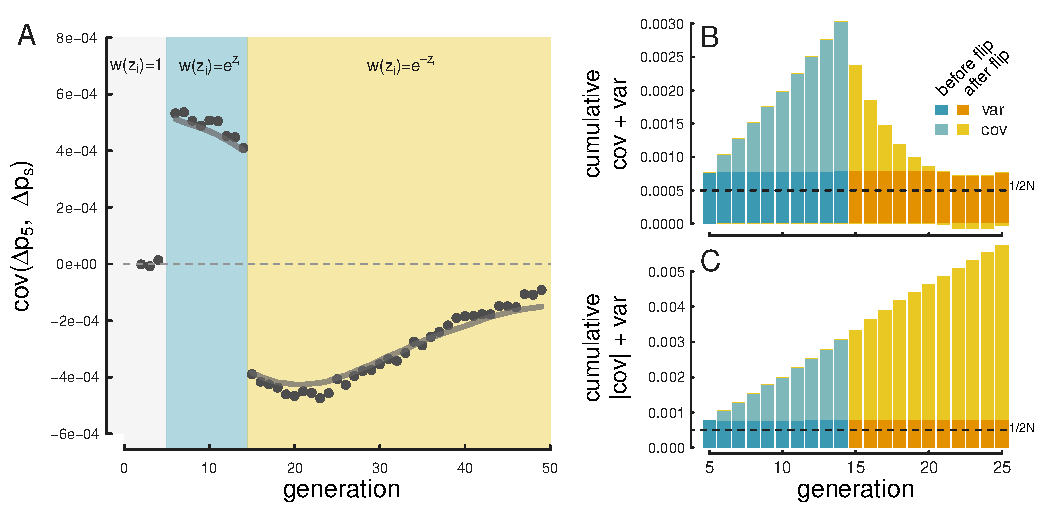
\includegraphics{./images/fluct-sel.pdf} 
  \caption{A: The covariance $\cov(\Delta p_5, \Delta p_s)$, where $s$
    is varied on the x-axis, for $V_a=0.05$, $R=0.1$, and $L=500$ averaged over
    100 replicates. Selection begins in generation 5 (with the fitness function
    $w(z_i)=e^{z_i}$) and on generation 15 the direction of selection flips (and
    the fitness function becomes $w(z_i) = e^{-z_i}$). The gray line shows our
    directional selection temporal autocovariance prediction modified so that
    after the flip in the direction the trait is selected, we plot the
    \emph{negative} theoretical level of temporal autocovariance. B:
    The average cumulative variance and covariances through the
    generations for the same simulation parameters, with the height of the bar
    representing the total cumulative variation $\var(p_t - p_0)/t$. Since the
    direction of selection flips, the covariances terms after generation 15
    become negative, leading the total variance to decrease (the negative
    covariances are plotted below the x-axis line). After generation 21, the
    total covariance is negative, leading the total variance to dip below the
    level of variance alone (determined by drift and heritable fitness
    variation). The dark gray dashed line shows the level of variance expected by
    drift alone ($\nicefrac{\var(p_t-p_0)}{t} = \nicefrac{1}{2N}$). C:
    The effect of using the absolute value of covariance, which prevents
    the negative autocovariances from canceling out the effects of other
    covariances before the direction of selection changed.} 
\label{fig:fluct-sel}
\end{figure}


Since fluctuating selection can create \emph{negative} temporal autocovariance,
the total amount of autocovariance over time (e.g. $\sum_{t\ne s} \cov(\Delta
p_t, \Delta p_s)$) can misrepresent the actual amount that linked selection is
affecting allele frequencies on shorter timescales. This, in turn, leads our
estimator $G$, for the fraction of variance in allele frequency due to linked
selection, to underestimate the total contribution of linked selection to
variation in allele frequencies over the time period.  We show an example of
this in Figure \ref{fig:fluct-sel}B, which depicts the total variance in
allele frequency change $\nicefrac{\var(p_t - p_0)}{t}$ through time,
partitioned into variance and covariance components and colored according to
whether the generation was before and after the reverse in directional
selection. The covariances $\sum_{t\ne s} \cov(\Delta p_t, \Delta p_s)$
increase as they would under directional selection, but after generation 15,
the contribution of covariance begins to decrease as negative autocovariances
accumulate. By generation 20, the total covariance terms have a net negative
effect, and actually act to decrease the total variance $\nicefrac{\var(p_t -
p_0)}{t}$ for a few generations below the constant level expected under drift
and heritable variation.

To more fully capture the contribution of selection allele frequency change, we
modify $G$, using the absolute value of the covariances, 

\begin{align}
  \label{eq:g-abs}
  G_{abs} = \frac{\sum_{t \ne s}|\cov(\Delta p_t, \Delta p_s)|}{\var(p_t - p_0)}
\end{align}
%

which prevents negative temporal autocovariances from canceling out the effects
of positive temporal autocovariances, since both are a reflection of linked
selection acting on neutral allele frequency changes. We show $G_{abs}$ in
Figure \ref{fig:fluct-sel}C, where even after the change in the directional
selection we see a steady accumulation of covariance contributing to total
variance $\nicefrac{\var(p_t - p_0)}{t}$. This also suggests one plausible way
to check for genomically wide-spread fluctuating selection would be to test if
$G_{abs} > G$. However, we note that in contrast to our simulations, it is
likely that in natural populations only a subset of alleles change their
relationship to fitness. This may act to dampen the magnitude of, but not
completely reverse the direction of genome-wide temporal autocovariance, and so
different approaches may be needed to identify fluctuations.

\section{Discussion}

Currently, the prevailing empirical approach to studying linked selection
relies on using samples from a single timepoint and modeling the patterns of
diversity subject to different functional constraints and in different
recombination environments. The early theoretical work underpinning empirical
analyses of linked selection's effects on diversity were primarily full sweep,
recurrent hitchhiking models, where beneficial mutations arise in the
population and then sweep to fixation
\parencite{Maynard_Smith1974-lc,Stephan1992-jc,Kaplan1989-ld}. Furthermore, by
looking at the patterns of diversity around amino acid substitutions or the
site frequency spectrum in low recombination regions, researchers have teased
apart the effects of background selection and hitchhiking in \emph{Drosophila}
\parencite{Begun2007-bg,Elyashiv2016-vt}, humans
\parencite{Hernandez2011-gs,McVicker2009-ax}, and some plants species
\parencite{Nordborg2005-vt,Beissinger2016-cm,Schmid2005-on,Williamson2014-oy}.
Yet, as other theoretical models of hitchhiking incorporating changes in the
environment \parencite{Kopp2007-mc,Kopp2009-lo,Kopp2009-pj}, sweeps originating
from standing variation \parencite{Hermisson2005-hs}, and multiple competing
beneficial haplotypes \parencite{Pennings2006-lj} have been developed, it has
become rather more difficult to detect the signal of these hitchhiking
phenomenon in empirical data. We have proposed here that temporal autocovariance
offers a unique and measurable signal of linked selection over shorter
timescales that provides a fuller picture of the ways in which genome-wide
diversity has affected by these other hitchhiking phenomena. 

\subsection{Empirical Applications and Future Directions}

Here, we've developed expressions for temporal variances and autocovariances,
and applied these to model temporal variances and covariances during
directional selection on a trait. We have demonstrated how one can (1) estimate
the additive genetic variance for fitness and the drift-effective population
size, (2) estimate the fraction of variance in allele frequency change due to
linked selection, and (3) evaluate whether fluctuating selection is operating
from these temporal variances and autocovariances. However we recognize a
series of limitations and difficulties when applying these methods to empirical
data and natural populations.

First, one difficulty with temporal sampling of natural populations is the risk
that the genetic composition may change drastically due to migration or biased
sampling across timepoints. Since our theory assumes a constant-sized and
isolated population, migration into the sampled population presents a serious
potential confounder. For example, seasonal migration could create an influx of
new alleles that could at best dampen signals of directional selection across
seasons, or at worst create a signal of artificial covariance between like
seasons. Similar biases could occur if a sampling method incidentally preferred
certain subgroups in a stratified population. This could occur, for example, if
individuals differ in some behavior affecting their likelihood of being sampled
across different temporal environments, which could cause spurious covariances.
While such sampling issues and migration might be able to be detected
\emph{post hoc} from exploratory data analysis approaches like PCA, studying
isolated natural populations and carefully designing sampling schemes would
lead to the best inference. Importantly, the effects of gene flow and other
temporal inhomogeneities could differ across recombination environments, as
among population differentiation will be more pronounced in regions of low
recombination and high functional density
\parencite{Keinan2010-ry,Burri2017-ml,Nachman2012-sw}. In situations where
  migration is a factor, one way forward might be to study the contribution of
  linked selection after partitioning out the effects of gene flow across
  recombinational and functional environments by extending admixture inference
approaches that estimate the genome-wide effect of drift and admixture.

Second, our method-of-moments approach relies on assuming we can approximate
the dynamics of \vb{the decay of the additive genetic variance that was present
at a reference timepoint} by using the observed changes in sum of site
heterozygosity in a region as a proxy for its decay. While we have shown this
model works under directional selection in a relatively idealized setting,
inference in natural populations may be complicated by changes in the
environment that induce the effect sizes across loci to vary across timepoints.
While our fluctuating selection results show that our directional selection
theory extends to changes in the direction of selection with minor adjustments
(e.g. Figure \ref{fig:fluct-sel}), having the effect sizes vary across each
generation would complicate the dynamics of additive genetic variance through
time and make inference of $V_A$ difficult.  Similarly, we assume that effect
sizes are constant across sites. Variance in effect sizes across a region will
not bias our results unless there is covariance between effect size and local
recombination rate. Further work is required to develop statistical methods to
test for violations of our assumptions about effect sizes remaining constant
across time, and to potentially incorporate these complications into inference.

Along similar lines, we have focused on directional selection under a
multiplicative model. However, selection experiments, a natural place to apply
our method, often use truncation selection, which generates systematic
epistasis for fitness and thus linkage disequilibria among loci
\parencite{Burger2000-an,Walsh2018-bt}. Similarly, in natural populations
stabilizing selection will act on many traits, which can also generate LD among
loci. These selective processes will act to rapidly reduce the additive genetic
variance for fitness across time, especially in low recombination regions, and
to reduce the initial additive genetic variance in low recombination regions.
Simulating the effect of truncation selection and stabilizing selection on
temporal covariances in allele frequencies seems a useful direction. Our model
may prove to be a useful null model of selection that the complications of
epistasis \vb{and different dynamics of the additive genetic variance} could be
tested against. 

Finally, while we demonstrate that our method-of-moments estimation approach is
simple and leads to unbiased estimators, we see opportunities for simple
extensions and other inference procedures. Differences in recombination rates
and coding density are relatively easily accommodated (Equation
\ref{eq:mom-windows-cbp}). In fitting our model we assumed a parametric form to
the initial LD between neutral and selected loci; however, in practice the
initial linkage disequilibria between neutral polymorphisms and putatively
functional sites could be estimated empirically. Using the empirical LDs in
Equation \eqref{eq:mom-windows-cbp} could make the inference somewhat analogous
to LD Score regression \parencite{Bulik-Sullivan2015-ls}. The LD Score of a SNP
is simply the sum of the $R^2$'s of the focal SNP to all SNPs within some large
physical genomic window, which could be used in place of the integral in
Equation \eqref{eq:multilocus-triangle}. Using this equation, $V_A$ could be
estimated by regressing the temporal covariance of a SNP on its LD Score. An
alternate approach would be to use likelihood methods to model each neutral
site's frequency changes using the set of pairwise linkage disequilibria and
recombination distances between the neutral site and all neighboring
polymorphic sites. Then, genome-wide or region-wide estimates could be found
via composite likelihood methods, in a similar manner to
\textcite{McVicker2009-ax} and \textcite{Elyashiv2016-vt}. Furthermore, one
could include different $V_A$ parameters for neighboring polymorphic sites with
specific functional annotations, such as those in genic regions, introns,
exons, etc. to see how different classes of sites contribute to the additive
genetic variance for fitness. Our hope is that statistical methods to quantify
the effects of linked selection over short timescales will improve and be
combined with measures of phenotypic change, leading to a more synthetic view
of how selection on ecological timescales occurs at the genetic and phenotypic
levels.

As the number of empirical temporal genomic studies continue to increase, it is
worth mentioning how our study of temporal autocovariance suggests a few ways
to optimize experimental design to increase the power to differentiate the
effects of selection from drift. First, one should ideally sample frequencies
from consecutive generations for at least some timepoints during the duration
of the experiment. This is because the variance in allele frequency change
$\var(\Delta p_t)$ between adjacent generations is only impacted by the
heritable variance in offspring number, $\var(\Delta_{_H} p_t)$ (see Equation
\ref{eq:var-decomp-1}), and not by the accumulation of temporal autocovariance
terms (e.g. Equation \ref{eq:var-decomp}); this allows for more accurate
estimates of $G$. In cases where a long study duration is needed but sequencing
is limited to only a subset of generations, a mixed duration sampling design,
such as sampling generations 1 through 4, and then 10 through 14, and so forth
could serve as a compromise. Second, as described in Appendix Section
\ref{sec:sampling}, the shared sampling noise between adjacent timepoints
creates a negative bias in autocovariance that must be corrected for. As
described in Equations \eqref{eq:corrected-var} and \eqref{eq:corrected-cov},
we can estimate this bias from data, but this introduces additional uncertainty
into our parameter estimates. In cases where the experimenter suspects \emph{a
priori} that fluctuating selection is occurring, e.g. between two seasons, we
recommend at least two temporal samples per season. This allows one to
differentiate negative covariance occurring from the bias correction procedure
underestimating bias from negative covariance caused by fluctuating selection
through comparing non-adjacent timepoints that differ in season. Finally, once
can directly remove the effects of the technical sampling noise created by
variation in sequencing by dividing up temporal samples and barcoding them into
two groups (e.g. A and B). Then, the sample covariance estimate $\cov(\Delta
p_{t,A}, p_{s,B})$ does not share the technical sampling noise, reducing the
bias (but note some bias remains due to the sampling process where individuals
are sampled from the population.)

\subsection{Connecting Temporal Linked Selection with Single Timepoint Studies}

Our goal in this paper is to suggest that quantifying variance and
autocovariance using temporal data sets can help us understand the impact
linked selection has across the genome on short timescales, which supplements
our current view informed mainly by single timepoint studies. A range of
approaches to estimate the parameters and impact of models of linked selection
from a single contemporary timepoint have been developed
\parencite{Wiehe1993-ja,Begun1992-ey,Sella2009-rf,Elyashiv2016-vt,McVicker2009-ax,Hudson1994-yq}.
These estimates necessarily reflect linked selection over tens to hundreds of
thousands of generations. One question is whether these estimates of the
proportion of allele frequency change due to linked selection should line up
with those over shorter time periods? Some forms of linked selection may be
fairly uniform over time, whereas rare, strong sweeps will have a huge impact
on long-term patterns of variation but may be hard to catch in temporal data.
Conversely, as we discuss below, fluctuating selection may lead to stronger
signals of linked selection on short timescales than seen in long-term
snapshots.

Studies of contemporary data have revealed multiple lines of evidence for the
effect of linked selection in a variety of taxa. If linked selection is
pervasive across the genome, diversity could be severely dampened as most sites
would be in the vicinity of selected sites, thus reducing the genome-wide level
of diversity without leaving strong local signals differentiated from the
background. This is one proposed resolution of Lewontin's paradox, the
observation that diversity levels occupy a narrow range across taxa with
population sizes that vary by orders of magnitude
\parencite{Lewontin1974-jb,Maynard_Smith1974-lc,Gillespie2001-ll,Leffler2012-zj}.
\textcite{Elyashiv2016-vt} estimated a $77$ - $89\%$ reduction in neutral
diversity due to selection on linked sites in \emph{Drosophila melanogaster},
and concluded that no genomic window was entirely free of the effect of
selection. Similarly, \textcite{Corbett-Detig2015-gt} has found evidence of a
stronger relative reduction in polymorphism due to linked selection in taxa
with larger population sizes. However, these reductions fall short of the many
orders of magnitude required for linked selection to explain Lewontin's paradox
\parencite{Coop2016-gx}.   

One limitation of these approaches is that they require estimating $\pi_0$, the
level of diversity in the absence of linked selection, usually from the
diversity in high-recombination regions with low gene content. The average
genome-wide reduction of diversity can then be judged relative to $\pi_0$.
Ideally, $\pi_0$ would be a measure of the average diversity due entirely to
drift and demographic history, i.e. unaffected by heritable fitness variation.
However, there are two complications with this. First, as
\textcite{Robertson1961-ho} first showed, even a site completely unlinked from
sites creating heritable fitness variation experiences a reduced effective
population size due to the total additive genetic variance for fitness at these
unlinked sites, and thus lower diversity (see also \cite{Santiago1995-hx}). The
second complication is that if linked selection is sufficiently strong, the
bases used to measure $\pi_0$ may not be sufficiently unlinked from
fitness-determining sites to plateau to the \textcite{Robertson1961-ho} level
of diversity, a known potential limitation
\parencite{Coop2016-gx,Elyashiv2016-vt}. Overall, the empirical studies relying
on present-day samples from a single timepoint could be underestimating the
effects pervasive linked selection has on diversity. If linked selection can be
observed over suitable timescales in temporal data, we might be able to
disentangle some of these effects. For example, if high recombination regions
still show temporal autocovariance in allele frequency change, we would have
evidence that even these regions are not free of the effect of linked selection
and we might be able to estimate its long term impact on levels of diversity. 

Temporally or spatially fluctuating selection has long been discussed as an
explanation for abundant, rapid phenotypic adaptation over short timescales,
yet over longer timescales both phenotypic changes and molecular evolution
between taxa are slow \parencite{Messer2016-mn,Hendry1999-zu,Gingerich1983-cc}.
However, most of our approaches to population genomic data are built on simple
models with constant selection pressures, as typically we have not had the data
to move beyond these models \parencite{Messer2016-mn}. Currently, many
approaches to quantify the impact of linked selection due to hitchhiking assume
classic sweeps, where a consistent selection pressure ends in the fixation of a
beneficial allele \parencite{Sella2009-rf,Hernandez2011-gs,Wiehe1993-ja}.
However, fluctuating selection can have a larger effect on reducing diversity
than classic sweeps \parencite{Barton2000-zg} depending on the timescales over
which such fluctuations occur. In fact as \textcite{Barton2000-zg} points out,
the total effect of classic Maynard-Smith and Haigh-type sweeps on diversity is
limited by the relatively slow rate of substitutions. We show that when the
direction of selection on a trait abruptly reverses, this creates negative
autocovariance between the allele frequency changes before and after the
reverse in direction. We can observe the shift by plotting autocovariances over
time and noting when they become negative, indicating a negative additive
genetic covariance between fitness at two timepoints. Here we assume a simple
form of fluctuating selection: where selection pressures on all of our sites
flip at some timepoint. In reality, selection pressures will change on only
some traits, and some of the genetic response will be constrained by
pleiotropy, thus only some proportion of the additive genetic variance will
change. Still, we expect some level of negative covariance after a reversal in
the direction of selection, and there is additional signal of fluctuating
selection by comparing how the strength of temporal autocovariance varies with
recombination and the initial level of linkage disequilibrium in the genome.

\subsection{Connecting Estimates of $V_A$ from Temporal Genomic Data and
Quantitative Genetic Studies}

The temporal covariance of allele frequencies potentially offers a way to
estimate the additive genetic variance for fitness, as illustrated by our
method-of-moments approach across genomic windows. The additive genetic
variance for fitness can, like any other trait, be estimated through
quantitative genetics methods, which exploit the phenotypic resemblance between
relatives and their known kinship coefficients
(\cite{Kruuk2004-zk,Shaw2013-rx}; see \cite{Hendry2018-se} for a review), and
these methods have been applied to estimate the additive genetic variance for
fitness from natural populations \parencite{Burt1995-dd,Mousseau1987-uy,}.
Ideally, one could reconcile quantitative genetic measures of fitness variance
with estimates from allele frequency covariance. For example,
\textcite{Charlesworth2015-am} undertook a similar analysis in \emph{Drosophila
melanogaster}, comparing population genetic estimates of fitness variance to
quantitative genetics estimates, highlighting a discordance potentially
consistent with undetected large-effect alleles that are likely maintained by
some form of balancing selection. By allowing us to directly measure fitness
variation from population genetic data over very short timescales, temporal
data could help untangle the causes of this discordance. A natural extension of
this would be to see which regions contain the greatest inferred levels of
additive genetic variance for fitness, and test for functional covariates such
as the number of coding bases, etc. Whereas previous temporal studies have
focused on finding loci under selection, inferring the level of additive
genetic variance could provide a more complete view of how much selection
operates over short timescales.

\subsection{Concluding Thoughts}

With temporal data we can directly partition the total variance in allele
frequency change across generations, $\var(p_t-p_0)$ into components according
to the underlying process governing their dynamics: drift and linked selection.
Since the trajectory of a neutrally drifting polymorphism does not autocovary,
evidence of temporal autocovariance across neutral sites in a closed population
is consistent with linked selection perturbing these sites' trajectories. If we
consider drift to be the process by which non-heritable variation in
reproductive success and Mendelian segregation cause allele frequencies to
change, then this is estimable from and separable from the effects of linked
selection using temporal data. This helps frame the long-running debate about
the roles neutral drift and linked selection have in allele frequency dynamics
into a problem that can potentially be directly quantified by the contribution
of each distinct process with temporal data.

\section{Code and Data Availability}

All code and simulation data to reproduce these results are available on GitHub
at \url{https://github.com/vsbuffalo/tempautocov}.

\section{Acknowledgments}

We thank Nick Barton, Doc Edge, Matt Osmond, Enrique Santiago, Michael Turelli,
and two anonymous reviewers for feedback on previous versions of the
manuscript, and Aneil Agrawal, Dave Begun, Sarah Friedman, Bill Hill, John
Kelly, Tyler Kent, Chuck Langley, Sally Otto, Jonathan Pritchard, Kevin
Thornton, Anita To, and members of the Coop lab for helpful conversations.
This research was supported by an NSF Graduate Research Fellowship grant
awarded to VB (1650042), and NIH (R01-GM108779) and NSF (1353380) awarded to
GC.

%\bibliographystyle{chicago}
\printbibliography


\newpage


\appendix

\section{Appendix} 
\counterwithin{figure}{section}
\setcounter{figure}{0}    

\begin{table}[!htbp]
  \caption{Notation}
  \begin{tabular}{r|p{12cm}}
 Symbol & Usage  \\ \hline
 $p_t$ & Allele frequency in generation/timepoint $t$  \\
 $\Delta p_t$ & Allele frequency change between generations $t+1$ and $t$, $\Delta p_t = p_{t+1} - p_t$ \\
 $\Delta_{_N} p_t $ & Frequency change due to non-heritable variation in fitness, \eqref{eq:delp-decomp}, \eqref{eq:var-decomp-1}  \\
 $\Delta_{_M} p_t $ & Frequency change due to Mendelian segregation, \eqref{eq:delp-decomp}, \eqref{eq:var-decomp-1} \\
 $\Delta_{_H} p_t $ & Frequency change due to heritable differences, \eqref{eq:delp-decomp}, \eqref{eq:var-decomp-1} \\
 $N$ & Census population size of breeding individuals \\
 $N_e$ & Effect population size \\
 $f_i$ & Fitness (expected number of offspring) of individual $i$, \eqref{eq:ap-freq}\\
 $\alpha_{t,l}$ & Effect size in generation $t$ and locus $l$, \eqref{eq:neut-change}, \eqref{eq:ap-delta-H} \\
 $L$ & Total number of loci impacting fitness, \eqref{eq:neut-change} \\
 $g_{i,l} \in \{0, 1, 2\}$ & Individual $i$'s gene count at locus $l$, \eqref{eq:ap-delta-H-2} \\
 $x_{i} \in \{0, 1, 2\}$ & Individual $i$'s neutral gene count at the tracked neutral site, \eqref{eq:neut-change}, \eqref{eq:ap-delta-H-2}, \eqref{eq:ap-delta-H-3} \\
 $D_{t,l}$ or $D_{t,l}'$ & \hangindent=1em Gametic linkage disequilibrium between the tracked neutral site and selected locus $l$ at time $t$, Supplementary Figure \ref{fig:ld-cartoon}, \eqref{eq:neut-change}, \eqref{eq:ap-delta-H-2}, \eqref{eq:ap-delta-H-3} \\
 $D_{t,l}''$ & \hangindent=1em Non-gametic disequilibrium between the tracked neutral site and selected locus $l$ at time $t$, Supplementary Figure \ref{fig:ld-cartoon}, \eqref{eq:neut-change}, \eqref{eq:ap-delta-H-2}, \eqref{eq:ap-delta-H-3} \\
 $\E(\mathcal{R}_{t,l}^2)$ & \hangindent=1em The squared correlation coefficient of linkage disequilibrium between the tracked neutral site and selected site $l$ at time $t$, \eqref{eq:cov-R}, \eqref{eq:ap-D}\\
 $r_l$ & \hangindent=1em The recombination fraction between the tracked neutral site and selected site $l$\\
 $V_a(s)$ & The additive genic variance, \eqref{eq:multilocus-cov-sum} \\ 
 $V_A(s)$ & The additive genetic variance, \eqref{eq:var-genic-z} \\ 
 $R$ & The total level of recombination in the region, in Morgans, \eqref{eq:ave-neut-autocov} and Figure \ref{fig:cartoon} \\ 
 $r(g)$ & \hangindent=1em A mapping function (i.e. Haldane's), which maps a position $g$ to a recombination fraction.\\ 
 $\rho$ & The population recombination rate, $\rho = 4Nr$, Section \ref{sec:temp-autocov-aveneut} \\ 
 $\mathcal{A}(R, t, s)$ & \hangindent=1em The average linkage disequilibrium in a region of $R$ Morgans, that persisted from generation $t$ to generation $s$, \eqref{eq:multilocus-triangle} \\
 $V_N$ & The non-heritable variance in offspring number, \eqref{eq:multilocus-var} \\
 $SSH(t)$ & The sum of site heterozygosity at selected sites time $t$, \eqref{eq:VA-SSH} \\
 $SSH_n(t)$ & The sum of site heterozygosity at neutral sites at time $t$, \eqref{eq:VA-SSH} \\
 $ssh_n(t)$ & \hangindent=1em The proportion of sum of site heterozygosity at neutral sites at time $t$ relative to $SSH(1)$, $SSH_n(t) / SSH_n(1)$ \eqref{eq:VA-ssh} \\
 $z_i$ & \hangindent=1em The breeding value of the trait that determines fitness, $z_i = \sum_{i=1}^L \alpha g_{i,l}$, see appendix section \ref{ap:multilocus} \\
 $w(z_i)$ & The fitness of individual $i$ with fitness function $w(\cdot)$, see appendix section \ref{ap:multilocus} \\
\end{tabular}
\end{table}

\begin{table}[!htbp]
  \setcounter{table}{0}
  \caption{Notation, continued}
  \begin{tabular}{r|p{12cm}}
 Symbol & Usage  \\ \hline
 $\mathbf{Q}$ & The sample standardized variance-covariance matrix, \eqref{eq:ave-temp-autocov} \\
 $Q_{t,s}$ & The elements of the observed sample matrix $\mathbf{Q}$, \eqref{eq:ave-temp-autocov} \\
 $\mathbf{\Sigma}$ & \hangindent=1em The standardized variance-covariance matrix, based on our theoretical expressions \\
 $\Sigma_{t,s}$ & The elements of the standardized variance-covariance matrix, \eqref{eq:multilocus-triangle}, \eqref{eq:multilocus-var} \\
 $\Delta p_{n,t}$ & \hangindent=1em The allele frequency change at site $n$ between times time $t+1$ and $t$, \eqref{eq:ave-temp-autocov} \\
 $\tau$ & \hangindent=1em The number of allele frequency changes observed, e.g. after sampling for $\tau + 1$ timepoints \\
 $V_{a,ssh_n}(t)$ & \hangindent=1em The additive genic variation at time $s$ as approximated by the observed decay in the sum of site heterozygosity at neutral sites, \eqref{eq:VA-ssh} \\
 $\var_i(z_i)$ & The variance in trait values taken over individuals, \eqref{eq:var-genic-z} \\
 $\widehat{V_A(1)}$ & \hangindent=1em The method-of-moments estimate of the additive genetic variance in the first generation, \eqref{eq:mom-moments-cov}, \eqref{eq:mom-moments-var} \\
 $\widehat{F}$ & \hangindent=1em The method-of-moments estimate of Wright's standardized variance, $F = \nicefrac{1}{2N}$, \eqref{eq:mom-moments-cov}, \eqref{eq:mom-moments-var} \\
 $\widehat{N}$ & \hangindent=1em The method-of-moments estimate of drift-effective population size, $N = \nicefrac{1}{2F}$ \\
 $\sigma^2$ & \hangindent=1em The sampling noise around each element of the sample variance-covariance matrix. \\
 %$\vec{a}, \; \vec{b}$ & Vectors of the 
 $B$ & The total number of windows after partitioning the genome, \eqref{eq:mom-windows} \\
 $w_{text{BP}}$ & Width of windows (in basepairs), \eqref{eq:mom-windows} \\
 $v_A(1)$ & The average additive genetic variance per basepair \\
 $w_{\text{CBP}}$ & Number of coding basepairs in a window, \eqref{eq:mom-windows} \\
 $W_{\text{CBP}}$ & Total number of coding basepairs in the genome, \eqref{eq:mom-windows-cbp}  \\
   $G$ & \hangindent=1em A conservative measure of the total variance in allele frequency change due to linked selection, \eqref{eq:g-def} \\
   $G'$ & \hangindent=1em An alterate, less conservative measure of the total variance in allele frequnecy change due to linked selection, \eqref{eq:g-prime} \\
   $G_{abs}$ & A variant of $G$ using the absolute value of covariances, \eqref{eq:g-abs} \\
\end{tabular}
\end{table}

\subsection{Decomposition of Allele Frequency Change}
\label{ap:decomp}

This decomposition of \emph{neutral} allele frequency change between two
consecutive generations is based on that of \textcite{Santiago1995-hx}. We
imagine a closed Wright--Fisher population of $N$ diploids, where each diploid
$i$ contributes $k_i \sim \text{Multinom}(\nicefrac{f_i}{N}, 2N)$ gametes to
the next generation. We assume that the population size is constant, such that one
diploid begets one diploid and thus $\E_i(f_i) = 1$. The neutral allele
frequency in the next generation can be thought of as each of the $N$ parents
passing their average genotype $\nicefrac{x_i}{2}$ (where $x_i \in\{0, 1, 2\}$
is the number of tracked neutral alleles individual $i$ carries) to their $k_i$
gametes, plus a random Mendelian deviation $b_{ij} \in \{0, -\nicefrac{1}{2},
\nicefrac{1}{2}\}$ to each offspring $j$. Then, the frequency in the next
generation can be written as

\begin{align}
  p_1 &= \frac{1}{N} \sum_{i=1}^N \left(k_i \frac{x_i}{2} + \sum_{j=1}^{k_i} b_{ij} \right)
  \label{eq:ap-freq}
\end{align}
%
where $b_{ij} = \delta_{x_i, 1} (\nicefrac{1}{2} - B_j)$, $B_j \sim
\text{Bernoulli}(\nicefrac{1}{2})$ and $\delta_{x_i, 1}$ is an indicator
function that is one when the individual $i$ is a heterozygote (i.e. $x_i=1$),
and zero otherwise.

If we further decompose the number of offspring of individual $i$ into the
genetic and non-genetic contributions, $k_i = f_i + d_i$, then

\begin{align}
  p_1 &= \frac{1}{N} \sum_{i=1}^N \left( (f_i + d_i) \frac{x_i}{2} + \sum_{j=1}^{k_i} b_{ij} \right) \nonumber \\
      &= \frac{1}{2N} \sum_{i=1}^N f_i x_i + \frac{1}{2N} \sum_{i=1}^N d_i x_i + \frac{1}{N} \sum_{i=1}^N  \sum_{j=1}^{k_i} b_{ij} 
\end{align}
%
and the change of the neutral allele's frequency is the difference $\Delta p = p_1 - p_0$ where $p_0 = \nicefrac{1}{2N} \sum_{i=1}^{N} x_i$. Then,

\begin{align}
\Delta p = p_1 - p_0 &= \frac{1}{2N} \sum_{i=1}^N f_i x_i + \frac{1}{2N} \sum_{i=1}^N d_i x_i + \frac{1}{N} \sum_{i=1}^N  \sum_{j=1}^{k_i} b_{ij} - \frac{1}{2N} \sum_{i=1}^N x_i \nonumber \\
                     &= \underbrace{\frac{1}{2N}\sum_{i=1}^N x_i (f_i - 1)}_{\Delta_{_H} p_1} + \underbrace{\frac{1}{2N} \sum_{i=1}^N d_i x_i}_{\Delta_{_N} p_1} + \underbrace{\frac{1}{N} \sum_{i=1}^N \sum_{j=1}^{k_i} b_{ij}}_{\Delta_{_M} p_1}.
\end{align}
%

These $d$'s broadly capture non-heritable variation in an individual's
offspring number, with $\E[d_i]=0$. In a quantitative genetics framework
$\var_i(d_i)$ can include non-genetic variation in the lifetime reproductive
success of individuals ($V_E$), in population genetic models $\var_i(d_i)$ can
accommodate the sampling of parents to form the next generation, e.g.
multinomial sampling of individuals from fitnesses \parencite{Santiago1995-hx}.
From now forwards, we assume that variation in these $d$'s is non-heritable. We
note that in non-panmictic populations, chance covariances could be created
between a neutral polymorphism and environmental component of their phenotype,
especially as a population expands its range into new environments that affect
the phenotype, and variants ``surf'' to higher frequencies
\parencite{Edmonds2004-xf,Hallatschek2008-mn,Excoffier2008-ep}.

Note that by construction, the allele frequency change components $\Delta_{_N}
p_t$ $\Delta_{_M} p_t$, and $\Delta_{_H} p_t$ are orthogonal within each
individual, given the neutral allele frequency $x$. Partitioning the allele
frequency change for an individual $i$ into its components,

\begin{align}
  \Delta p_{t,i} &= \underbrace{\frac{1}{2} x_i (f_i - 1)}_{\Delta_{_H} p_{t,i}} + 
       \underbrace{\frac{1}{2} x_i d_i}_{\Delta_{_N} p_{t,i}} + 
       \underbrace{\delta_{x_i,1}(\nicefrac{k_i}{2} - M(k_i))}_{\Delta_{_M} p_{t,i}} \\
       &= \frac{1}{2} x_i (f_i - 1) + 
       \frac{1}{2} x_i d_i + 
       \delta_{x_i,1}(\nicefrac{f_i}{2} - M(f_i)) + 
       \delta_{x_i,1}(\nicefrac{d_i}{2} - M(d_i))
\end{align}
%
where $M(n) = \sum_{j=1}^{n} B_j \sim \text{Binom}(n, \nicefrac{1}{2})$.

Two random variables $X, Y$ are uncorrelated if $\cov(X, Y) = \E(XY)
- \E(X)\E(Y)= 0$, and are orthogonal if either has an expected value of zero
such that $\E(XY) = 0$. We show briefly that taking expectations \emph{over
conceptual evolutionary replicates}, the terms are orthogonal. First, the terms
$x(f-1)$ and $x d$ are orthogonal (dropping $i$ subscripts),

\begin{align}
  \nicefrac{1}{4} \cov(x(f-1), x d) &= \nicefrac{1}{4}(\E(x^2 d (f-1)) - \E(x(f-1)) \E(x d)) \nonumber \\
                                    &= \nicefrac{1}{4} (\E(x^2) \E(d) \E(f-1) - \E(x)\E(f-1) \E(x d)) \nonumber \\
                                    &= 0
\end{align}
%
since $\E(f) = 1$ across evolutionary replicates due to the assumption that
population size is constant, and $x \perp f$, as across all evolutionary
replicates, there is no dependence between a particular neutral allele an
individual carries and their fitness (though in particular replicates, such
associations occur). Similarly, for the case $x=1$ (other cases are all zero,
and can be ignored), it can be shown using the law of total expectation that
$\cov(x d, \nicefrac{d}{2} - M(d)) = 0$ (and likewise with $x (f-1)$ and
$\nicefrac{f}{2} - M(f)$). Note that across individuals within a population,
there are weak covariances in their number of offspring as the total number of
offspring must sum to $N$; under a Multinomial offspring distribution, these
are of order $\nicefrac{1}{N}$.


\subsection{Temporal variance and autocovariance under multilocus selection}
\label{ap:multilocus}

We assume the phenotype of an individual $i$ has an additive polygenic basis,
such that their breeding value is $z_i = \sum_{l=1}^L \alpha_{t,l} g_{i,l}$
which deviates around a mean of zero, and $\alpha_{t,l}$ is the additive effect
size at locus $l$ in generation $t$, and $g_{i,l} \in \{0,1,2\}$ is individual
$i$'s allele count at this locus (note that effect of non-heritable
environmental noise affecting the trait is accounted for in the $d_i$ terms
above). We impose directional selection on this trait using an exponential
fitness function, such that individual $i$'s fitness is $f_i =
\nicefrac{w(z_i)}{\bar{w}} \approx e^{z_i}$ (assuming $\bar{w} \approx 1$). If
we assume individuals' phenotypic values do not deviate too far from their mean
value of zero, we can approximate $f_i$ as: $f_i \approx 1 + \sum_{l=1}^L
\alpha_{t,l} g_{i,l}$. Then, we can write the change in neutral allele
frequency due to only heritable variation in fitness ($\Delta_{_H} p_t$) as a
covariance between fitness and the neutral allele frequency across individuals
in generation $t$, 

\begin{align}
  \Delta_{_H} p_t &= \frac{1}{2N} \sum_{i=1}^N x_i \left(f_i - 1\right) \\
                  &= \frac{1}{2} \cov_i(x_i, f_i) \\
                  &= \frac{1}{2} \cov_i(x_i, \sum_{l=1}^L \alpha_{t,l} g_{i,l})
  \label{eq:ap-delta-H}
\end{align}
%
which is the is the Robertson-Price covariance
\parencite{Price1970-si,Robertson1966-fs,Lynch1998-wl,Walsh2018-bt}.

Now, we break up the genotypic value $x_i$ into the contributions of each of
the two gametes that formed individual $i$, $x_i = x_i' + x_i''$, and likewise
with the trait locus $g_{i,l} = g_{i,l}' + g_{i,l}''$, where $x_i', x_i'',
g_i',$ and $g_i''$ are all indicator variables. Expanding out the covariances, we have

\begin{align}
  \label{eq:ap-delta-H-2}
  \Delta_{_H} p_t &= \frac{1}{2}\cov(x_i' + x_i'', \sum_{l=1}^L \alpha_{t,l} (g_{i,l}' + g_{i,l}'')) \nonumber \\
                &= \frac{1}{2}\left(\cov(x_i', \sum_{l=1}^L \alpha_{t,l} (g_{i,l}' + g_{i,l}'')) + \cov(x_i'', \sum_{l=1}^L \alpha_{t,l} (g_{i,l}' + g_{i,l}'')) \right) \nonumber \\ 
  % &= \cov(x_i', \sum_{l=1}^L \alpha_{t,l} g_{i,l}' + \sum_{l=1}^L \alpha_{t,l} g_{i,l}'') + \cov(x_i'', \sum_{l=1}^L \alpha_{t,l} g_{i,l}' + \sum_{l=1}^L \alpha_{t,l} g_{i,l}'') \\
                &= \frac{1}{2} \left( \cov(x_i', \sum_{l=1}^L \alpha_{t,l} g_{i,l}') + \cov(x_i', \sum_{l=1}^L \alpha_{t,l} g_{i,l}'') + \cov(x_i'', \sum_{l=1}^L \alpha_{t,l} g_{i,l}') + \cov(x_i'', \sum_{l=1}^L \alpha_{t,l} g_{i,l}'') \right).
\end{align}

Each of these covariances is between the neutral allele and a selected allele,
either on the same gamete (either maternal or paternal) or across gametes.
These covariances can be written as linkage disequilibrium terms,

\begin{align} \Delta_{_H} p_t &= \frac{1}{2} \left( \cov(x_i', \sum_{l=1}^L
  \alpha_{t,l} g_{i,l}') + \cov(x_i', \sum_{l=1}^L \alpha_{t,l} g_{i,l}'') +
\cov(x_i'', \sum_{l=1}^L \alpha_{t,l} g_{i,l}') + \cov(x_i'', \sum_{l=1}^L
\alpha_{t,l} g_{i,l}'') \right) \nonumber \\ &= \frac{1}{2} \left( \sum_{l=1}^L
\alpha_{t,l} \cov(x_i', g_{i,l}') + \sum_{l=1}^L \alpha_{t,l} \cov(x_i',
g_{i,l}'') + \sum_{l=1}^L \alpha_{t,l} \cov(x_i'',  g_{i,l}') + \sum_{l=1}^L
\alpha_{t,l} \cov(x_i'',  g_{i,l}'') \right) \nonumber \\ &= \frac{1}{2} \left(
\sum_{l=1}^L \alpha_{t,l} D_{l}' + \sum_{l=1}^L \alpha_{t,l} D_{l}'' +
\sum_{l=1}^L \alpha_{t,l} D_l'' + \sum_{l=1}^L \alpha_{t,l} D_l' \right)
\nonumber \\ &=  \sum_{l=1}^L \alpha_{t,l} D_{l}' + \sum_{l=1}^L \alpha_{t,l}
D_{l}'' \label{eq:ap-delta-H-3} \end{align}
%
where $D_L'$ is the linkage disequilibrium between alleles on the same gamete
(the gametic LD), and the $D_l''$ is the across-gamete LD (non-gametic LD); see
\textcite{Weir1996-mv}, p. 121. \vb{This equation also appears in
\textcite{Kirkpatrick2002-aw} (equation 10).}

We ignore non-gametic linkage disequilibria $D_l''$ as these are weak under
random mating, and write the multilocus temporal covariance between the allele
frequency changes $\Delta p_t$ and $\Delta p_s$ as

\begin{align}
  \cov(\Delta p_t, \Delta p_s) &=  \E(\Delta p_t \Delta p_s)  - \E(\Delta p_t) \E (\Delta p_s) \nonumber \\
                               &=  \E \left(\sum_{l=1}^L \alpha_{t,l} D_{t,l}' \sum_{l=1}^L \alpha_{s,l} D_{s,l}' \right) \nonumber \\
                               &=  \underbrace{\sum_{l=1}^L \alpha_{t,l} \alpha_{s,l}\E(D_{t,l}'  D_{s,l}')}_{\text{persistence of association to selected site} \; l}  \; + 
  \underbrace{\sum_{l \ne k} \alpha_{t,k} \alpha_{s,l}\E(D_{t,k}'  D_{s,l}')}_{\text{cross-associations between two selected sites} \; k \; \text{and} \; l} \label{eq:app-multilocus-twopart}
\end{align}
%
since $\E(\Delta p_t) = 0$. 

\paragraph{Modeling the dynamics of LD between selected and neutral sites}
\label{ap:hh-ld}

Here, we outline a model of the changes in linkage disequilibria between the
focal neutral site and selected sites, which allows us to derive an expression
for the first term in Equation \eqref{eq:app-multilocus-twopart}. Typically,
models of multilocus selection track the genetic changes in a population by
transforming between a representation of haplotype frequencies to a
representation of allele frequencies, linkage disequilibria, and higher-order
linkage disequilibria
\parencite{Barton1987-gl,Barton1991-pw,Turelli1988-wi,Turelli1990-kd}. We for
the moment avoid the difficulty of a full multilocus treatment by assuming that
the linkage between selected sites is loose enough that one selected site's
frequency change is independent of the change at other selected sites, e.g.
there is no selective interference; this was an assumption in past treatments
(\cite{Santiago1995-hx,Santiago1998-bs}; see \cite{Barton2000-zg} for
discussion of this). Specifically, we model the dynamics of the LD between the
neutral site and each selected site as they would behave under a single sweep
model.

We adapt Barton's (\citeyear{Barton2000-zg}) model for LD dynamics during a
sweep. We imagine a polymorphic neutral locus has alleles $B_1$ and $B_2$ with
frequencies $p$ and $1-p$. We partition the allele frequency of $B_1$ by
conditioning on which allele at the selected site (either $A_1$ or $A_2$) is
carried on the same background, e.g. $P(B_1 | A_1)$, and $P(B_1 | A_2)$, such
that $P(B_1) = P(B_1 | A_1) P(A_1) + P(B_1 | A_2) P(A_2)$. Then, the linkage
disequilibrium between neutral and selected sites can be expressed as $D =
P(A_1) P(A_2) (P(B_1|A_1) - P(B_1|A_2)))$. To simplify notation, we denote the
frequency of the neutral allele on the different fitness backgrounds at time
$t$ by $P(B_1 | A_1) = p^{(1)}_{t}$ and $P(B_1 | A_2) = p^{(2)}_{t}$ and the
selected allele at locus $l$ frequency as $p_{t,l}$, we have the LD between the
focal neutral site and selected site $l$ at time $t$ is

\begin{align}
  D_{t,l} &= p_{t,l} (1-p_{t,l}) ( p^{(1)}_{t} - p^{(2)}_{t} ).
\end{align}

% \begin{align}
%   D &= P(A_1 B_1) - P(A_1) P(B_1) \\
%     &= P(B_1 | A_1) P(A_1) - P(A_1) P(B_1) \\
%     &= P(A_1) (P(B_1 | A_1) - P(B_1)) \\
%     &= P(A_1) (P(B_1 | A_1) - (P(B_1|A_1) P(A_1) + P(B_1|A_2) P(A_2))) \\
%     &= P(A_1) P(A_2) (P(B_1|A_1) - P(B_1|A_2))) \\
% \end{align}

Selection changes the frequency $p_{t,l}$ through time, and recombination acts
to disassociate the neutral allele with its backgrounds. The expected
difference $p^{(1)}_{t} - p^{(2)}_{t}$ is maintained with probability
$(1-r_{l})$ each generation \parencite{Barton2000-zg}. If the initial
generation is $t$ and the future generation is $s$ ($s > t$), and $r_{l}$ is
the recombination rate between the focal neutral locus and selected site $l$,
this leads to

\begin{align}
  ( p^{(1)}_{s} - p^{(2)}_{s} ) = ( p^{(1)}_{t} - p^{(2)}_{t} ) (1-r_{l})^{s-t}.
\end{align}
%
Then, we can use this to describe the dynamics of $D_{s,l}$ to generation $t$,

\begin{align}
  \frac{p_{s,l} (1-p_{s,l})}{p_{s,l} (1-p_{s,l})}( p_{s}^{(1)} - p_{s}^{(2)} ) &= \frac{p_{t,l} (1-p_{t,l})}{p_{t,l} (1-p_{t,l})}( p_{t}^{(1)} - p_{t}^{(2)} ) (1-r)^{s-t} \nonumber \\
  \frac{D_{s,l}}{p_{s,l} (1-p_{s,l})} &= \frac{D_{t,l}}{p_{t,l} (1-p_{t,l})} (1-r)^{s-t} \nonumber \\
  D_{s,l} &= D_{t,l}\frac{ p_{s,l} (1-p_{s,l})}{p_{t,l} (1-p_{t,l})} (1-r_{l})^{s-t}
  \label{eq:ld-dyn}
\end{align}
%
(c.f. \cite{Stephan2006-xz}, equations (30) and (31)). Now, we can find the
expected product $\E(D_{t,l} D_{s,l})$ by multiplying both sides by $D_{t,l}$
and taking expectations. We treat the allele frequency trajectory as
deterministic, giving us,

\begin{align}
  D_{t,l} D_{s,l} &= D_{t,l}^2\frac{ p_{s,l} (1-p_{s,l})}{p_{t,l} (1-p_{t,l})} (1-r_{l})^{s-t} \nonumber \\
  \E(D_{t,l} D_{s,l}) &= \E(D_{t,l}^2)\frac{ p_{s,l} (1-p_{s,l})}{p_{t,l} (1-p_{t,l})} (1-r_{l})^{s-t}.
\end{align}
%
Then, we simplify this by replacing $\E(D_{t,l}^2)$ with
$\E(\mathcal{R}_{t,l}^2) p_{t,l}(1-p_{t,l}) p_{t}(1-p_{t})$ (where
$\E(\mathcal{R}_{t,l})$ is the square of the correlation between the neutral
site and selected site $l$ at time $t$; \cite{Hill1968-ue}),

\begin{align}
  \E(D_{t,l} D_{s,l}) &= \E(D_{t,l}^2)\frac{ p_{s,l} (1-p_{s,l})}{p_{t,l} (1-p_{t,l})} (1-r_{l})^{s-t} \nonumber \\
                      &= \E(\mathcal{R}_{t,l}^2) p_{t} (1-p_{t}) p_{t,l} (1-p_{t,l}) \frac{ p_{s,l} (1-p_{s,l})}{p_{t,l} (1-p_{t,l})} (1-r_{l})^{s-t} \nonumber \\
                      &= \E(\mathcal{R}_{t,l}^2) p_{t} (1-p_{t}) p_{s,l} (1-p_{s,l}) (1-r_{l})^{s-t}.
  \label{eq:ap-D}
\end{align}
%
Returning to Equation \eqref{eq:app-multilocus-twopart} and replacing the
$\E(D_{t,l} D_{s,l})$ terms with our expression above, 

\begin{align}
  \cov(\Delta p_t, \Delta p_s) &= \sum_{l=1}^L \alpha_{t,l} \alpha_{s,l}
  \E(\mathcal{R}_{t,l}^2) p_{t} (1-p_{t}) p_{s,l} (1-p_{s,l}) (1-r_{l})^{s-t} 
\end{align}
%
again ignoring the  cross-associations between selected sites.  Dividing our
temporal covariance by the neutral site's $p_t(1-p_t)$, we can write the
multilocus temporal covariance in a standardized form (analogous to Wright's
F),

\begin{align}
  \frac{\cov(\Delta p_t, \Delta p_s)}{p_t(1-p_t) } &=
  \sum_{l=1}^L \alpha_{t,l} \alpha_{s,l} p_{s,l} (1-p_{s,l}) \E(\mathcal{R}_{t,l}^2) (1-r_l)^{s-t}.
  \label{eq:basic-multilocus-sum}
\end{align}

\paragraph{Using average additive genetic variation}
\label{ap:ml-ave-Va}

We can approximate Equation \eqref{eq:basic-multilocus-sum} by noticing that
the terms $\alpha_{t,l} \alpha_{s,l} p_{s,l} (1-p_{s,l})$ are similar to an
additive genic variation if effect sizes remain constant through time. We make
that assumption here, writing $\alpha_l := \alpha_{t,l} = \alpha_{s,l}$, leading to

\begin{align}
  \frac{\cov(\Delta p_t, \Delta p_s)}{p_t(1-p_t) } &=
  \sum_{l=1}^L \alpha_{l}^2 p_{s,l} (1-p_{s,l}) \E(\mathcal{R}_{t,l}^2) (1-r_l)^{s-t}.
  \label{eq:basic-multilocus-sum-2}
\end{align}
%
We can further simplify this by assuming that there is no covariance between
the additive genic variation at a selected site, and the LD between that
selected site and the neutral site. We write the additive genic variation at
site $l$ at time $s$ as $v_{a,l}(s) = 2 \alpha_l^2 p_{s,l}(1-p_{s,l})$, and the
average additive genic variation across loci as $\overline{v_{a}(s)} := \nicefrac{V_a(s)}{L} =
\frac{1}{L} \sum_l 2 \alpha_l^2 p_{s,l}(1-p_{s,l})$. Then, each locus's
additive genic variation can be expressed as: $v_{a,l}(s) = \overline{v_a(s)} +
\varepsilon_l$. Substituting this, the autocovariance is 

\begin{align}
  \frac{\cov(\Delta p_t, \Delta p_s)}{p_t(1-p_t) } &= \frac{1}{2} \sum_{l=1}^L v_{a,l(s)} \E(\mathcal{R}_{t,l}^2) (1-r_l)^{s-t}  \nonumber \\
                                                   &= \frac{1}{2} \sum_{l=1}^L (\overline{v_a(s)} + \varepsilon_l) \E(\mathcal{R}_{t,l}^2) (1-r_l)^{s-t} \nonumber  \\
                                                   &= \frac{1}{2}\underbrace{\overline{v_{a(s)}}}_{\substack{\text{average genic}\\ \text{variation per locus}}} \times \underbrace{\left(\sum_{l=1}^L \E(\mathcal{R}_{t,l}^2) (1-r_l)^{s-t}\right)}_\text{sum of persistence associations}  + \frac{1}{2} \underbrace{\left(\sum_{l=1}^L \varepsilon_l \E(\mathcal{R}_{t,l}^2) (1-r_l)^{s-t}\right)}_\text{effect-association covariation}.
\end{align}
%
We assume that this last term, which is non-zero in expectation only if there
is covariance between the additive genic variation at a selected site and the
expected LD between the selected and the neutral sites is zero. Rewriting the
total genic variation as $V_a(s)$,

\begin{align}
  \frac{\cov(\Delta p_t, \Delta p_s)}{p_t(1-p_t)} &= \frac{V_a(s)}{2L} \sum_{l=1}^L \E(\mathcal{R}_{t,l}^2) (1-r_l)^{s-t}.
\end{align}

\paragraph{Continuous approximation to chromosomes}
\label{ap:ml-cont}

Currently, we have treated the positions of the selected sites are fixed,
conditioning on knowing that a selected site $l$ has a recombination fraction
$r_l$ away from the focal neutral site site. Here, we make a few further
assumptions. First, we assume the $L$ selected loci are each independently and
identically uniformly distributed along a \emph{continuous} region of $R$
Morgans in length ($g \sim U(-\nicefrac{R}{2}, \nicefrac{R}{2})$), and we now
calculate the covariance at a focal neutral site at the origin by taking
expectations over the random positions of these sites. Second, we assume that
the LD between the neutral and selected site $l$ only depends on the
recombination fraction between the sites. Since $g$ is the genetic distance,
the recombination fraction is now provided by a mapping function $r(g)$ that
maps genetic distances to recombination fractions.  Throughout the paper and in
the simulations, we use Haldane's mapping function, $r(g) = \frac{1}{2} (1 -
e^{-2|g|})$ (note the absolute value translates positions on
$[-\nicefrac{R}{2}, \nicefrac{R}{2}]$ to distances to the focal neutral site).
Next, we assume the LD between two sites can be completely determined by the
distance between the focal neutral site and a random selected site, allowing us
to rewrite $\E(\mathcal{R}^2_{t,l})$ as the function
$\E(\mathcal{R}^2_t(r(g)))$. Now, letting $\E_{r_l}(\cdot)$ represent the
expectation taken over the random positions of selected sites on the genetic
map, 

\begin{subequations}
  \begin{align}
    \frac{\cov(\Delta p_t, \Delta p_s)}{p_t(1-p_t) } &= \frac{V_a(s)}{2L} \sum_{l=1}^L \E_{r_l} \left( \E(\mathcal{R}_{t}^2(r_l)) (1-r_l)^{s-t} \right) \label{eq:cont-approx-step-1} \\
                                                     &= \frac{V_a(s)}{2L} \sum_{l=1}^L \int_{-\nicefrac{R}{2}}^{\nicefrac{R}{2}} \E(\mathcal{R}^2_{t}(r(g))) (1-r(g))^{s-t} \frac{1}{R} d g \label{eq:exp-overselpos} \\
                                                     &= \frac{V_a(s)}{2R} \int_{-\nicefrac{R}{2}}^{\nicefrac{R}{2}} \E(\mathcal{R}^2_{t}(r(g))) (1-r(g))^{s-t} d g \label{eq:integral-overselpos}
  \end{align}
\end{subequations}
%
since the $\nicefrac{1}{L}$ cancels with the $L$ from the sum of expectations.

As our trait is neutrally evolving before directional selection starts we use
the expected neutral LD, $\E(\mathcal{R}^2) = (10 + \rho)/(22 + 13 \rho +
\rho^2)$ where $\rho = 4Nr(g)$ \parencite{Ohta1969-ae,Hill1968-ue} when $t$ is
the first generation selection begins. 

\subsection{The contribution of the rest of the genome to temporal autocovariance at a locus}
\label{ap:unlinked-contribution}

\vb{Additionally, we can consider the impact that other unlinked selected
sites have on the neutral allele's frequency trajectory. In equation
\eqref{eq:integral-overselpos}, we are modeling the temporal autocovariance at
focal neutral site in a chromosome with total length $R$. Here, we assume the
whole genome can be modeled in a similar fashion, as a single very large
chromosome with genetic length $C$, the entire map length of the genome, and
the focal neutral falls in the center of this. Then, we can take a piecewise
integral over all linked sites with respect to the recombination fraction
(those less than a recombination fraction of one-half away), and all unlinked
sites with respect to the genetic distance (those at a recombination fraction
of one-half away). Our piece-wise integral gives us

  \begin{align}
    \frac{\cov(\Delta p_t, \Delta p_s)}{p_t(1-p_t) } &= \frac{V_a(s)}{2C} \int_{-\nicefrac{C}{2}}^{\nicefrac{C}{2}} \E(\mathcal{R}^2_{t}(r(g))) (1-r(g))^{s-t} d g \\
                                                     &= \frac{V_a(s)}{2C} \left[ 2 \int_{0}^{g^*} \E(\mathcal{R}^2_{t}(r(g))) (1-r(g))^{s-t} d g  + 2 \frac{\E(\mathcal{R}^2_{t}(\nicefrac{1}{2}))}{2^{s-t}} (C - g(\nicefrac{1}{2})) \right]  \label{eq:rel-contributions}
  \end{align}

where $g^*$ is the map distance at which a selected site becomes approximately
unlinked to the neutral site, e.g. the recombination fraction is
$\nicefrac{1}{2}$. As we move away from the neutral site, the first term in the
braces accounts for the accumulation of linked selected sites. Eventually, the
genetic distance away from the neutral site becomes unlinked and the second
term accounts for the contribution of these unlinked sites on both the same
chromosome, as well as sites on other chromosomes. Note that here we assume the
density of additive genetic variance per Morgan is constant. As in the main
text, this ignores the contribution of non-gametic LD, formed as two gametes
unite in an individual and can be converted into gametic LD via recombination
(see Figure \ref{fig:ld-cartoon}; this process is elaborated in Appendix
Section \ref{ap:strength-assoc}, and see also \cite{Tenesa2007-nl}, p.  521).
Selected sites that are unlinked or loosely linked to the neutral site (e.g. $r
\approx \nicefrac{1}{2}$) quickly become associated with the neutral site, but
also quickly decay; their contribution acts to further decrease the population
size by a factor of two (see the discussion on p. 2115 in
\cite{Santiago1998-bs}).

As a simple thought experiment, we might ask for what value of $M$ does
the contribution from unlinked sites dominate the contribution from linked
sites? For $N=1000$ and assuming that the level of LD is that under
mutation-drift-recombination balance (e.g. using the equation of
\citeauthor{Tomoko_Ohta1971-hb}), we plot the relative contributions of linked
selected sites (on the focal chromosome) and unlinked selected sites (on other
chromosomes) for various spans of the covariance (e.g.  $|s-t|$) and the size
of the remaining portion of the genome in Morgans ($M$) in Figure
\ref{fig:linked-unlinked}.

\begin{figure}[!ht]
  \centering
  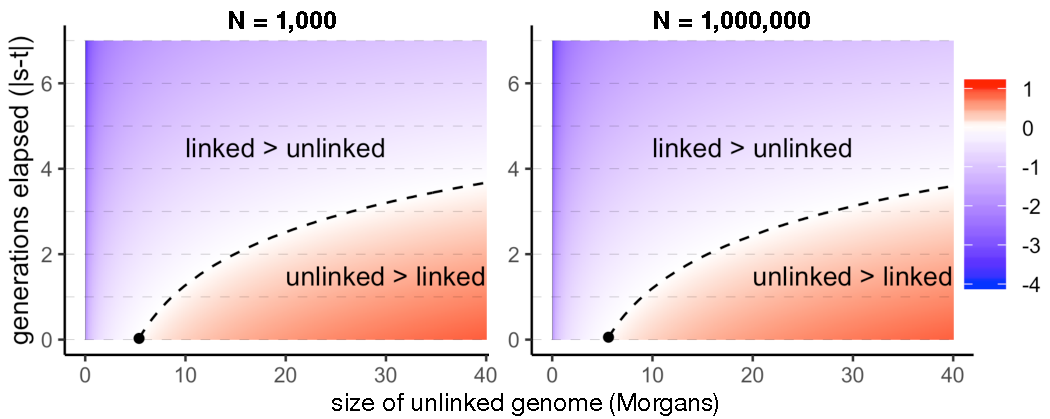
\includegraphics[]{./images/unlinked_linked_contributions.pdf}

  \caption{Here, we show the relative contributions of the linked and unlinked
    portions of the genome to the temporal autocovariance experienced by a
    neutral allele, for different generations elapsed (on the x-axis) and
    different map lengths of the unlinked genome (y-axis) for two different
    population sizes ($N=10^3$ and $N=10^6$). The color gradient is determined
    by the $\log_{10}$ value of the ratio of unlinked to linked contributions,
    the terms inside the braces in equation \eqref{eq:rel-contributions}. The
    dashed line indicates where the log ratio is zero, e.g. the relative
    contributions are equal; this was determined numerically. These assume LD
    is determined by mutation-drift-recombination balance
  \parencite{Tomoko_Ohta1971-hb}.}

  \label{fig:linked-unlinked}
\end{figure}

}


\subsection{Averaging covariance across multiple loci}

Thus far, our covariance assumes that a single neutral site is positioned in
the center of a region $R$ Morgans long, with selected sites uniformly
distributed along this region. In our simulations, however, we simulate a
region that contains many neutral sites which we average over in calculating
the temporal autocovariance. In this case, we average over the random distance
between a neutral site's position $n$ and a selected site's position $g$, which
is $c = |n - g|$, where $n, g \sim U(0, R)$. This random variable $c$ is
distributed according to the triangle distribution, $f(c) = 2(R-c) / R^2$; we
replace the uniform PDF in Equation \eqref{eq:exp-overselpos} with the triangle
density PDF and average over the distance between sites,

\begin{align}
  \frac{\E_n(\cov(\Delta p_t, \Delta p_s))}{\E_n(p_t(1-p_t)) } %&=  \frac{V_a(s)}{2L} \sum_{l=1}^L \int_{0}^R \E(\mathcal{R}^2_{t}(r(c))) (1-r(c))^{s-t} \frac{2(R-c)}{R^2} d c \label{eq:exp-overselpos} \\
  &= \frac{V_a(s)}{2} \int_0^R \E(\mathcal{R}_t^2(r(c))) \; (1-r(c))^{(s-t)} \frac{2(R-c)}{R^2} \,d c \\
  &= \frac{V_a(s)}{2} \mathcal{A}(R, t, s)
\end{align}
%
where $\E_n(\cdot)$ indicates we take the expectation also over neutral sites,
and we use $\mathcal{A}(R, t,s)$ to denote the average linkage disequilibrium
between selected and neutral sites that persists from generations $t$ to $s$
($t \le s$). Note that in calculating the standardized covariance above, we use
a ratio of expectations rather than the expectation of the ratio
\parencite{Bhatia2013-zy}.

\subsection{Empirically Calculating the Average LD Persisting Across Generations}
\label{ap:empirical-ld}

In the previous expressions for temporal autocovariance, we stepped through a
conceptual model for the average levels of linkage disequilibria between
neutral and selected sites that persists across $|s-t|$ generations
($\mathcal{A}(R, t,s)$), where the positions of selected and neutral sites are
randomly distributed along a chromosomal region. In systems with a known
recombination map and studies where linkage disequilibria can be calculated, we
have the recombination fraction $r_{i,j}$ and the pairwise linkage
disequilibria $\mathbf{R}^2_{i,j}$ between between two loci $i$ and $j$ (where
$\mathbf{R}^2$ is the $M \times M$ matrix of pairwise LD calculated at time
$t$). Since we do not \emph{a priori} know whether a site is selected or not,
we sum over all polymorphic $M$ loci, thus characterizing the average
linkage disequilibria in a region as

\begin{align}
  \label{eq:supp-emp-assoc}
  \overline{\mathcal{A}(t, s)} = \frac{2}{M(M-1)} \sum_{i=1}^{M} \sum_{j > i} \mathbf{R}_{i,j}^2  (1-r_{i,j})^{|t-s|}.
\end{align}
%
This sum is the empirical analog to the integral in Equation
\eqref{eq:multilocus-triangle}.

\subsection{The Strength of Unlinked and Non-gametic Associations}
\label{ap:strength-assoc}

Here, we characterize the contribution of completely genetically unlinked loci
segregating for fitness variation to the change in frequency of our neutral
allele. Across evolutionary replicates, there is no expected covariance between
the neutral allele an individual carries and their fitness ($\E(\Delta_{_H}
p_t)= \E(\cov(x_i, f_i)) = 0$); rather, for unlinked loci, chance associations
are created from the variance around this sampling process of neutral alleles
into individuals with varying fitness ($\var(\Delta_{_H} p_t)= \var(\cov(x_i,
f_i))$). As the neutral allele and fitness variation independently assort
themselves into individuals, the chance associations that form have a variance
given by $\var(\cov_i(x_i, f_i))$.  This has the form of the sampling variance
of a covariance, which for random variables $X$ and $Y$ is given by
\citeauthor{Kendall1994-gp} (\citeyear{Kendall1994-gp}, p. 472),

\begin{align}
  \var(\cov(X, Y)) &= \frac{(n-1)^2}{n^3} (\mu_{22} - \mu_{11}^2) + \frac{n-1}{n^3} (\mu_{20}\mu_{02} - \mu_{11}^2)  \\
                   &\text{where} \; \mu_{rs} = \E(X-\mu_X)^r(Y-\mu_Y)^s)
\end{align}
%
where $\mu_X$ and $\mu_Y$ are the means of $X$ and $Y$ respectively, and
the variance is taken over conceptual replicate populations and the covariance
is calculated over the individuals in a population.  Then, applying this to
our covariance $\Delta_{_H} p_1 = \cov_i(x_i, f_i)$,

\begin{align}
  \label{eq:strength-assoc}
  \var(\Delta_{_H} p_1) &= \nicefrac{1}{4}\var(\cov_i(x_i, f_i)) \nonumber \\
                     &= \frac{(N-1)^2}{4N^3} \left(\E[(x_i - p_0)^2 (f_i - 1)^2] - \E[(x_i - p_0) (f_i - 1)]^2 \right)+ \nonumber \\
                     &\;\;\;\;\;\; \frac{N-1}{4N^3} \left(\E[(x_i - p_0)^2] \E[(f_i - 1)^2] - \E[(x_i -p_0)(f_i-1)]^2\right) \nonumber \\
                     &= \frac{(N-1)}{4N^3} \var(x_i) \var(f_i) \nonumber \\
                     &\approx \frac{p_0(1-p_0) }{2N} \var(f_i).
\end{align}
%
Thus the chance covariances that form between the neutral alleles individuals
carry and their fitness have a variance proportional to
$\nicefrac{\var(f_i)}{2N}$. 

\paragraph{Non-gametic linkage disequilibrium's contribution to temporal autocovariance}
\label{ap:non-gametic}

\begin{figure}[!ht]
  \centering
  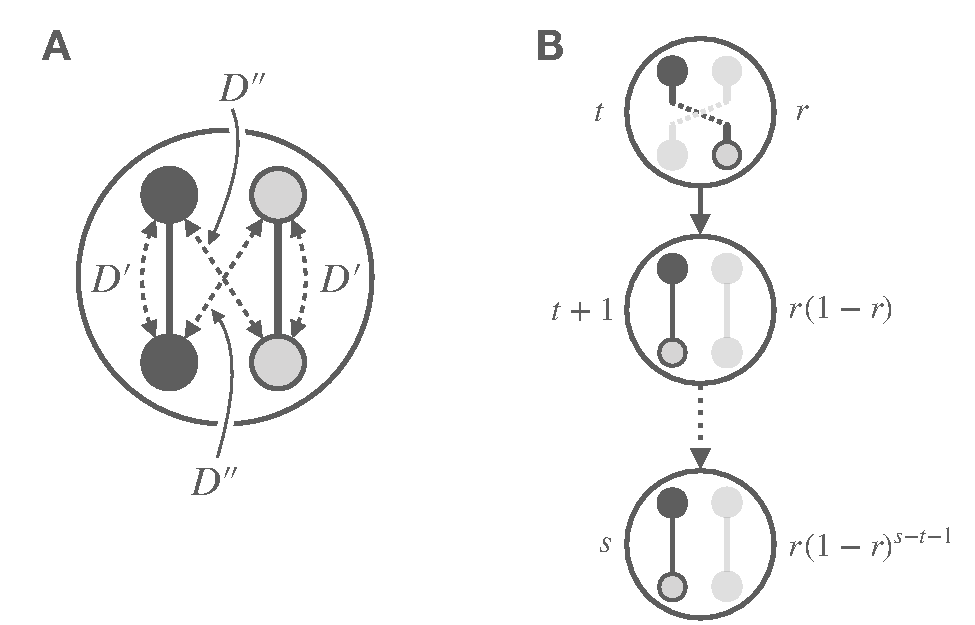
\includegraphics[scale=0.70]{./images/keynote-cartoons-wide.pdf}

  \caption{A: An illustration of gametic ($D'$) and non-gametic ($D''$) linkage
    disequilibria between two loci in a diploid. B: An illustration of how
    non-gametic linkage disequilibria in generation $t$ is converted to gametic
    linkage disequilibria through recombination (which happens with probability
    $r$, the recombination fraction between the two loci), and is then
    maintained until generation $s$ with probability $(1-r)^{s-t-1}$. The gray
    loci on the gray gamete indicate the homologous, but not tracked focal
    association. Overall, the covariance created by the conversion of non-gametic
    LD to gametic LD is $\E(D_{s}' D_{t}'') = r(1-r)^{s-t-1}\E\left((D_{t}'')^2\right)$.}

  \label{fig:ld-cartoon}
\end{figure}


Throughout the paper, we ignore the effects of non-gametic linkage
disequilibria, $D_{t,l}''$, the disequilibria that occurs between the two
gametes (maternal and paternal) at two loci (see Figure \ref{fig:ld-cartoon}
(A) for an illustration of gametic LD $D'$ and non-gametic LD $D''$). Following
Weir's equation for the sampling variance of non-gametic LD $D_{A/B}$ (p. 124,
\citeyear{Weir1996-mv}), the chance non-gametic disequilibrium that builds up
sampling $2N$ gametes into $N$ individuals is,

\begin{align}
  \E\left((D_{t,l}'')^2\right) = \var(D_{A/B})  = \frac{1}{2N} p_A (1-p_A) p_B (1-p_B).
  \label{eq:non-gametic}
\end{align}
%
Note the similar form to Equation \eqref{eq:strength-assoc} as both the
unlinked and non-gametic LD arise from the random sampling of alleles at
different loci into individuals.

There is no expected covariance between our gametic and non-gametic LD within a
generation $\E(D_{t,l}'', D_{t,l}')=0$, assuming random mating. However,
$\E(D_{t,l}'',D_{s,l}')>0$ for $s>t$, as a fraction of the non-gametic LD
may be converted into gametic LD in the next generation. Specifically,
following Santiago and Caballero (\citeyear{Santiago1995-hx}), we can write the
product of the non-gametic LD in generation $t$ with the gametic LD in
generation $s$ as

\begin{equation}
  \E(D_{t,l}'',D_{s,l}') = r(1-r)^{(s-t-1)} \E\left((D_{t,l}'')^2\right)
  \end{equation}
%
where a proportion $r$ the non-gametic LD in generation $t$ is converted into
gametic LD, and a proportion $(1-r)^{(s-t-1)}$ of this is carried forward
unbroken by recombination over the remaining $s-t-1$ generations (see Figure
\ref{fig:ld-cartoon}B for an illustration of this process).

In our analysis in the main text, we ignore these terms as $D_{t,l}''$ is
expected to be small due to its inverse dependence on $N$. However, these terms
are necessary for the analysis of looser linkage
\parencite{Santiago1995-hx,Santiago1998-bs}. 

\subsection{Connecting our model with the models of Robertson (1961) and Santiago and Caballero (1995, 1998)}
\label{ap:connecting-sc}

Here, we describe the models of \textcite{Santiago1995-hx,Santiago1998-bs},
relating their work on the long-run effective population size experienced by a
neutral allele where there is (1) unlinked heritable fitness variation (their
1995 paper), or (2) linkage, where fitness-determining sites are randomly
scattered along a chromosome (their 1998 paper). Overall, their models are
formulated in a quantitative genetics tradition, where the population genetic
dynamics at the selected loci are not explicitly modeled (although these links
are made more explicitly in their '98 paper). In contrast, in deriving our
expressions for temporal autocovariance and variances, we use a population
genetic approach, modeling the dynamics at selected sites (though we simplify
from the full multilocus treatment, e.g. we assume selected loci experience
independent sweeps and we ignore the LD between selected sites). We show that
we can reconcile the two approaches, and demonstrate that the temporal
autocovariance expressions we develop in our models are implicit in their
model. We also work through their expressions for $N_e$ with heritable
variance, because it represents a quite useful result but their original
presentation was spread across two papers (and a change in notation).

\paragraph{Santiago and Caballero's 1995 and 1998 models for $N_e$}

While our goal in the main text of our paper was to develop expressions for the
temporal variances and autocovariances in allele frequency change when there is
heritable fitness variation in the population, the goal of both the 1995 and
1998 Santiago and Caballero papers is to derive an expression for the long-run
$N_e$ when there is heritable variation for fitness in the population. In their
1995 paper, they find the effective population size for large $t$ (see p. 1018,
equation 16) to be

\begin{align}
  N_e &= \lim_{t \to \infty} \frac{p_0(1-p_0) - \var(p_{t-1})}{2(\var(p_t) - \var(p_{t-1}))}  \\
  N_e &= \frac{4N}{2 + V_n + Q^2 C^2}
\end{align}
%

where $C^2$ is the heritable variation for fitness ($V_A$ in our notation), and
$V_n$ is the non-heritable variation in offspring number (i.e. under a
Wright--Fisher model, $V_n \approx 2$). For a neutral locus completely unlinked
from fitness variation (the situation first considered by
\cite{Robertson1961-ho}), $Q = 1 + \nicefrac{G}{2} + (\nicefrac{G}{2})^2 +
(\nicefrac{G}{2})^3 + \ldots = \sum_{i=0}^\infty (\nicefrac{G}{2})^i =
\nicefrac{2}{(2 - G)}$ (\cite{Santiago1995-hx}, equation 17). \vb{Here, $G$
represents the decay rate of the additive genetic variance associated with a
particular haplotype.} Note that we've simplified their expressions by assuming
no assortative mating, and that we try to follow their notation as closely as
possible (consequently, the $Q$ here is unrelated to the $Q_{t,s}$ of the main
text).  \textcite{Santiago1995-hx} assume that continual artificial selection
maintains a constant level $C^2$ of fitness variation in the population each
generation, yet the \emph{particular} fitness backgrounds the neutral allele is
stochastically associated only contributes a fraction $G$ in the next
generation, $G^2$ in the generation after, and so on, as selection reduces
genetic variation for fitness (note: in their 1998 paper, they use $Z$ instead
of $G$). Similarly, the associations between the neutral and fitness
backgrounds decay at a rate $\nicefrac{1}{2}$ due to independent assortment.
Note that \textcite{Robertson1961-ho} assumed that the fitness backgrounds that
become stochastically associated with the neutral allele do not experience any
decay in their fitness variation ($G=1$); in this case, $Q = 2$ as Robertson's
work found. With an arbitrary amount of linkage between the focal neutral and
fitness backgrounds, \textcite{Santiago1998-bs} show that only $Q$ is affected,
and derive an expression for $Q$ that only depends on $G$ and the size of the
genome in Morgans, $L$ (equation 6, \citeyear{Santiago1998-bs}). 

In our main text, we model the temporal autocovariance created by heritable
fitness variation, which also impacts the cumulative variance in allele
frequency change $\var(p_t - p_0)$. To illustrate how our model connects with
theirs, below is the cumulative variance in allele frequency change for three
generations in their 1995 notation, with the corresponding changes in allele
frequency below,

\begin{align}
  \var(p_3 - p_0) = \E & \left( \bigg( \underbrace{S_1 + D_1 + H_1}_{\Delta p_1} + \right. \nonumber \\
                             & \underbrace{ (1-r) G S_1 + S_2 + D_2 + H_2}_{\Delta p_2} + \nonumber \\
                             & \left.  \underbrace{ (1-r)^2 G^2 S_1 + (1-r) G S_2 + S_3 + D_3 + H_3}_{\Delta p_3} \bigg)^2 \right).
                             % &  \underbrace{ (1-r)^2 G^2 S_1 + (1-r) G S_2 + S_3 + D_3 + H_3}_{\Delta p_3} + \nonumber \\
                             % &  \left. \underbrace{ (1-r)^3 G^3 S_1 + (1-r)^2 G^2 S_2 + (1-r) G S_3 + S_4 + D_4 + H_4}_{\Delta p_4} \bigg)^2 \right) \nnn  \\
    \label{eq:sc-var4}
\end{align}
%
Grouping terms by the generation that the initial association was formed, we
see how \textcite{Santiago1995-hx} define the $Q_i$ terms in their notation,

\begin{align}
  \var(p_3 - p_0) = \E & \left( \bigg( \underbrace{S_1(1 + (1-r) G + (1-r)^2 G^2)}_{\text{creation and persistence of generation 1 associations} \;\; := \; S_1 Q_3} \right. +  D_1 + H_1+ \nonumber \\
                       & \underbrace{S_2(1 + (1-r) G)}_{\text{creation and persistence of generation 2 associations} \;\; := \; S_2 Q_2}+ D_2 + H_2 + \nonumber \\
                       &  \underbrace{S_3}_{\text{creation of generation 3 associations} \;\; := \; S_3 Q_1  }\left. + D_3 + H_3 \bigg)^2 \right). &
    \label{eq:scr-var2}
\end{align}
%
since the associations created in generation $i$ ($ 0 < i \le t$) persist with
probability $(1-r)^{t-i}$, with proportion $G^{t-i}$ of its original fitness
variation in generation $t$. In general, the cumulative impact of the
associations formed $i$ generations ago has coefficient $Q_i =
\sum_{j=0}^{i-1} (1-r)^j G^j$. Using these $Q_i$ terms simplifies this equation
to

\begin{align}
  \var(p_4 - p_0) &= \E \left( \bigg(  S_1 Q_4 + D_1 + H_1 + S_2 Q_3 + D_2 + H_2 + \right. \nonumber \\
                  & \;\;\;\;\;\;\;\;\;\;\; \left. S_3 Q_2 + D_3 + H_3 + S_4 Q_1 + D_4 + H_4 \bigg)^2 \right)
                  % &= \sum_{i=1}^4 \var(\Delta_{_N} p_i) + \var(\Delta_{_M} p_i) + \sum_{i,j}^4 \cov(\Delta_{_H} p_i, \Delta_{H} p_j)
\end{align}
%
or, in general,

\begin{align}
    \var(p_t - p_0) &= \sum_{i=1}^t \E(D_i^2) + \E(H_i^2) + Q_{t-i+1}^2 E(S_i^2).
\end{align}

Then, Santiago and Caballero (1995) note that assuming $V_n$, $C^2$, and
population size $N$ are constant across generations, the magnitude of all of
the effects $\E(D_i^2)$, $\E(H_i^2)$, and $\E(S_i^2)$ are constant across all
generations (for all $i$, so we omit the $i$ subscript for these terms), except
for a geometric decay due to drift at a rate $(1-\nicefrac{1}{2N_e})$ per
generation that effects all terms. Such that, when we include the decay in the
variance due to drift,

\begin{align}
  \var(p_t - p_0) &= \sum_{i=1}^t \left(\E(D^2) + \E(H^2) + Q_{i}^2 E(S^2) \right) \left( 1 - \frac{1}{2N_e} \right)^{t-i}
  \label{eq:var-sc}
\end{align}
%
(cf. p. 1018 of \cite{Santiago1995-hx}). In the long run, the variance in the
neutral allele's frequency change hits a balance. Many copies of the neutral
allele segregating in the population are on fitness backgrounds it has recently
become stochastically associated with, as segregation and recombination have
not broke these associations apart. A few copies of the neutral allele are on
fitness backgrounds they became associated with many generations ago, that have
by chance survived to remain associated. In all cases, the effect these
associations have on present-day allele frequency change is weakened by the
fact that natural selection has reduced the genetic variance of these fitness
backgrounds. Since the long-run variance in allele frequency under drift in a
Wright--Fisher population is

\begin{align}
  \var(p_t) = p_0(1-p_0) \left[1 - \left(1 - \frac{1}{2N}\right)^t \right].
  \label{eq:sc-Ne}
\end{align}

One can estimate the effective population size $N_e$ using the observed
difference in variances $\var(p_t)$ and $\var(p_{t-1})$. (Note that this is
a different long-run effective population size used by others, $N_e =
p_0(1-p_0) t / (2\var(p_t - p_0))$, \cite{Crow1970-wm}) Santiago and
Caballero use Equation \eqref{eq:sc-Ne}, taking the difference $\var(p_t) -
\var(p_{t-1})$ and rearranging to end up with the large $t$ estimator of $N_e$, 

\begin{align}
  N_e = \frac{p_0(1-p_0) - \var(p_{t-1})}{2(\var(p_t) - \var(p_{t-1}))}
\end{align}
%
(cf. p. 1018, \cite{Santiago1995-hx}). Rearranging,

\begin{align}
  2N_e(\var(p_t) - \var(p_{t-1})) &= p_0 (1-p_0) - \var(p_{t-1}) \nonumber \\
  2N_e \var(p_t) - 2N_e \var(p_{t-1}) + \var(p_{t-1}) &= p_0(1-p_0) \nonumber \\
  2N_e \bigg(\var(p_t) - \var(p_{t-1}) \left(1 - \frac{1}{2N_e} \right)\bigg) &= p_0(1-p_0).
  \label{eq:sc-N}
\end{align}

This very conveniently simplifies the sum in Equation \eqref{eq:var-sc}, as we
can show with the case of $t=3$,

\begin{align}
  \var(p_3) = &\left(\E(D^2)+\E(H^2)+Q_1^2 \E(S^2)\right) \left(1-\frac{1}{2 N_e}\right)^2 + \nonumber \\
              &\left(\E(D^2)+\E(H^2)+Q_2^2 \E(S^2)\right) \left(1-\frac{1}{2 N_e}\right) + \nonumber \\
              &\;\E(D^2)+\E(H^2)+Q_3^2 \E(S^2) \nonumber \\
  \var(p_2)\left(1-\frac{1}{2N_e}\right) = &\left(\E(D^2)+\E(H^2)+Q_1^2 \E(S^2)\right) \left(1-\frac{1}{2N_e}\right)^2 + \nonumber \\
                                         &\;(\E(D^2)+\E(H^2)+Q_2^2 \E(S^2)) \left(1-\frac{1}{2N_e}\right) \nonumber \\
  \var(p_3) - \var(p_2)\left(1-\frac{1}{2N_e}\right) = &\E(D^2) + \E(H^2) + Q_3^2 \E(S^2) \nnn
\end{align}

or, generally, 

\begin{align}
  \var(p_t) - \var(p_{t-1})\left(1-\frac{1}{2N_e}\right) &= \E(D^2) + \E(H^2) + Q_t^2 \E(S^2)
\end{align}
%
Inserting this into Equation \eqref{eq:sc-N}, the long-run effective population
size can be written as

\begin{align}
  N_e &= \frac{p_0(1-p_0)}{2\bigg(\var(p_t) - \var(p_{t-1}) \left(1 - \frac{1}{2N_e} \right)\bigg)} \nonumber \\
      &= \frac{p_0(1-p_0)}{2\left( \E(D^2) + \E(H^2) + Q_\infty^2 \E(S^2) \right)}
  \label{sc:ne-eqn}
\end{align}
%
where $Q_\infty = 1 + \nicefrac{1}{2} + \nicefrac{1}{4} + \ldots = 2$ in
Robertson's (\citeyear{Robertson1961-ho}) model, and $Q_\infty = 1/(1 - G
(1-r))$ in Santiago and Caballero's (1995) model. (Note: $r$ here represents
the recombination fraction between fitness variation and neutral sites, which
differs from \textcite{Santiago1995-hx} equation 17, where $r$ represents the
correlation between parental fitness).

Then, \textcite{Santiago1995-hx} show,

\begin{align}
  \E(S^2) &= \frac{p_0(1-p_0)}{2N} C^2 \\
  \E(D^2) &= \frac{p_0(1-p_0)}{2N} \frac{V_n}{4} \\
  \E(H^2) &= \frac{p_0(1-p_0)}{2N} \frac{1}{2}
\end{align}
%
(cf. \cite{Santiago1995-hx}, equation 11). Inserting these into Equation
\eqref{sc:ne-eqn}, we have

\begin{align}
  N_e &= \frac{4N}{2 + V_n + 4 Q_\infty^2 C^2}
\end{align}
%
which is a simplified version of Santiago and Caballero's equation 16, and
which further simplifies to $N_e = N$ when $V_n = 2$ and $C^2 = 0$, the
effective population size of a Wright--Fisher population of $N$ hermaphroditic
individuals.


\paragraph{The covariances caused by fitness associations}

With an understanding now of the basics of Santiago and Caballero's (1995,
1998) models, how they connect to our notation, and how they reach their
expression for the long-run effective population size, we turn now to finding
the temporal autocovariances implicit in their model. We start by looking at
the variance in allele frequency between generations $0$ and $4$ (Equation
\eqref{eq:sc-var4}), including an additional generation so the pattern is
clearer later,

\begin{align}
  \var(p_4 - p_0) = \E & \left( \bigg( \underbrace{S_1 + D_1 + H_1}_{\Delta p_1} + \right. \nonumber \\
                             & \underbrace{ (1-r) G S_1 + S_2 + D_2 + H_2}_{\Delta p_2} + \nonumber \\
                             &  \underbrace{ (1-r)^2 G^2 S_1 + (1-r) G S_2 + S_3 + D_3 + H_3}_{\Delta p_3} + \nonumber \\
                             &  \left. \underbrace{ (1-r)^3 G^3 S_1 + (1-r)^2 G^2 S_2 + (1-r) G S_3 + S_4 + D_4 + H_4}_{\Delta p_4} \bigg)^2 \right). \nnn 
\end{align}

The cross-terms like $\E(D_1 D_2)$, $\E(H_1 D_1)$ and $\E(S_1 S_2)$ are all expected
products of independent random variables, where the expectation of each random
variable is zero, and consequently are all zero. The only non-zero cross terms
are products of $\E(S_i^2)$. When we look at the covariances with the allele
frequency change in the initial generation and a later generation $s$,
$\cov(\Delta_{_H} p_1, \Delta_{_H} p_s)$,

\begin{align}
  \cov(\Delta_{_H} p_1, \Delta_{_H} p_1) &= \var(\Delta_{_H} p_1) = \E(S_1^2) \\
  \cov(\Delta_{_H} p_1, \Delta_{_H} p_2) &= \frac{\E(S_1^2) G}{2} (1-r) \\
  \cov(\Delta_{_H} p_1, \Delta_{_H} p_3) &= \frac{\E(S_1^2) G^2 }{2}(1-r)^2\\
  \cov(\Delta_{_H} p_1, \Delta_{_H} p_4) &= \frac{\E(S_1^2) G^3 }{2} (1-r)^3
\end{align}
%
where the $\nicefrac{1}{2}$ coefficient comes from the fact that in Santiago
and Caballero's work, the $\E(S_1^2)$ products represent \emph{both} the
$\cov(\Delta_{_H} p_t, \Delta_{_H} p_s)$ and $\cov(\Delta_{_H} p_s, \Delta_{_H}
p_t)$ terms, so a single temporal autocovariance in our notation is half 
their joint covariance term.

However, if our reference generation is different, say 2, the associations from
earlier generations that have persisted to that generation can also lead to
covariances to later generations. Looking at the covariances 

\begin{align}
  \cov(\Delta_{_H} p_2, \Delta_{_H} p_2) &= \frac{\E(S_2^2) + \E(S_1^2) (1-r) G}{2} \\
  \cov(\Delta_{_H} p_2, \Delta_{_H} p_3) &= \frac{\E(S_2^2) G  + \E(S_1^2) (1-r) G^2}{2} (1-r) \\
  \cov(\Delta_{_H} p_2, \Delta_{_H} p_4) &= \frac{\E(S_2^2) (1-r) G^2 + \E(S_1^2) (1-r)^2 G^3}{2} (1-r)2.
\end{align}

Likewise, the covariances $\cov(\Delta_{_H} p_3, \Delta_{_H} p_s)$ include the
associations that persist from earlier generations. In general, 

\begin{align}
  \cov(\Delta_{_H} p_t, \Delta_{_H} p_s) = \frac{1}{2}\sum_{i=1}^{t} \E(S_i^2) \left(G (1-r)\right)^{t + s - 2i}, \; \; \text{for} \; \; t \le s.
  \label{eq:sc-cov}
\end{align}

This expression is more complex than our expression for temporal autocovariance
because its modeling the LD in generation $t$ as it builds up from generations
1 to $t$. In contrast, our expressions for covariance incorporate all of this
build up of LD as the initial LD term $\E(\mathcal{R}_t)$ (for a single locus case). This
expression for autocovariance implied by Santiago and Caballero's (1995) work
matches our expression for autocovariance (for a single locus) when the
arbitrary first generation is $t$ rather than 1

\begin{align}
  \cov(\Delta_{_H} p_t, \Delta_{_H} p_s) &= \frac{\E(S_t^2)G^{s-t}}{2}  (1-r)^{s - t}, \; \; \text{for} \; \; t \le s.
\end{align}

Using the expression for $\E(S_t^2)$ (equivalent to $\var(\Delta_{_H} p_t)$ in
our notation) derived in Appendix Section \ref{ap:strength-assoc}, 

\begin{align}
  \frac{\cov(\Delta_{_H} p_t, \Delta_{_H} p_s)}{p_t(1-p_t)} &= \frac{C^2 G^{s-t}}{4N}  (1-r)^{s - t}, \; \; \text{for} \; \; t \le s.
\end{align}

This is analogous to Equation \eqref{eq:multilocus-cov-sum} for a single
locus, where $C^2 G^{s-t}$ is the additive variation in generation $s$
(equivalent to our $V_a(s)$), and the factor $\nicefrac{1}{2N}$ represents the
chance build up of LD between the neutral site and an unlinked fitness background.
In our expression, we condition on existing linkage disequilibrium $\E(\mathcal{R}_t^2)$
between the neutral site and its fitness background, whereas they assume a
buildup of linkage disequilibria to a drift-recombination equilibrium. We can
see this by returning to the $\Delta_{_H} p_4$ term of Equation
\eqref{eq:sc-var4},

\begin{align}
  \var(\Delta_{_H} p_4) &= \E\left( (1-r)^3 G^3 S_1 + (1-r)^2 G^2 S_2 + (1-r) G S_3 + S_4 + D_4 + H_4\right)^2  \\
                        &= (1-r)^5 G^5 \E(S_1^2) + (1-r)^4 G^4 \E(S_2^2) + (1-r)^2 G^2 \E(S_3)^2 + \E(S_4^2) 
\end{align}
%
where following Santiago and Caballero's (\citeyear{Santiago1995-hx}, p. 1018)
approach, we can replace each $\E(S_i)$ with $\E(S_i^2) =
\E(S^2)(1-\nicefrac{1}{2N})^{i-1}$ and let $G=1$ as we focus on the buildup of
LD. This gives us the general equation, 

\begin{align}
  \var(\Delta_{_H} p_t) = \E(S^2) \sum_{i=1}^t (1-r)^{2i} \left(1-\frac{1}{2N}\right)^{i-1}
\end{align}
%
and taking this geometric series to infinity converges (since $(1-r)^2
(1-\nicefrac{1}{2N}) < 1$) and replacing $\E(S^2)$ with the chance associations
that build up gametes sampled into individuals (Equation
\eqref{eq:strength-assoc}),

\begin{align}
  \E((\Delta_{_H} p_\infty)^2) &= \E(S^2) \sum_{i=1}^\infty (1-r)^{2i} \left(1-\frac{1}{2N}\right)^{i-1} \nonumber \\
                             &= \frac{\E(S^2)}{1-\nicefrac{1}{2N}} \sum_{i=1}^\infty \left((1-r)^2 \left(1-\frac{1}{2N}\right)\right)^{i} \nonumber \\
                             &= \frac{C^2 p_0(1-p_0)}{1-\nicefrac{1}{2N}} \frac{1}{1-(1-r)^2 (1-\nicefrac{1}{2N})}.
\end{align}
% 
When we assume $r \to 0$ and $1/N \to 0$ and $Nr$ is a constant, this gives us

\begin{align}
  \E(\mathcal{R}^2) = \frac{\E((\Delta_{_H} p_\infty)^2)}{C^2 p_0(1-p_0)} &\approx \frac{1}{1 + 4Nr}
\end{align}
%
which is analogous to the $\E(\mathcal{R}^2)$ measure of linkage disequilibrium,
standardized to rescale the fitness variation. The right-hand side is identical
to \citeauthor{Sved1971-dv}'s identity by descent equilibrium $\E(\mathcal{R}^2)$ under
drift-recombination balance (\citeyear{Sved1971-dv}). Note that our expression
can be recovered from Equation \eqref{eq:sc-cov} when the reference generation
$t \to \infty$ such that the LD hits its equilibrium level,

\begin{align}
  \frac{\cov(\Delta_{_H} p_t, \Delta_{_H} p_s)}{p_0(1-p_0)} &= \frac{1}{2} \underbrace{C^2 G^{s-t}}_{V_A(s)} \underbrace{\frac{1}{1 + 4Nr}}_{\E(\mathcal{R}_t^2)} (1-r)^{s-t}
\end{align}
%
which is identical to our expression for temporal autocovariance when initial
LD is due to a neutral drift-recombination balance, and the change in $V_A$
during selection is modeled as a geometric decay at rate $G$.  Note that the
terms in underbraces indicate the corresponding terms in Equation
\eqref{eq:multilocus-cov-sum} for a single locus.

\subsection{Multilocus simulation details}
\label{sec:supp-ml-sim}


\paragraph{Targeting an initial level of Additive Genetic Variation}
\label{sec:supp-ml-sim-va}

We choose $\theta$ for the coalescent simulations to target a total number of
segregating sites $L + M$, where $L$ is the number of selected sites (a
parameter we vary in our multilocus simulations), and at least $M=200$ randomly
placed neutral sites over which we can calculate the temporal autocovariance.
Then, the total number of target sites $M+L$ is then inflated by a factor of
1.5 to ensure a sufficient number of sites given the random mutation process.
The $L$ selected sites are randomly chosen from the segregating sites, and all
remaining mutations are neutral. Thus, using \citeauthor{Watterson1975-kt}'s
expression for the expected number of segregating sites under the coalescent
(\citeyear{Watterson1975-kt}), we have $\theta = 1.5(M+L) / (\gamma +
\log(2N))$ where $\gamma \approx 0.577$ is Euler's Gamma. Each of the $L$
selected sites is given a random effect size of $\pm \alpha$ with equal
probability, where we choose by targeting a specific level additive genic
variation $V_a = 2 \alpha^2 \sum_l^L p_l(1-p_l) = \alpha^2 SSH_L$ where $SSH_L
= 2 \sum_l^L p_l(1-p_l)$ is the sum of site heterozygosity of the $L$ neutrally
evolving sites that will be selected once selection begins. Under neutrality,
$\E(SSH_L) = \theta_L = L/(\gamma + \log(2N))$. Then, we set $\alpha =
\sqrt{\nicefrac{V_a}{\theta_L}}$. We empirically validate that our target genic
variation is close to the empirically observed level.

\paragraph{Choosing the simulation parameter range}
\label{sec:supp-ml-sim-param}

We simulate over a grid of parameter ranges, varying the number of loci $L$,
the target additive genic variation $V_a$ in the region (by varying $\alpha$),
and the recombination map length of the region $R$ in Morgans. We have varied
these parameters over ranges that encompass a wide range likely to be
encountered in natural populations. To do this, we found that additive genetic
variation for lifetime reproductive success varied over orders of magnitude,
from 0 (e.g. in male red deer, \textcite{Kruuk2000-xt}) to ~1.1 in male
red-billed gull \parencite{Teplitsky2009-oj}. These values of additive genetic
variation are for the entire genome (we write these as $V_{A,GW}$, where $GW$
indicates genome-wide); our simulations model a region of varying map length.
We expect most recombination map lengths to be roughly over the scale of $5-50$
Morgans in length, and we chose to investigate how temporal autocovariance
behaves across a spectrum of recombination, from a completed linked region
($R=0$), to the scale over which a strong classic hardsweeps could affect
diversity (0.5 centiMorgans) to a region where the ends are approximately
unlinked (4.5 Morgans), overall giving us a parameter range of $R \in \{0,
0.005, 0.01, 0.05, 0.1, 0.5, 1.5, 4.5\}$.  Over this grid of our region
recombination map lengths, and the total organism recombination map lengths, we
get a rough estimate of the number of regions we would expect with this level
of recombination in the organism's total genome, imagining homogeneous
recombination rate, by taking $G/R$. Using this estimate of the number of
regions in the genome, we calculate the genetic variation per region over our
grid of parameters as $\nicefrac{V_{A,GW} R}{G}$, and target a level of
additive genic variation per region $V_a$ equal to this regional additive
genetic variation $V_A$. From preliminary simulations, we had found we can not
detect much temporal autocovariance below $V_a < 0.001$ with the initial level
of linkage disequilibrium from mutation-drift balance, so we ignore parameters
less than this value (other than $V_a=0$ as a control). Additionally, to reduce
the number of simulations, we exclude $V_a > 0.1$ as this only excludes a small
region of the parameter grid and preliminary simulations demonstrated the
behavior of temporal autocovariance with high $V_a$ is evident with the
included values. Overall, this gives us a spectrum of target additive genic
variation per region of $V_a \in \{0.001, 0.002, 0.005, 0.01, 0.02, 0.05, 0.08,
0.1\}$.  Note that to prevent our plots from being too dense, we include only a
representative subset of this parameter grid in our figures.


\subsection{Accounting for allele frequency sampling noise}
\label{sec:sampling}

In practice, one will calculate the temporal variance-covariance matrix on
allele frequency trajectories calculated from sampled chromosomes from the
population. We assume a binomial sampling process, where $n$ chromosomes are
sampled from the population such that $\widetilde{p} = \nicefrac{X}{n}$, and $X
\sim \textrm{Binom}(p, n)$. We can then write $\widetilde{p}_t = p_t +
\varepsilon_t$, and our covariances can be written as

\begin{align}
  \cov(\Delta \widetilde{p_t}, \Delta \widetilde{p_s}) &= \cov(\widetilde{p}_{t+1} - \widetilde{p}_{t}, \widetilde{p}_{s+1} - \widetilde{p}_{s}) \nonumber \\
  &= \cov(p_{t+1} + \varepsilon_{t+1} - p_{t} - \varepsilon_{t}, p_{s+1} + \varepsilon_{s+1} - p_{s} - \varepsilon_{s}).
\end{align}
%
Note this simplifies to

\begin{align}
  \cov(\Delta \widetilde{p_t}, \Delta \widetilde{p_s}) &= \cov(p_{t+1} - p_{t}, p_{s+1} - p_{s}) \; \; \mathrm{if} \;\; |t-s| > 1,
\end{align}
%
since in these cases, the sampling noise at a timepoint is not shared between
the estimated allele frequency changes. However, if $|t - s| = 1$ the sampling
noise from timepoint $t+1$ is shared, biasing the sample estimate of
covariance:

\begin{align}
\cov(\Delta \widetilde{p_t}, \Delta \widetilde{p}_{t+1}) 
  &= \cov(p_{t+1} + \varepsilon_{t+1} - p_{t} - \varepsilon_{t}, p_{t+2} + \varepsilon_{t+2} - p_{t+1} - \varepsilon_{t+1}) \nonumber \\
  &= \cov( \Delta p_{t} + \varepsilon_{t+1} - \varepsilon_{t}, \Delta p_{t+1} + \varepsilon_{t+2} - \varepsilon_{t+1}) \nonumber \\
  &= \cov(\Delta p_{t}, \Delta p_{t+1}) - \var(\varepsilon_{t+1}).
\end{align}
%
Similarly, the variance ($t = s$) is biased, as it is impacted by the binomial
sampling noise too,
%

\begin{align} 
  \var(\Delta \widetilde{p_t}) &= \cov( \Delta p_{t} + \varepsilon_{t+1} - 
      \varepsilon_{t}, \Delta p_{t} + \varepsilon_{t+1} - \varepsilon_{t}) \nonumber \\ 
                               &= \var( \Delta p_{t} ) + \var(\varepsilon_{t+1}) +
\var(\varepsilon_{t}) \end{align}
%
In practice, these covariances are calculated over loci in a region or across the
entire genome. We assume that the tracked allele has been randomly swapped
(e.g. the tracked allele frequency is not systematically the minor, major, or
reference allele), such that $\E(\Delta p_{t,l}) = 0$ for all $t$ and $l$. Then,
the unbiased covariance estimate as calculated over loci is

\begin{align}
  \frac{1}{L} \sum_{l=1}^L \left(\Delta p_{t,l} \Delta p_{t+1,l} \right)  &=
  \frac{1}{L} \sum_{l=1}^L \Delta \widetilde{p}_{t,l} \Delta \widetilde{p}_{t+1,l}
  + \frac{1}{L} \sum_{l=1}^L \varepsilon_{t+1,l}^2.
\end{align}
%
Then, we can use an unbiased plugin estimate of the frequency sampling variance
$\E(\varepsilon_{t+1,l}^2) = \V(\varepsilon_{t+1,l}) =
\nicefrac{p_{t+1,l}(1-p_{t+1,l})}{(n_{t,l}-1)}$ \parencite[p. 191]{Nei1987-bx}
to estimate these bias terms, and add or subtract them from the estimator
accordingly. Accounting for finite sampling, the unbiased sample
variance-covariance matrix now has elements:

\begin{align}
  \label{eq:corrected-var}
  Q_{t,t+1} &=
  \frac{1}{L} \sum_{l=1}^L \Delta \widetilde{p}_{t,l} \Delta \widetilde{p}_{t+1,l}
  + \frac{1}{L} \sum_{l=1}^L \frac{p_{t+1,l}(1-p_{t+1,l})}{n_{t+1,l} - 1},
\end{align}
and variance

\begin{align}
  \label{eq:corrected-cov}
  Q_{t,t} &=
  \frac{1}{L} \sum_{l=1}^L (\Delta \widetilde{p}_{t,l})^2
  - \frac{1}{L} \sum_{l=1}^L \frac{p_{t,l}(1-p_{t,l})}{n_{t,l} - 1}
  - \frac{1}{L} \sum_{l=1}^L \frac{p_{t+1,l}(1-p_{t+1,l})}{n_{t+1,l} - 1}.
\end{align}

In Section \ref{sec:ml-sim-res}, we used population frequencies in
introducing the method of moments estimators of $\widehat{V_A(1)}$ and
$\widehat{N}$. Here, we discuss the performance of these estimators with sample
allele frequencies. Our simulations are identical to those described in Section
\ref{sec:ml-sim}, except we have increased the target number of neutral sites
in each region so it is around $10,000$. We mimic sampling of $n=\{50, 100,
200, 500\}$ chromosomes from the population, and use the bias-corrected
sample variance-covariance matrix in the method-of-moments approach described
in Section \ref{sec:meth-moments} to estimate $\widehat{V_A(1)}$ and
$\widehat{N}$.

In Figure \ref{fig:mom-fits-both-finite}, we show the performance of our
estimators in the case where $n=100$ chromosomes have been sampled from the
population. Overall, there are two important differences compared with Figure
\ref{fig:mom-fits-both} of the main text. First, while the estimator
$\widehat{V_A(1)}$ performs well for high levels around $V_A \sim 0.1$, the
variance around the estimator increases significantly as $V_A$ grows weaker.
As the covariances are proportional to $\nicefrac{V_A}{R}$, sampling noise
grows larger than the theoretical temporal autocovariance as $V_A$ become weaker.
Then, one cannot discriminate against the chance covariances formed by the
sampling process from the temporal autocovariance created by linked selection
without either a large sample size or more timepoints. Second, the approach
underestimates $V_A(1)$ for very loose linkage ($R > \nicefrac{1}{2}$). This is
another consequence of the first problem; as sampling noise grows equal, or
larger than the magnitude of temporal autocovariance, the estimation procedure
performs poorly. As the linkage becomes more loose, the magnitude of temporal
autocovariance grows weak relative to the sampling noise, and this noise can be
partially absorbed by $\widehat{N}$. This effect can be somewhat ameliorated by
calculating the sample variance-covariance matrix over a shorter region of the
genome such that $R$ is smaller (as long as SNP density is sufficient), or by
increasing the sample size. Finally, the estimation of effective population
size shown in Figure \ref{fig:mom-fits-both-finite} are also affected by $V_A$,
as discussed in Section \ref{sec:meth-moments} (though the effect is obscured
by the sampling noise): high levels of $V_A$ in regions with low recombination
generally lead to underestimates of $\widehat{N}$.

To understand how sample size affects the method-of-moments estimators, Figure
\ref{fig:mom-relative} depicts median relative error of $\widehat{V_A(1)}$ and
$\widehat{N}$ for various sample sizes.


\begin{figure}
  \centering
  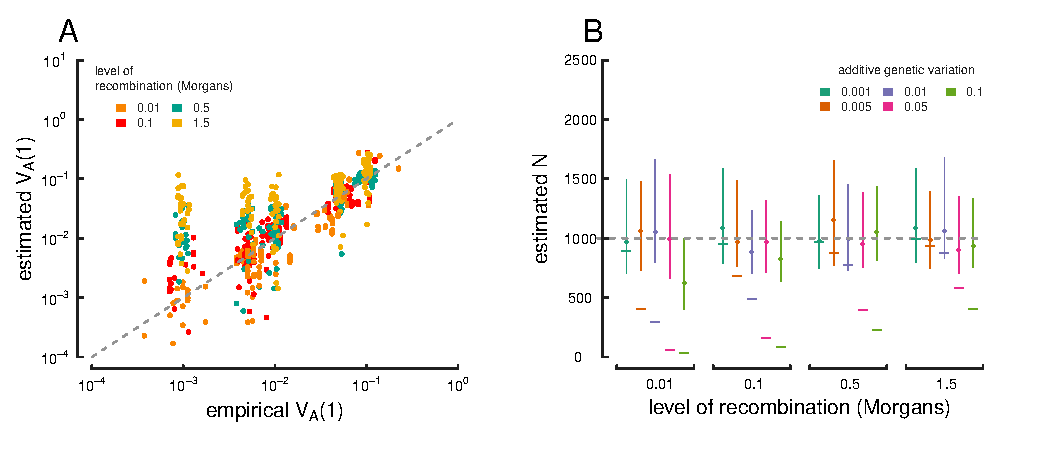
\includegraphics{./images/mom-fits-both-alt-finite.pdf} 

  \caption{True parameter values and estimates using the method-of-moments
      approach on sample ($n=100$ chromosomes) multilocus simulation data;
      these figures are analogous to Figure \ref{fig:mom-fits-both} in the main
      text, except the estimators have been calculated on sample, rather than
      population frequency data. (A) The true $V_A(1)$ (x-axis) and
      $\widehat{V_A(1)}$ estimated from the sample variance/covariance matrix
      (y-axis) for each simulation replicate across different levels of
      recombination (indicated by each point's color). (B) Estimated
      drift-effective population size ($\widehat{N}$) across a range of
      simulations with different levels of additive genetic variance and
      recombination. Each point denotes the median, with lines denoting the
      interquartile range. A simple temporal estimate of the effective
      population size, estimated with accounting for the effects of selection,
  is averaged for each replicate and plotted as a dash. The true value ($N =
  1,000$) is shown with the dashed gray line.}

\label{fig:mom-fits-both-finite}
\end{figure}


\begin{figure}
  \centering
  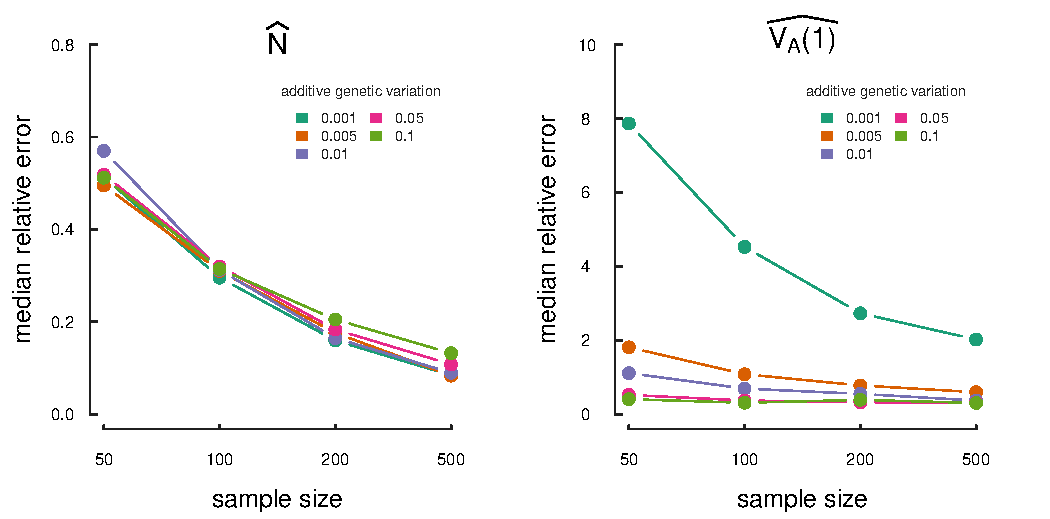
\includegraphics{./images/supp-relative-error.pdf} 

  \caption{The median relative estimation error, over 30 replicate simulations,
  of the method of moments estimator for drift effective population size
($\widehat{N}$) and the initial additive genetic variance ($\widehat{V_A(1)}$).
} 

\label{fig:mom-relative}
\end{figure}




\newpage
\subsection{Appendix Figures}

\subsubsection{Validation of simulation routine}

\begin{figure}[!ht]
  \centering
  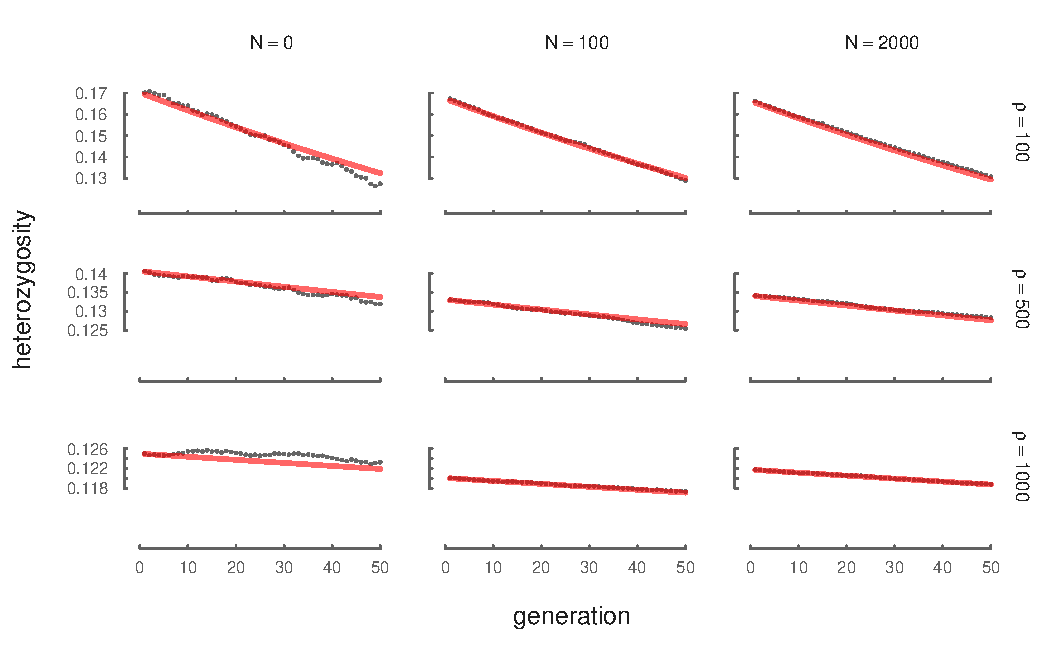
\includegraphics{./images/supp-het-neutral.pdf}

\caption{The neutral decay of heterozygosity due to drift, averaged across 100
replicates and a variety of $N$ and $\rho$ levels. The red line is the
theoretical expectation $H_t = H_1 (1-1/(2N))^{t-1}$.}

\label{fig:het-neut}
\end{figure}


\begin{figure}[!ht]
  \centering
  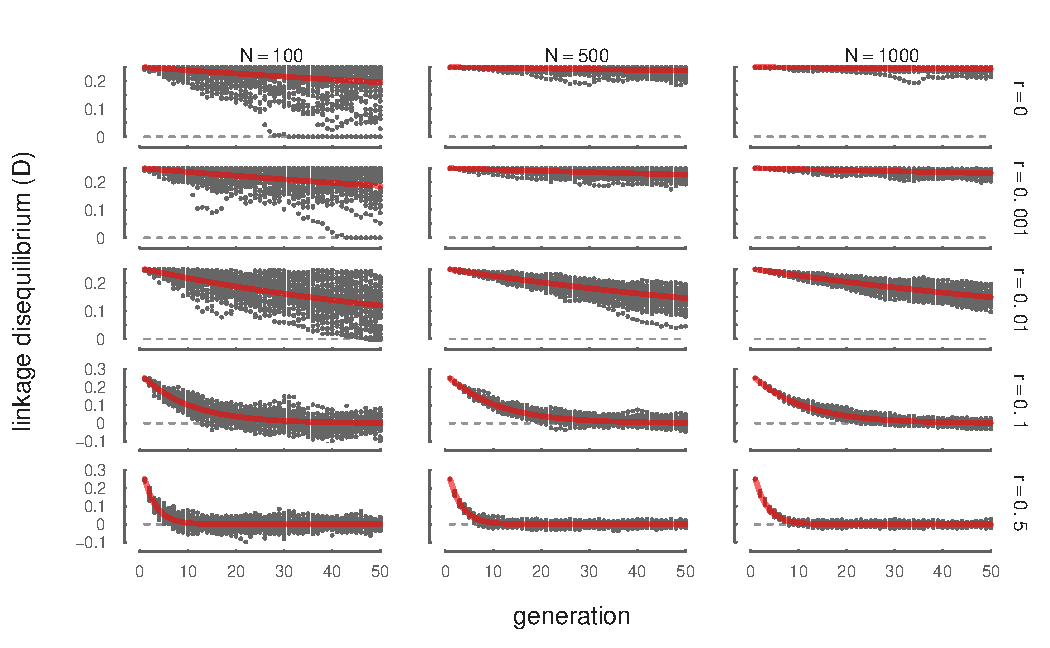
\includegraphics{./images/supp-ld-neutral.pdf}

  \caption{The decay of LD between neutral sites due to recombination, across
    100 replicates and a variety of $V_A$ and $R$ levels. The initial
    population is created to have an artificial level of initial LD, with half
    the gametes carrying all derived alleles, and the other half carrying all
  ancestral alleles. The red line is the theoretical expectation $D_t = D_1 (1-1/(2N))^{t-1} (1-r)^{t-1}$.}

  \label{fig:ld-neut}
\end{figure}


\begin{figure}[!ht] \centering
  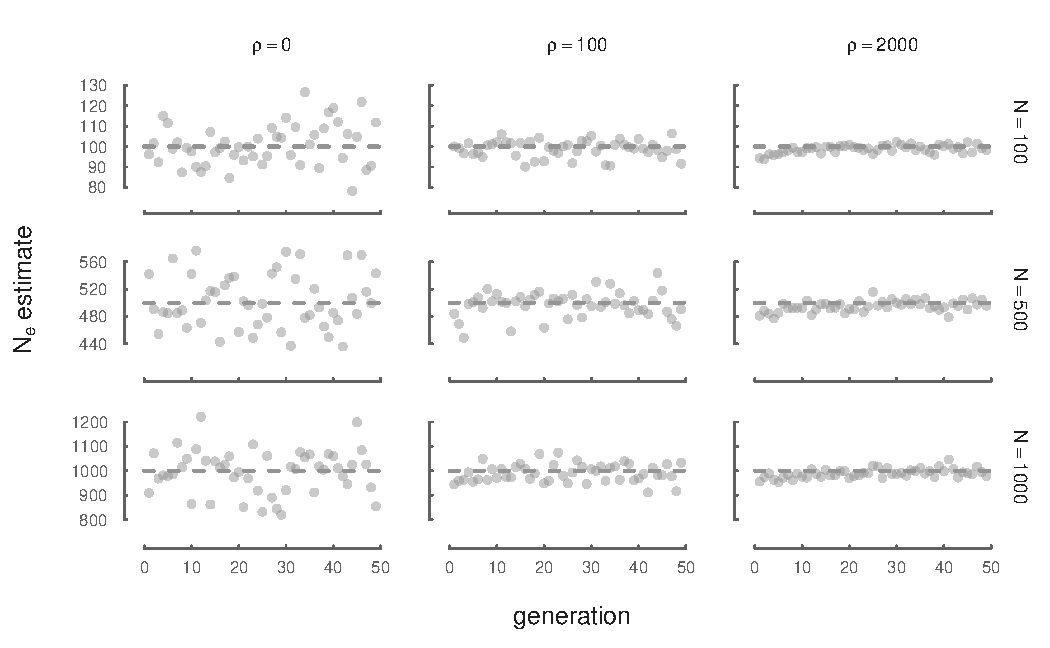
\includegraphics{./images/supp-Ne-est-neutral.pdf} 
  
  \caption{$N_e$ estimated through time from neutral forward simulations is
  consistent with true $N$ across a variety of recombination $\rho$ and $N$
parameters. Here, we estimate $N_e$ with $\widehat{N_e} = \nicefrac{p(1-p)}{2
\var(\Delta p)}$ from neutral allele frequency changes.}

  \label{fig:ne-neut}
\end{figure}

\clearpage
\newpage

\subsubsection{Dynamics of Variances}

\begin{figure}[!ht]
  \centering
  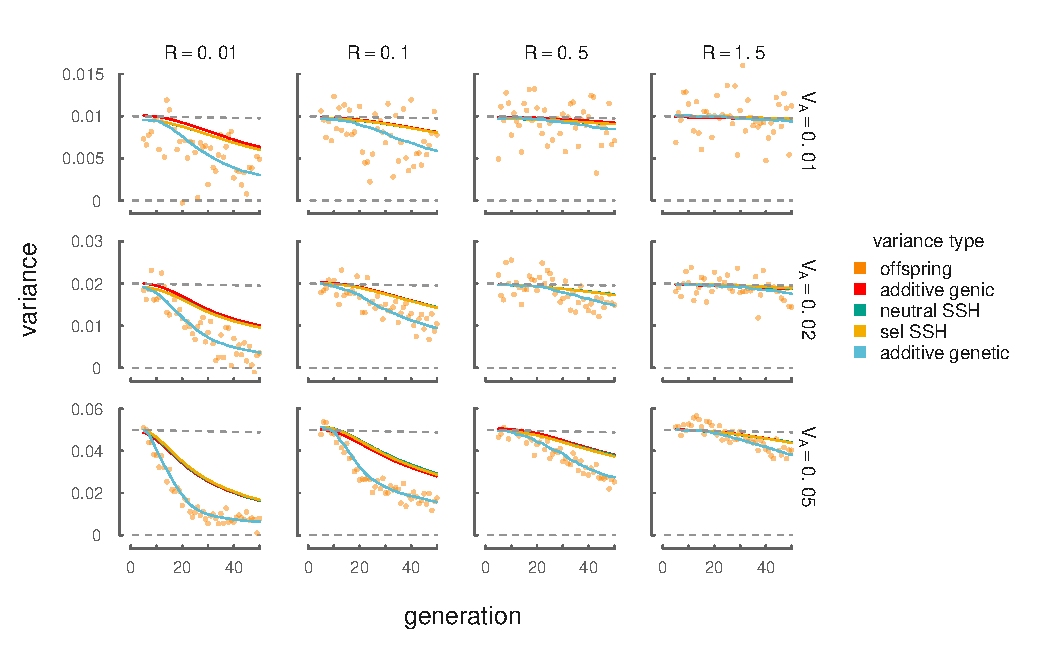
\includegraphics{./images/expfit-vark-types.pdf}
  \caption{The dynamics of different variances in our simulations, across a
    variety of initial target $V_A$ and $R$ levels. Orange points represent the
    empirical heritable variance in offspring (e.g. with the noise of the
    Wright--Fisher reproduction process removed). These closely track the
    additive genetic variance for the trait undergoing directional selection,
    $V_A = \var(z)$. The red line shows the dynamics of additive genic
    variance, $V_a = 2 \sum_l \alpha_l^2 p_l(1-p_l)$, which is closely tracked
  by both the selected (yellow line) and neutral (green line) sum of site
heterozygosity proxies described in Section \ref{sec:dyn-var}.}

  \label{fig:multilocus-expfit-vark}
\end{figure}

\clearpage
\newpage

\subsubsection{Supplementary Temporal Autocovariance Figures}

\begin{figure}[!ht]
  \centering
  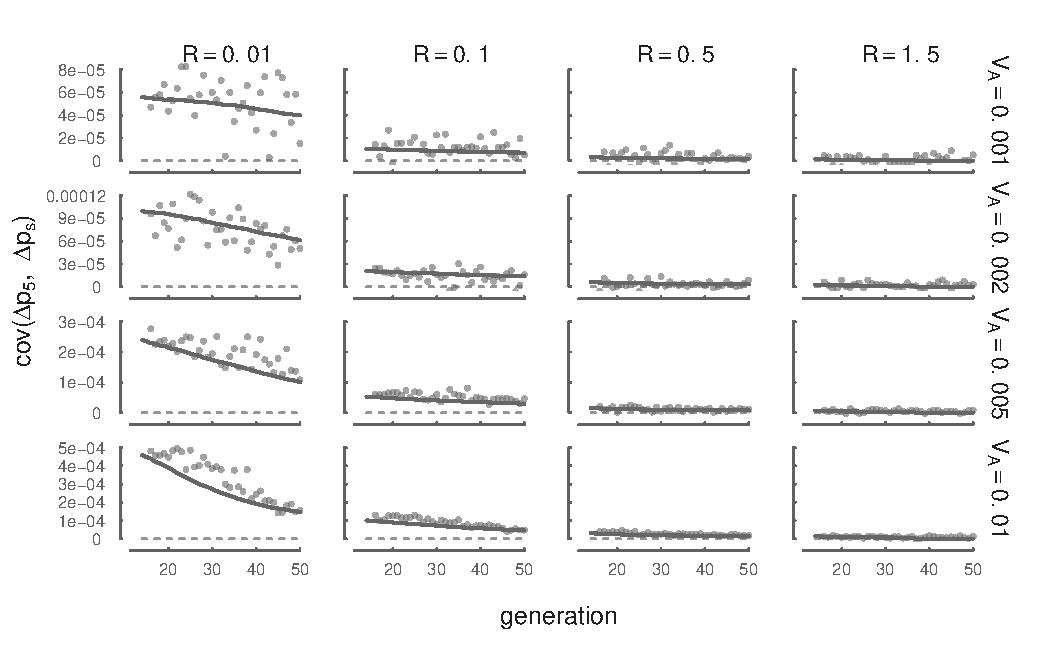
\includegraphics{./images/sim-pred13-covs-varyl.pdf}
  \caption{Each panel shows the temporal autocovariance $\cov(\Delta p_{13},
    \Delta p_s)$ on the y-axis, where $s$ varies along the x-axis. This is
    analogous to Figure \ref{fig:multilocus-expfit-sims} with a different
    reference generation ($t=13$), and compares the averaged simulation results
    (points) with the temporal autocovariance predicted by Equation
    \eqref{eq:multilocus-triangle} using the empirical additive genetic
    variance (curve). The covariances in these panels are weaker compared
    to those in Figure \ref{fig:multilocus-expfit-sims} because by generation
    13, additive genetic variance for fitness and the linkage disequilibria
    between neutral and selected sites has decayed.
}

\label{fig:multilocus-expfit-sims-gen13} 
\end{figure}


\begin{figure}[!ht]
  \centering
  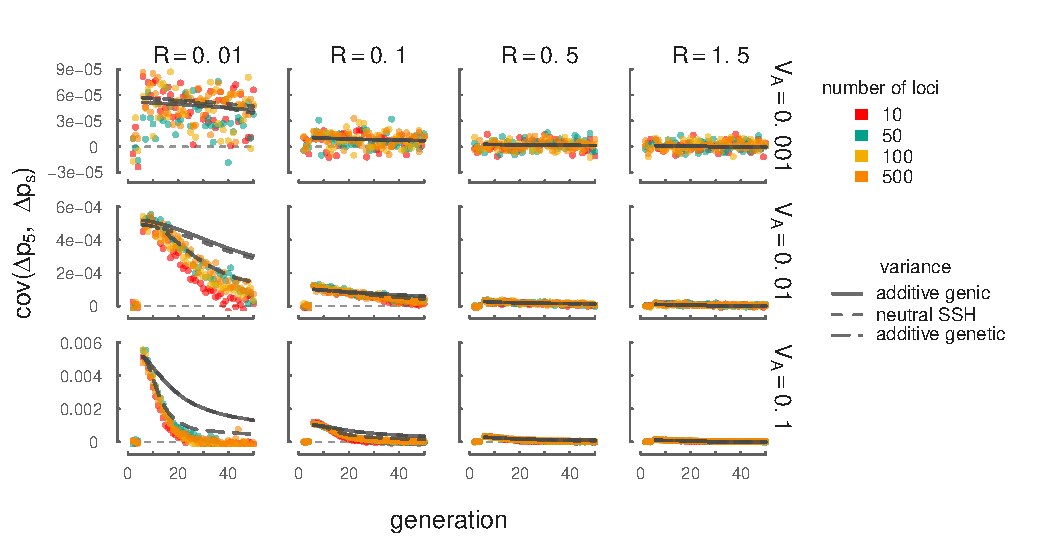
\includegraphics{./images/sim-pred-covs-varyl-va-oom.pdf}

  \caption{A version of Figure \ref{fig:multilocus-expfit-sims} with a subset
    of $V_A$ parameters used in our simulations that vary over orders of
    magnitude. This demonstrates that our theory using the empirical additive
    genic variance (solid gray line), additive genetic variance (long dashed
    gray line), and the neutral SSH proxy (short dashed gray lines) performs as
    described in Section \ref{sec:ml-sim-res} even when $V_A$ varies over
    orders of magnitude in a region. Higher variance in the empirical
    covariances with weak selection ($V_A = 0.001$) are due to chance covariances
    due to drift. The light gray dashed line depicts $\cov(\Delta p_5, \Delta p_s) =
  0$.}
  

  \label{fig:multilocus-expfit-sims-va-oom}
\end{figure}

\begin{figure}[!ht]
  \centering
  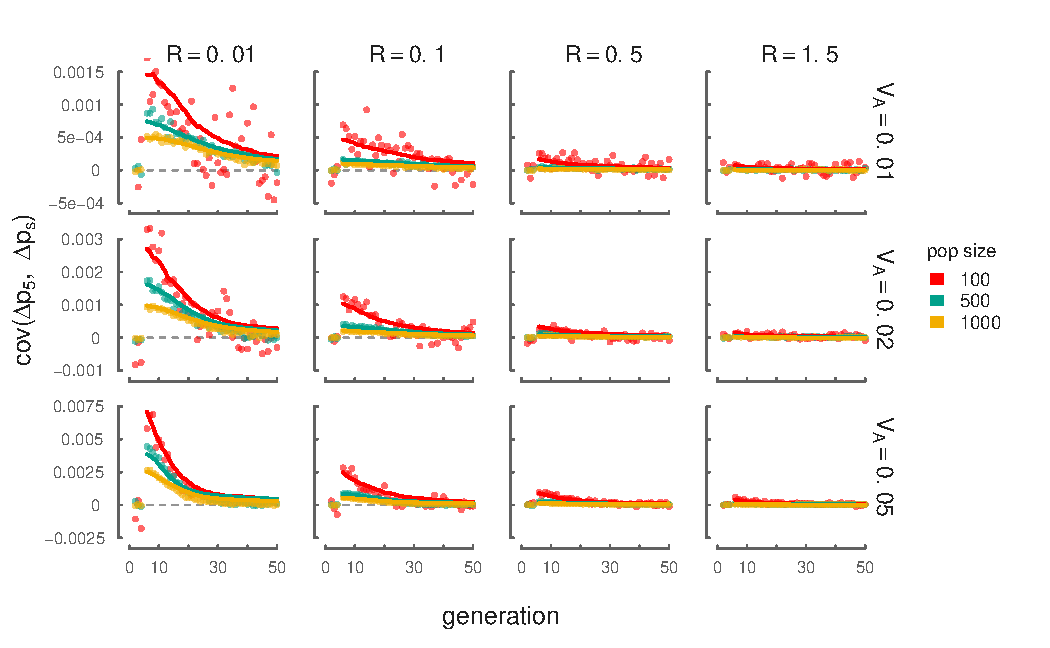
\includegraphics{./images/sim-pred-covs-varyn.pdf}

  \caption{A version of Figure \ref{fig:multilocus-expfit-sims} demonstrating
    temporal autocovariance simulation results and theoretical predictions with
    varying $N$. This demonstrates that our theory using the empirical additive
    genetic variance (lines) fits simulations across a variety of $N$
    parameters.  The light gray dashed line depicts $\cov(\Delta p_5, \Delta p_s) =
  0$. Note that the initial LD varies due to differing equilibrium levels of
LD from our burnin across varying $N$.}

  \label{fig:multilocus-expfit-sims-varyn}
\end{figure}


\end{document}
